\documentclass[conference]{IEEEtran}
\IEEEoverridecommandlockouts

\usepackage{cite}
\usepackage{algorithmic}
\usepackage{graphicx}
\usepackage{textcomp}
\usepackage{xcolor}
\usepackage{appendix}
\usepackage{booktabs}
\usepackage{amsmath}
\usepackage{amssymb}

\usepackage{url}

\usepackage[per-mode=symbol]{siunitx}
\usepackage[colorlinks=true, urlcolor=blue, linkcolor=black, citecolor=black]{hyperref}

\begin{document}

\title{Decentralized Spatial Negotiation via Utility-guided Residual Multi-agent Reinforcement Learning for Trajectory Generation}

%Residual Utility Learning: Residual Multi-Agent Policies over Behavioral Priors,

\author{\IEEEauthorblockN{Pedram Beigi}
\IEEEauthorblockA{\textit{The George Washington University}\\
Washington, DC, USA}
\and
\IEEEauthorblockN{Samer Hamdar}
\IEEEauthorblockA{\textit{The George Washington University}\\
Washington, DC, USA}
}

\maketitle

\begin{abstract}

Traffic in many developing regions operates under weak lane discipline, heterogeneous vehicle interactions, and decentralized negotiation of shared space. These environments challenge conventional lane-based trajectory prediction and motion planning frameworks, which typically rely on structured map priors and predefined leader--follower relationships. This paper presents a utility-guided residual multi-agent reinforcement learning framework for motion modeling in weakly structured non-lane-based traffic.

The proposed approach combines an interpretable utility-based behavioral model with a residual multi-agent reinforcement learning policy. The utility model encodes directional preference, speed incentive, collision risk, and proximity-aware interaction terms derived from behavioral and economic decision-making principles. Rather than learning motion policies from scratch, the reinforcement learning layer adaptively modulates the utility-driven behavior through residual policy learning, enabling context-dependent negotiation while every executed move remains a discrete utility maximizer under bicycle kinematics.

The framework is evaluated on a weak-lane multilane freeway corridor reconstructed from high-resolution aerial trajectories collected in Lebanon. The residual policy is benchmarked against classical continuous-space planners (ORCA, social force, DWA, MPPI), a Frenet-observation MAPPO baseline, and the calibrated utility prior under a shared closed-loop harness with vehicle-scale OBB lookahead inside the utility kernel. On the sparse freeway protocol, the prior and residual policy are collision-free, while MAPPO records $2.1$ contacts with the shortest travel time ($33.8\,\mathrm{s}$, arrival $0.93$) and pairwise planners record $0.3$--$3.2$. Residual MARL raises sparse arrival relative to the prior ($0.89$ versus $0.86$). Under denser spawn, residual collisions fall from $8.5$ to $7.1$ while MAPPO rises to $44.9$ despite $0.97$ arrival. Freezing kernel-scale residuals reverses the dense residual gain. Every residual move remains inside the same interpretable utility maximizer.

This work establishes a principled framework for integrating behavioral utility theory and multi-agent reinforcement learning for decentralized motion generation in weakly structured traffic environments. The code and pre-trained models are available at: \url{https://github.com/pebeigi/U-ResMARL}.

\end{abstract}

\begin{IEEEkeywords}
Motion Modeling, Reinforcement Learning, Multi-Agent Systems, Decision-Making Under Uncertainty, Trajectory Data, Model Calibration
\end{IEEEkeywords}

\section{Introduction}
\label{introduction}

In many developing countries, transportation systems operate under conditions that differ substantially from the structured, lane-disciplined traffic typically assumed in classical models \cite{chandra2004mixedtraffic, arasan2010heterogeneous, sleiman2026diffusion}. Weak rule enforcement, heterogeneous vehicle fleets, and informal negotiation of right-of-way produce complex interactions that challenge traditional traffic flow theory \cite{hoogendoorn2001state}. Such irregular behaviors including lateral encroachments, opportunistic yielding, and abrupt accelerations are prevalent in Lebanon, where infrastructure and enforcement limitations contribute to weak-lane and non-standard driving patterns \cite{xu2018nonlane}. Accurately representing these settings requires empirical data and modeling approaches that remain valid when lane structure and deterministic leader-follower assumptions are only weakly satisfied.

Recent advances in aerial data collection enable direct observation of naturalistic traffic with high spatial and temporal resolution. Drone-based video provides an unobstructed top-down view of vehicle motion, allowing large-scale extraction of trajectories while preserving behavioral authenticity \cite{zhou2017trajectorydrone}. This study focuses on an aerial trajectory dataset collected in Jounieh, Lebanon, over a multilane freeway segment characterized by non-lane-based longitudinal interactions and informal lateral negotiation. Roundabout geometries with opportunistic merging remain an important future evaluation setting, but all residual-learning and benchmarking experiments reported here are confined to the freeway corridor so that claims match the calibrated prior and closed-loop harness.

Microscopic vehicle models and modern trajectory forecasting frameworks remain central to representing vehicle interactions. However, state-of-the-art deep learning architectures (e.g., LaneGCN, VectorNet, Wayformer) predominantly assume strict lane centerlines, predefined map topologies, and structured drivable spaces. Consequently, they struggle to capture decentralized negotiation, emergent lane formation, and interaction-only forecasting without map priors in weak-lane environments. Furthermore, while Multi-Agent Reinforcement Learning (MARL) offers a pathway to game-theoretic trajectory generation, standard MARL formulations frequently fail in traffic applications. These failures stem from enormous action spaces, sparse rewards, collision instability, and a lack of human behavioral priors, ultimately yielding physically unrealistic driving behavior.

To bridge this gap, we introduce a utility-guided residual MARL architecture specifically designed for unstructured, non-lane-based traffic. By decoupling human behavioral priors from deep policy learning, the proposed framework avoids the pitfalls of blind reinforcement learning. The architecture operates through a four-stage process:

\begin{itemize}
    \item \textbf{Stage 1: Utility Prior:} An interpretable baseline utility formulation ($U_{base}$) captures directional preference, collision risk, and speed incentive. The additive structure is prospect-\emph{inspired} (asymmetric progress/risk trade-offs) rather than a Kahneman--Tversky value/weighting function.
    \item \textbf{Stage 2: Local Neighborhood Encoding:} Each agent observes a fixed budget of nearest neighbors (relative position and velocity) together with corridor clearances, yielding a fully decentralized observation.
    \item \textbf{Stage 3: RL Residual:} Instead of learning raw control actions, a shared residual policy learns a parameter adjustment $\Delta\Theta(o_{i})$ that modulates the underlying utility weights and collision-kernel scales.
    \item \textbf{Stage 4: Final Utility Maximization:} The executed action is obtained by discrete utility maximization under $\Theta_{i}=\mathrm{clip}(\Theta_{\mathrm{base}}+\Delta\Theta_{i})$, preserving physical realism, interpretability, and kinematic feasibility while enabling context-dependent negotiation.
\end{itemize}

Beyond reproducing vehicle kinematics, weak-lane and chaotic driving reflect asymmetric human decision-making under perceived risk. Prospect theory provides a principled framework to quantify such behaviors relative to reference points, highlighting how drivers trade off progress against conflict risk. The proposed residual MARL framework complements this by providing a data-driven mechanism to capture implicit interaction rules and spatial negotiation across multiple agents in dense settings.

The contributions of this study are:
\begin{itemize}
    \item Calibration of a twelve-parameter utility prior (including vehicle-scale collision-kernel widths) on Lebanon freeway aerial trajectories, with robust working parameters for downstream simulation.
    \item A utility-guided residual MARL policy that learns nine-dimensional parameter adjustments $\Delta\Theta$ (including $\Delta\sigma_{\parallel},\Delta\sigma_{\perp}$) rather than raw controls, preserving interpretability under bicycle kinematics.
    \item A matched-seed closed-loop benchmark on the freeway corridor comparing residual MARL to ORCA, social force, DWA, MPPI, MAPPO, and the frozen utility prior, with a kernel-scale ablation and a dense-negotiation stress protocol.
    \item Evidence that the lookahead-equipped prior is collision-free on the sparse protocol; residual MARL then improves sparse arrival and lowers mean dense collisions relative to the prior (only when $\Delta\sigma$ is enabled), whereas unconstrained MAPPO wins arrival by leaving the human speed band and colliding under crowding.
\end{itemize}

This integrated approach establishes a robust foundation for modeling heterogeneous, non-lane-based traffic using a principled combination of deterministic, stochastic, and learning-based methods.

\section{Literature Review}
\label{lit_review}

Modeling vehicle motion in traffic systems has been a central topic in transportation research, with a wide range of approaches developed to describe how drivers interact with their surroundings. Traditional models largely rely on structured, lane-based assumptions, while more recent work has explored interaction-driven, behavioral, and learning-based frameworks to better capture complex and unstructured traffic environments. This section reviews the relevant literature across four key domains: classical microscopic models, non-lane-based traffic modeling, interaction-based motion models, and data-driven learning approaches.

\subsection{Classical Microscopic Traffic Models}
Microscopic traffic flow models describe the behavior of individual vehicles, typically focusing on how drivers adjust acceleration in response to surrounding traffic conditions. Among the most widely used formulations are car-following models such as the Intelligent Driver Model (IDM) \cite{treiber2000congested, treiber2013traffic}, the Full Velocity Difference Model (FVDM) \cite{bando1995dynamical}, and Gipps’ model. These models assume a well-defined leader--follower relationship and describe vehicle acceleration as a function of spacing, relative speed, and desired velocity.

Such formulations have been successful in modeling traffic dynamics on structured highways with strong lane discipline. Their parameters are often interpretable, capturing driver preferences for desired speed, time headway, and acceleration behavior. However, their reliance on a single leading vehicle and strictly longitudinal interactions limits their applicability in environments where lane structure is weak or absent. In such cases, interactions become inherently two-dimensional, and drivers may respond simultaneously to multiple neighboring vehicles rather than a single leader.

\subsection{Non-Lane-Based and Heterogeneous Traffic}
In many developing regions, traffic is characterized by weak lane discipline, heterogeneous vehicle types, and informal negotiation of space. These conditions give rise to non-lane-based traffic, where vehicles do not adhere to fixed lanes and instead move in a continuous two-dimensional space. Several studies have highlighted the limitations of classical car-following models in such environments and proposed adaptations to account for lateral interactions and multiple leaders.

Research on heterogeneous traffic flow emphasizes the importance of capturing interactions beyond a single leader, including lateral encroachments and opportunistic maneuvers. Approaches often rely on data-driven definitions of interaction neighborhoods or extend classical models to consider multiple surrounding vehicles. Despite these efforts, many models retain a fundamentally longitudinal structure and struggle to fully represent the decentralized and multi-agent nature of non-lane-based traffic. This has motivated the exploration of alternative modeling paradigms that operate directly in continuous space.

\subsection{Interaction-Based and Continuous-Space Models}
To address the limitations of lane-based formulations, a class of models has emerged that represents vehicle motion through local interactions in continuous space. One prominent example is the Social Force Model (SFM) \cite{helbing1995socialforce}, originally developed for pedestrian dynamics. In this framework, agents are subject to attractive forces toward desired motion and repulsive forces from nearby agents, enabling flexible modeling of dense and unstructured interactions.

In robotics and multi-agent systems, collision avoidance has been extensively studied using velocity-based approaches such as Velocity Obstacles (VO) and Reciprocal Velocity Obstacles (RVO). Building on these concepts, the Optimal Reciprocal Collision Avoidance (ORCA) framework \cite{berg2008reciprocal, berg2011reciprocal} formulates collision avoidance as a set of linear constraints in velocity space. Each agent computes a feasible set of collision-free velocities by considering pairwise interactions with neighboring agents and selects the velocity closest to its preferred motion.

These approaches are well-suited for modeling multi-agent interactions in continuous space and can scale to dense environments without requiring explicit lane definitions. However, they are primarily geometric and deterministic in nature, focusing on collision avoidance rather than behavioral realism. As a result, they do not explicitly capture driver heterogeneity, risk perception, or decision-making under uncertainty, which are critical components of real-world driving behavior.

\subsection{Behavioral and Stochastic Models}
Human driving behavior is inherently stochastic and influenced by subjective perceptions of risk and reward. Behavioral models aim to capture these aspects by incorporating psychological and decision-theoretic principles into motion modeling. Prospect Theory \cite{kahneman1979prospect} provides a well-established framework for modeling decision-making under risk, where outcomes are evaluated relative to a reference point and losses are weighted more heavily than gains.

In transportation research, prospect-theoretic formulations have been applied to problems such as route choice and gap acceptance, demonstrating the importance of asymmetric risk perception in driving decisions. These models provide a natural way to represent aggressive or conservative behavior, particularly in environments where drivers must continuously evaluate trade-offs between progress and safety.

Despite their strengths, most behavioral models are not formulated in a fully continuous two-dimensional setting and often rely on simplified interaction assumptions. Integrating behavioral decision-making with realistic multi-agent interactions remains an open challenge, particularly in non-lane-based traffic environments.

\subsection{Learning-Based and Multi-Agent Approaches}
Recent advances in machine learning have led to the development of data-driven approaches for modeling vehicle behavior, particularly through reinforcement learning. In this paradigm, agents learn control policies by interacting with an environment and optimizing a reward function that encodes desired objectives such as safety, efficiency, and comfort.

Multi-Agent Reinforcement Learning (MARL) extends this framework to settings where multiple agents interact simultaneously. The Multi-Agent Deep Deterministic Policy Gradient (MADDPG) algorithm \cite{lowe2017multi} is a widely used approach for continuous control problems, enabling agents to learn decentralized policies while leveraging centralized training. Such methods have been applied to autonomous driving scenarios, demonstrating the ability to capture complex interaction patterns and emergent behaviors.

Learning-based approaches offer significant flexibility and can adapt to complex, high-dimensional environments without requiring explicit modeling assumptions. However, they often lack interpretability and depend heavily on the design of reward functions and training data. Moreover, their behavior may be difficult to analyze or generalize beyond the training conditions.

\subsection{Research Gap and Contribution}
The existing literature provides a diverse set of tools for modeling traffic dynamics, ranging from deterministic interaction-based models to stochastic behavioral formulations and data-driven learning approaches. However, these paradigms are typically studied in isolation, and direct comparisons across fundamentally different modeling assumptions remain limited.

In particular, there is a lack of unified frameworks that evaluate deterministic collision-avoidance models, stochastic decision-theoretic models, and multi-agent learning approaches within the same non-lane-based traffic context. This gap is especially relevant for heterogeneous traffic environments, where interactions are multi-dimensional and behavior is highly variable.

To address this limitation, the present study develops a comparative freeway evaluation that places a calibrated utility prior and a residual MARL adapter alongside classical continuous-space planners (ORCA, social force, DWA, MPPI) and unconstrained MAPPO in a shared closed-loop harness. The comparison is designed so that residual MARL is judged as a calibrated, interpretable generator---not as a substitute for pairwise geometric avoidance or a speed-maximizing RL policy.

\subsection{Trajectory Data}
The rapid growth of aerial data collection has transformed how chaotic and non-lane-based traffic patterns are observed and modeled. Unmanned aerial vehicles (UAVs) provide a top-down view that can simultaneously capture trajectories of all road users, including vehicles, cyclists, and pedestrians, over complex geometries. A UAV-based methodological framework was developed for multivehicle trajectory extraction at urban roundabouts, demonstrating that drones can capture detailed kinematic profiles and gap-acceptance behavior that are difficult to observe using fixed cameras \cite{khan2018uav}. Other researchers used drones to analyze traffic flow at urban roundabouts, showing how high-resolution aerial imagery can reveal subtle lane encroachments, yielding patterns, and circulation strategies that are often invisible in aggregated loop-detector data \cite{brahimi2020drones}.

In parallel, several open datasets have emerged that provide high-fidelity trajectories from aerial views for intersections and roundabouts. Researchers introduced the TUMDOT-MUC dataset, a large-scale collection of multimodal trajectories (motorized vehicles and vulnerable road users) gathered by drone over multiple urban sites, specifically designed to support model calibration and safety analysis in complex multimodal environments \cite{kutsch2024tumdot}. Other researchers published a dataset of UAV-based aerial images with detailed vehicle annotations, enabling researchers to build and validate computer-vision pipelines for vehicle detection and, by extension, trajectory extraction in circular intersections \cite{puertas2022roundabout}. More recently, the MiTra dataset was released, which provides drone-based trajectories for freeways with ramps across all traffic states, illustrating how persistent aerial observation can be used to study microscopic behavior from free flow to congestion \cite{chaudhari2025mitra}.

Aerial data has also been leveraged for proactive safety analysis. The Extra Brake Required to Avoid a Crash (EBRAC) surrogate measure was proposed using drone-based image-recording data, quantifying near-crash conflicts at intersections by reconstructing detailed braking profiles and interaction dynamics \cite{huang2024ebrac}. This work illustrates how high-resolution trajectories can be transformed into interpretable safety indicators that directly reflect road-user maneuvers. Similar methodologies have been applied to other drone-based datasets to derive conflict-based safety metrics and evaluate how geometric design and control strategies affect risk.

\subsection{Research Gap}
Overall, the literature shows (i) strong evidence that weak lane discipline and heterogeneous traffic produce irregular, continuous-space interactions; (ii) a split between geometric collision-avoidance planners, behavioral utility models, and unconstrained MARL; and (iii) high-resolution aerial trajectories that make those methods testable on the same naturalistic scenes. What is still missing is a single generator that is \emph{at once} (a)~calibrated to observed choice, (b)~kinematically constrained and interpretable, and (c)~able to adapt that prior when crowding increases---without collapsing into either a pure collision-avoidance oracle or a reward-hacking speed policy.

This paper closes that gap on a Lebanon freeway corridor by calibrating a twelve-parameter utility prior, training a residual MARL adapter over that prior, and comparing the resulting policy in a shared harness to ORCA, social force, DWA, MPPI, MAPPO, and the frozen prior. Residual MARL occupies the intended intersection of those requirements; the two urban datasets in Appendix~\ref{app:datasets} probe whether the prior itself transfers when corridor geometry is replaced by destination-plus-curb encoding, without repeating the residual-learning study.

\section{METHODOLOGY}
This work proposes a utility-guided residual multi-agent reinforcement learning framework for motion generation in weakly structured non-lane-based traffic. Unlike conventional lane-based trajectory prediction approaches that rely on explicit lane markings, discrete lane topology, or predefined leader-follower relationships, the proposed framework models vehicle interactions directly in continuous two-dimensional space through decentralized utility maximization and adaptive behavioral learning.

Although lane markings are not imposed as discrete behavioral modes, agents remain constrained by the physical geometry of the drivable corridor. Corridor-aligned Frenet features and boundary penalties are therefore used to encode physical road geometry without reducing behavior to classical lane keeping.

The proposed framework combines two complementary components:
\begin{enumerate}
    \item an interpretable utility-based behavioral prior that captures directional preference, collision risk, speed regulation, proximity/progress incentive, and corridor adherence;
    \item a residual multi-agent reinforcement learning policy that adaptively modulates selected utility parameters according to the surrounding traffic context.
\end{enumerate}

Rather than directly learning low-level control actions or trajectories from scratch, the reinforcement learning layer learns residual behavioral adaptations over a structured utility formulation. This preserves physical interpretability and kinematic feasibility while enabling emergent negotiation behaviors in dense heterogeneous traffic.

\subsection{Problem Formulation}
Traffic is modeled as a decentralized multi-agent system operating in continuous two-dimensional space. Let $\mathcal{A}=\{1,2,\ldots,N\}$ denote the set of traffic agents. Each agent $i\in\mathcal{A}$ is represented by a continuous kinematic state
\begin{equation}
s_{i}^{t}=\big[x_{i}^{t},y_{i}^{t},v_{i}^{t},\theta_{i}^{t}\big],
\end{equation}
where $(x_{i}^{t},y_{i}^{t})$ denotes spatial position, $v_{i}^{t}\ge 0$ denotes speed magnitude, and $\theta_{i}^{t}$ denotes heading angle.

Each agent observes a local neighborhood of at most $K$ nearest neighbors within a perception radius $R_{p}$:
\begin{equation}
\mathcal{N}_{i}^{t}
=
\Big\{
j\in\mathcal{A}\setminus\{i\}
\;\Big|\;
\|r_{j}^{t}-r_{i}^{t}\|_{2}\le R_{p}
\Big\}_{1:K},
\end{equation}
where $r_{i}^{t}=(x_{i}^{t},y_{i}^{t})$ and the subset retains the $K$ closest neighbors by Euclidean distance.

The objective of each agent is to generate feasible motion that progresses along the corridor, avoids collisions, remains within drivable boundaries, and negotiates shared space with neighboring agents. Unlike classical lane-based formulations, agents are not restricted to discrete lane IDs or fixed leader-follower roles.

\subsection{Utility-Based Behavioral Prior}
The nominal motion behavior of each agent is governed by a utility-maximization process over a discrete control-candidate set. At each time step, agent $i$ evaluates candidates generated from a finite grid of longitudinal acceleration and steering values,
\begin{equation}
\mathcal{G}
=
\big\{(a,\delta)\big\}
=
\mathcal{A}_{\text{acc}}\times\mathcal{A}_{\text{steer}},
\end{equation}
and selects the candidate that maximizes expected utility after one-step kinematic bicycle rollout:
\begin{equation}
(a_{i}^{*},\delta_{i}^{*})
=
\arg\max_{(a,\delta)\in\mathcal{G}}
U_{i}\!\left(s_{i}'(a,\delta);\Theta_{i}\right),
\end{equation}
where $s_{i}'(a,\delta)$ is the predicted next state obtained from the bicycle dynamics and $\Theta_{i}$ denotes the agent's behavioral utility parameters.

The total utility consists of five components:
\begin{equation}
U_{i}
=
U_{\mathrm{dir}}
+
U_{\mathrm{speed}}
+
U_{\mathrm{dist}}
-
U_{\mathrm{col}}
-
U_{\mathrm{path}}.
\label{eq:utility}
\end{equation}

\subsubsection{Directional Utility}
Directional utility encourages motion aligned with the local corridor tangent rather than an unconstrained destination vector. Let
\begin{equation}
\hat{m}_{i}
=
\frac{r_{i}'-r_{i}}{\|r_{i}'-r_{i}\|_{2}}
\end{equation}
denote the unit move direction induced by a candidate next position $r_{i}'$, and let $\hat{t}_{i}$ denote the unit tangent of the corridor centerline at the ego agent's current projection. Then
\begin{equation}
U_{\mathrm{dir}}
=
S_{\theta}\,
\hat{m}_{i}^{\top}\hat{t}_{i},
\end{equation}
where $S_{\theta}>0$ controls directional sensitivity. This formulation remains valid for both positive- and negative-direction traffic because directionality is defined by the corridor orientation rather than the global $x$-axis.

\subsubsection{Speed Incentive}
Speed incentive rewards candidate rollout speeds that are close to a desired speed $v_{\mathrm{des},i}$. Because scalar speed is non-negative, reverse motion is represented through heading rather than negative speed. For a candidate speed $v_{i}'$, define the symmetric closeness ratio
\begin{equation}
\rho_{i}
=
\frac{\min(v_{i}',v_{\mathrm{des},i})}{\max(v_{i}',v_{\mathrm{des},i})}\in(0,1].
\end{equation}
The speed utility is then
\begin{equation}
U_{\mathrm{speed}}
=
S_{v}\,
\frac{\rho_{i}}{1+\rho_{i}^{(\xi_{i}-1)/2}},
\end{equation}
where $S_{v}>0$ scales the term and $\xi_{i}>1$ controls how sharply the reward decreases under speed mismatch. The maximum occurs at $v_{i}'=v_{\mathrm{des},i}$, and overspeeding and underspeeding are penalized symmetrically.

\subsubsection{Proximity Incentive}
Proximity utility encourages progress toward a local reference point expressed in corridor Frenet coordinates. Let $(s_{i}',n_{i}')$ be the longitudinal and lateral projections of the candidate next position onto the corridor, and let $(s_{\mathrm{ref}},n_{\mathrm{ref}})$ be the corresponding projection of a local reference location (e.g., a short-horizon target state). The anisotropic effective distance is
\begin{equation}
d_{\mathrm{eff}}
=
w_{x}|s_{i}'-s_{\mathrm{ref}}|
+
w_{y}|n_{i}'-n_{\mathrm{ref}}|.
\end{equation}
A speed-dependent perception horizon,
\begin{equation}
H_{p}
=
\max\!\left(\kappa v_{i},\, H_{\min}\right),
\end{equation}
normalizes this distance, yielding
\begin{equation}
U_{\mathrm{dist}}
=
\frac{S_{d}}{1+(d_{\mathrm{eff}}/H_{p})^{\gamma}},
\end{equation}
where $S_{d}>0$ caps the reward magnitude and $\gamma>0$ controls how quickly the incentive decays for distant candidates.
%% new collision part
\subsubsection{Collision-Risk Utility}
In weakly structured environments, collision risk cannot be reduced to hard geometric overlaps alone. Instead, collision risk is modeled by comparing the candidate next pose of the ego agent with short-horizon predictions of neighbors, expressed in the ego body frame and measured relative to vehicle footprints (length $L$, width $W$; defaults $4.5\,\mathrm{m}\times 1.8\,\mathrm{m}$).

For neighbor $j$, the predicted future position after the candidate arrival time $\Delta t$ is obtained by constant-velocity extrapolation,
\begin{equation}
\mu_{j}
=
r_{j}+v_{j}\Delta t.
\end{equation}
Let $\Delta r_{i'j}=R(\psi_{i'})^{\top}(r_{i}'-\mu_{j})$ be this relative vector in the candidate heading frame ($+x$ forward). Surface gaps beyond the same-size footprints are
\begin{equation}
g_{\parallel}=\max\!\bigl(0,\,|\Delta r_{i'j}^{(x)}|-L\bigr),\qquad
g_{\perp}=\max\!\bigl(0,\,|\Delta r_{i'j}^{(y)}|-W\bigr),
\end{equation}
so overlapping oriented boxes yield zero gap. Soft presence uses an anisotropic Gaussian on these gaps,
\begin{equation}
P_{j,i'}
=
\exp\!\left(
-\frac{1}{2}
\left[
\left(\frac{g_{\parallel}}{\sigma_{\parallel}}\right)^{2}
+
\left(\frac{g_{\perp}}{\sigma_{\perp}}\right)^{2}
\right]
\right),
\end{equation}
with calibrated (and residual-adapted) scales $\sigma_{\parallel},\sigma_{\perp}$. Aggregating over neighbors and capping cumulative risk yields
\begin{equation}
U_{\mathrm{col}}
=
w_{c}\,
\min\!\left(
\sum_{j\in\mathcal{N}_{i}}
P_{j,i'}
,\,1
\right),
\end{equation}
where $w_{c}>0$ controls collision aversion. Candidate selection additionally rejects bicycle rollouts whose predicted OBB overlaps a neighbor when a collision-free alternative exists, and speed alignment uses the nearest ahead neighbor as a car-following reference when one is present.

Calibration scores this kernel at the data/control interval $\Delta t$ (one predicted neighbor pose). Closed-loop residual training and benchmarking additionally query the same OBB kernel along a short constant-velocity horizon ($1.5\,\mathrm{s}$, four substeps). Geometric planners in the benchmark do \emph{not} use that lookahead at decision time; they are scored with the same OBB contact detector after each executed step.

\subsubsection{Path Adherence and Boundary Constraints}
Although agents negotiate laterally inside the corridor without discrete lane constraints, they remain subject to infrastructural boundaries. A path-adherence penalty discourages proximity to corridor edges and off-road intrusion:
\begin{equation}
U_{\mathrm{path}}
=
w_{\ell}\big(1-e^{-\beta\,\ell_{i}^{2}}\big),
\end{equation}
where $\ell_{i}$ is a non-negative lateral clearance residual relative to the corridor boundary (including an optional near-edge buffer), $w_{\ell}$ scales the penalty magnitude, and $\beta$ controls the sharpness of the transition near the boundary.

\subsection{Kinematic Bicycle Candidate Generation}
Each control candidate $(a,\delta)$ is rolled out through a one-step kinematic bicycle model. Given the current ego state $(x,y,v,\theta)$ and wheelbase $L$,
\begin{equation}
\begin{aligned}
v'
&=
\mathrm{clip}\!\left(v+a\Delta t,\,0,\,v_{\max}\right),\\
\theta'
&=
\theta+\frac{v}{L}\tan\delta\,\Delta t,\\
x'
&=
x+v'\cos\theta'\,\Delta t,\\
y'
&=
y+v'\sin\theta'\,\Delta t.
\end{aligned}
\end{equation}
Thus the utility evaluation is performed over the resulting candidate next state $(x',y',v',\theta')$, rather than over free speed/heading pairs. Importantly, $v'$ is constrained to be non-negative; negative-direction travel is represented by heading aligned with the corridor orientation.

\subsection{Residual Multi-Agent Reinforcement Learning}
Fixed utility parameters cannot fully capture adaptive negotiation, contextual yielding, temporary aggressiveness, or emergent interaction strategies. Therefore, a residual multi-agent reinforcement learning (MARL) policy modulates a subset of the utility parameters according to the local observation.

The residual policy is
\begin{equation}
\Delta\Theta_{i}^{t}=\pi_{\phi}(o_{i}^{t}),
\end{equation}
and the adapted parameters are
\begin{equation}
\Theta_{i}^{t}
=
\mathrm{clip}\!\left(
\Theta_{i}^{\mathrm{base}}+\Delta\Theta_{i}^{t}
\right).
\end{equation}
Motion is then selected by utility maximization under the adapted parameters:
\begin{equation}
(a_{i}^{*},\delta_{i}^{*})
=
\arg\max_{(a,\delta)\in\mathcal{G}}
U_{i}\!\left(s_{i}'(a,\delta);\Theta_{i}^{t}\right).
\end{equation}
Thus the RL policy does not directly output accelerations or trajectories; it only modulates the interpretable behavioral prior.

\subsection{Policy Observation Space}
Each agent receives a fully decentralized local observation in corridor Frenet coordinates for the ego vehicle and in the ego body frame for neighbors (world $(x,y)$ on this diagonal corridor saturates a fixed Cartesian scale):
\begin{equation}
\begin{aligned}
o_{i}^{t}
=
\Big[
&s_{i},\;n_{i},\;v_{i},\;\tilde\theta_{i},\;\tilde\theta_{\mathrm{goal},i},\\
&d_{\mathrm{lower},i},\;d_{\mathrm{upper},i},\\
&\big\{\Delta x^{\mathrm{body}}_{ij},\,\Delta y^{\mathrm{body}}_{ij},\,\Delta v_{x,ij}^{\mathrm{body}},\,\Delta v_{y,ij}^{\mathrm{body}}\big\}_{j\in\mathcal{N}_{i}}
\Big],
\end{aligned}
\end{equation}
where $(s_{i},n_{i})$ are the longitudinal/lateral projections onto the PCA tube, $\tilde\theta_{i}$ and $\tilde\theta_{\mathrm{goal},i}$ are heading errors relative to the local tangent, $d_{\mathrm{lower},i}$ and $d_{\mathrm{upper},i}$ are clearances to the corridor bounds, and missing neighbors are zero-padded up to the fixed neighbor budget $K$.

\subsection{Residual Action Space}
The policy adapts both the magnitude and sensitivity of selected utility components, including the collision-kernel scales. The continuous residual action is nine-dimensional:
\begin{equation}
\Delta\Theta_{i}^{t}
=
\big[
\Delta S_{v},\;
\Delta S_{\theta},\;
\Delta S_{d},\;
\Delta w_{c},\;
\Delta \xi_{i},\;
\Delta \gamma,\;
\Delta w_{\ell},\;
\Delta \sigma_{\parallel},\;
\Delta \sigma_{\perp}
\big].
\end{equation}
The remaining utility parameters $(w_{x},w_{y},\beta)$ are treated as fixed geometric/shape priors in the current implementation. Residual actions are bounded (tanh-scaled per coordinate) and clipped to keep $\Theta_{i}^{t}$ within physically valid ranges.

\subsection{Reward Function}
The residual policy is trained with a multi-objective reward balancing progress, safety, control smoothness, and boundary feasibility:
\begin{equation}
R_{i}=w_{1}R_{\mathrm{progress}}+w_{2}R_{\mathrm{safety}}+w_{3}R_{\mathrm{smooth}}+R_{\mathrm{boundary}}
\end{equation}

The individual terms are
\begin{equation}
\label{eq:R_progress}
R_{\mathrm{progress}}
= v_{i}\cos(\theta_{i}-\theta_{\mathrm{tan},i}),
\end{equation}
where $\theta_{\mathrm{tan},i}$ is the local corridor tangent angle.
Let $g_{ij}=\|r_{j}-r_{i}\|_{2}-L$ be the centre-to-centre gap minus vehicle length. Contact-aware safety is
\begin{equation}
\label{eq:R_safety}
R_{\mathrm{safety}}
=
\sum_{j\in\mathcal{N}_{i}}
\begin{cases}
-16\,(1-g_{ij}), & g_{ij}\le 0,\\
-\exp(-g_{ij}/2), & g_{ij}>0.
\end{cases}
\end{equation}
An additional penalty of $8$ is subtracted from each agent involved in an OBB contact at that step. Smoothness is
\begin{equation}
\label{eq:R_smooth}
R_{\mathrm{smooth}}
= -\left(a_{i}^{2}+\lambda_{\delta}\delta_{i}^{2}\right).
\end{equation}

\begin{equation}
\label{eq:R_boundary}
R_{\mathrm{boundary}}
=
\begin{cases}
\begin{aligned}
-&\bigl(C_{\mathrm{out}}
+c_{\mathrm{depth}}\min(d_{\mathrm{out}},d_{\max})\bigr),
\\[-2pt]
&\hspace{1.5em}\text{outside corridor},
\end{aligned}
\\[4pt]
0, \quad \text{otherwise}.
\end{cases}
\end{equation}

where $a_{i}$ and $\delta_{i}$ are the executed bicycle controls, $\lambda_{\delta}$ weights steering cost, $C_{\mathrm{out}}>0$ is a base off-corridor penalty that exceeds the largest per-step progress reward, $d_{\mathrm{out}}$ is the penetration depth beyond the corridor edge, and $c_{\mathrm{depth}}$ provides a capped inward gradient ($d_{\max}$ prevents return-scale blow-up for untrained policies). An optional trajectory-matching term may be included when ground-truth imitation targets are available; in the present experiments it is set to zero.

\subsection{Training Procedure}
The residual policy is trained under centralized training and decentralized execution (CTDE). Episodes are initialized from observed traffic states derived from drone-based trajectory data. At each step:
\begin{enumerate}
    \item each agent receives its local observation $o_{i}^{t}$;
    \item the policy outputs residuals $\Delta\Theta_{i}^{t}$;
    \item utility parameters are updated and clipped;
    \item discrete acceleration/steering candidates are generated and scored by the modulated utility;
    \item the maximum-utility bicycle transition is executed.
\end{enumerate}
Importantly, the learned policy never directly commands unconstrained trajectories. Vehicle motion remains governed by utility maximization and kinematic bicycle constraints, preserving interpretability while enabling complex emergent interactions in weakly structured traffic.

\section{Data Collection and Trajectory Extraction}
\label{data_extraction}

This study uses high-resolution aerial vehicle trajectories collected over multilane freeway segments in Jounieh, Lebanon, under weak lane discipline and heterogeneous traffic conditions. Traffic was recorded with a drone in a near-stationary hover, providing a top-down view that reduces occlusions and supports simultaneous tracking of interacting vehicles. The site exhibits pronounced non-lane-based longitudinal and lateral interactions, including informal gap negotiation and shockwave-like disturbance propagation.

Trajectory extraction and site characterization are documented in detail by Khoueiry et al. \cite{khoueiry2025universal}, readers are referred to \cite{khoueiry2025universal} for the full data-collection protocol and extraction pipeline. In this paper, we restrict attention to passenger-vehicle trajectories with valid kinematic transitions and use corridor-aligned geometry derived from the observed streams as the spatial reference for utility evaluation. Two additional environments---a compact roundabout in Jounieh and the TGSIM Foggy Bottom street network---are used only for environment-based utility calibration and are documented in Appendix~\ref{app:datasets}.

\section{Calibration Methodology}
\label{sec:calibration_methodology}

The utility model in Eq.~\eqref{eq:utility} (directional alignment, speed alignment, proximity reward, collision penalty, and boundary adherence) contains twelve free parameters
\[
\theta=\bigl(S_\theta,\,S_v,\,\xi_i,\,S_d,\,\gamma,\,w_x,\,w_y,\,w_c,\,w_\ell,\,\beta,\,\sigma_{\parallel},\,\sigma_{\perp}\bigr),
\]
including the collision-kernel scales. These parameters are calibrated from the Lebanon naturalistic trajectory set so that the discrete utility prior reproduces observed short-horizon motion before any residual policy is trained.

\paragraph{Data and candidate actions.}
Valid passenger-vehicle transitions with time step $\Delta t\in[0.05,0.2]$\,s yield $190{,}767$ usable state records. From this pool we draw $N_{\mathrm{s}}=2000$ one-step choice samples. At each sample, the ego agent is reconstructed in the corridor frame with neighboring vehicles inside a $60$\,m radius (at most six neighbors). Candidate controls are generated on the same acceleration--steering grid used in simulation
(acceleration $\in\{-3,\ldots,3\}$\,m/s$^2$, steering $\in[-0.45,0.45]$\,rad), producing a discrete action set $\mathcal{A}$. The observed next state is matched to the nearest candidate (target index) for likelihood evaluation.

\paragraph{Closed-loop windows.}
Because one-step ranking alone under-constrains $\theta$, we split vehicles into train/validation/test ($221$/$74$/$73$) and sample short trajectory windows of horizon $H=8$ steps ($300$/$100$/$100$). From the observed initial state of each window, the utility model repeatedly selects $\arg\max_{a\in\mathcal{A}} U(a;\theta)$ and the simulated pose/speed/heading are compared with the recorded trajectory. Working parameters are chosen on validation windows; test windows are held out.

\paragraph{Objective.}
Calibration minimizes a weighted composite loss
\begin{equation}
\begin{aligned}
J(\theta)
&=
\lambda_{\mathrm{cl}}\,L_{\mathrm{cl}}(\theta)
+
\lambda_{\mathrm{trk}}\,\frac{\bar r(\theta)}{r_0}
+
\lambda_{\mathrm{nll}}\,L_{\mathrm{nll}}(\theta),
\end{aligned}
\label{eq:calibration_objective}
\end{equation}
where $L_{\mathrm{cl}}$ is the mean closed-loop tracking error (position, with speed and heading penalties), $\bar r$ is the mean rank of the observed-like candidate among $\mathcal{A}$, $r_0=63$ normalizes rank, and $L_{\mathrm{nll}}$ is the mean softmax negative log-likelihood of the target candidate at temperature $T=0.25$. We use $\lambda_{\mathrm{cl}}=1$, $\lambda_{\mathrm{trk}}=1$, and $\lambda_{\mathrm{nll}}=0.1$, so closed-loop fidelity is the primary target and the one-step likelihood acts as a light regularizer.

\paragraph{Search and robust aggregation.}
Because $J(\theta)$ is non-convex and partially flat, we do not trust a single optimizer trajectory. Parameters are drawn uniformly in the search box of Table~\ref{tab:utility_search_bounds}. For each of $R=3$ independent restarts (different random seeds), $N_{\mathrm{t}}=400$ vectors are screened by the cheap one-step terms; the best $80$ candidates per restart ($240$ scored trials in total) are then evaluated with the closed-loop windows. Let $\theta^\star$ be the minimizer of $J$ and define the near-optimal cloud as all scored trials with
\[
J(\theta)\le J(\theta^\star)+\max\bigl(0.05,\,0.05\,|J(\theta^\star)|\bigr).
\]
If fewer than three trials satisfy this cutoff, the top ten scored trials are used instead. The \emph{robust} working point $\theta_{\mathrm{rob}}$ is the coordinate-wise median of that cloud. This aggregation reduces sensitivity to isolated lucky minima while retaining the same predictive performance up to a small objective gap. Quantiles of the top/near-optimal clouds supply recommended ranges for later sensitivity analysis; the Sobol study in the appendix predates this box and is labeled as such.

\begin{table}[t]
\centering
\caption{Search bounds used in utility calibration.}
\label{tab:utility_search_bounds}
\begin{tabular}{lcc}
\toprule
Parameter & Low & High \\
\midrule
$S_\theta$, $S_v$, $S_d$ & $0.05$ & $10$ \\
$\xi_i$ & $1.1$ & $10$ \\
$\gamma$, $\beta$ & $0.1$ / $0.01$ & $10$ \\
$w_x$, $w_y$ & $0.1$ & $10$ \\
$w_c$, $w_\ell$ & $0.01$ / $0.1$ & $1000$ \\
$\sigma_{\parallel}$ (m) & $0.5$ & $5$ \\
$\sigma_{\perp}$ (m) & $0.3$ & $2.5$ \\
\bottomrule
\end{tabular}
\end{table}


\section{Calibration Results}
\label{sec:calibration_results}

\paragraph{Fit quality.}
Across the $2000$ choice samples, the selected utility prior places the observed-like candidate at mean rank $5.72$ (robust working point $6.61$). The train-set minimizer attains $J(\theta^\star)=1.317$ (closed-loop loss $0.614$), while the robust median $\theta_{\mathrm{rob}}$---selected on held-out validation windows---yields $J=1.184$ (closed-loop loss $0.555$ on train windows, $0.576$ on validation) and a test closed-loop loss of $0.565$. Rank CDFs, margin histograms, and closed-loop loss distributions are summarized in Fig.~\ref{fig:calibration_fit_quality}.

\begin{figure*}[!t]
\centering
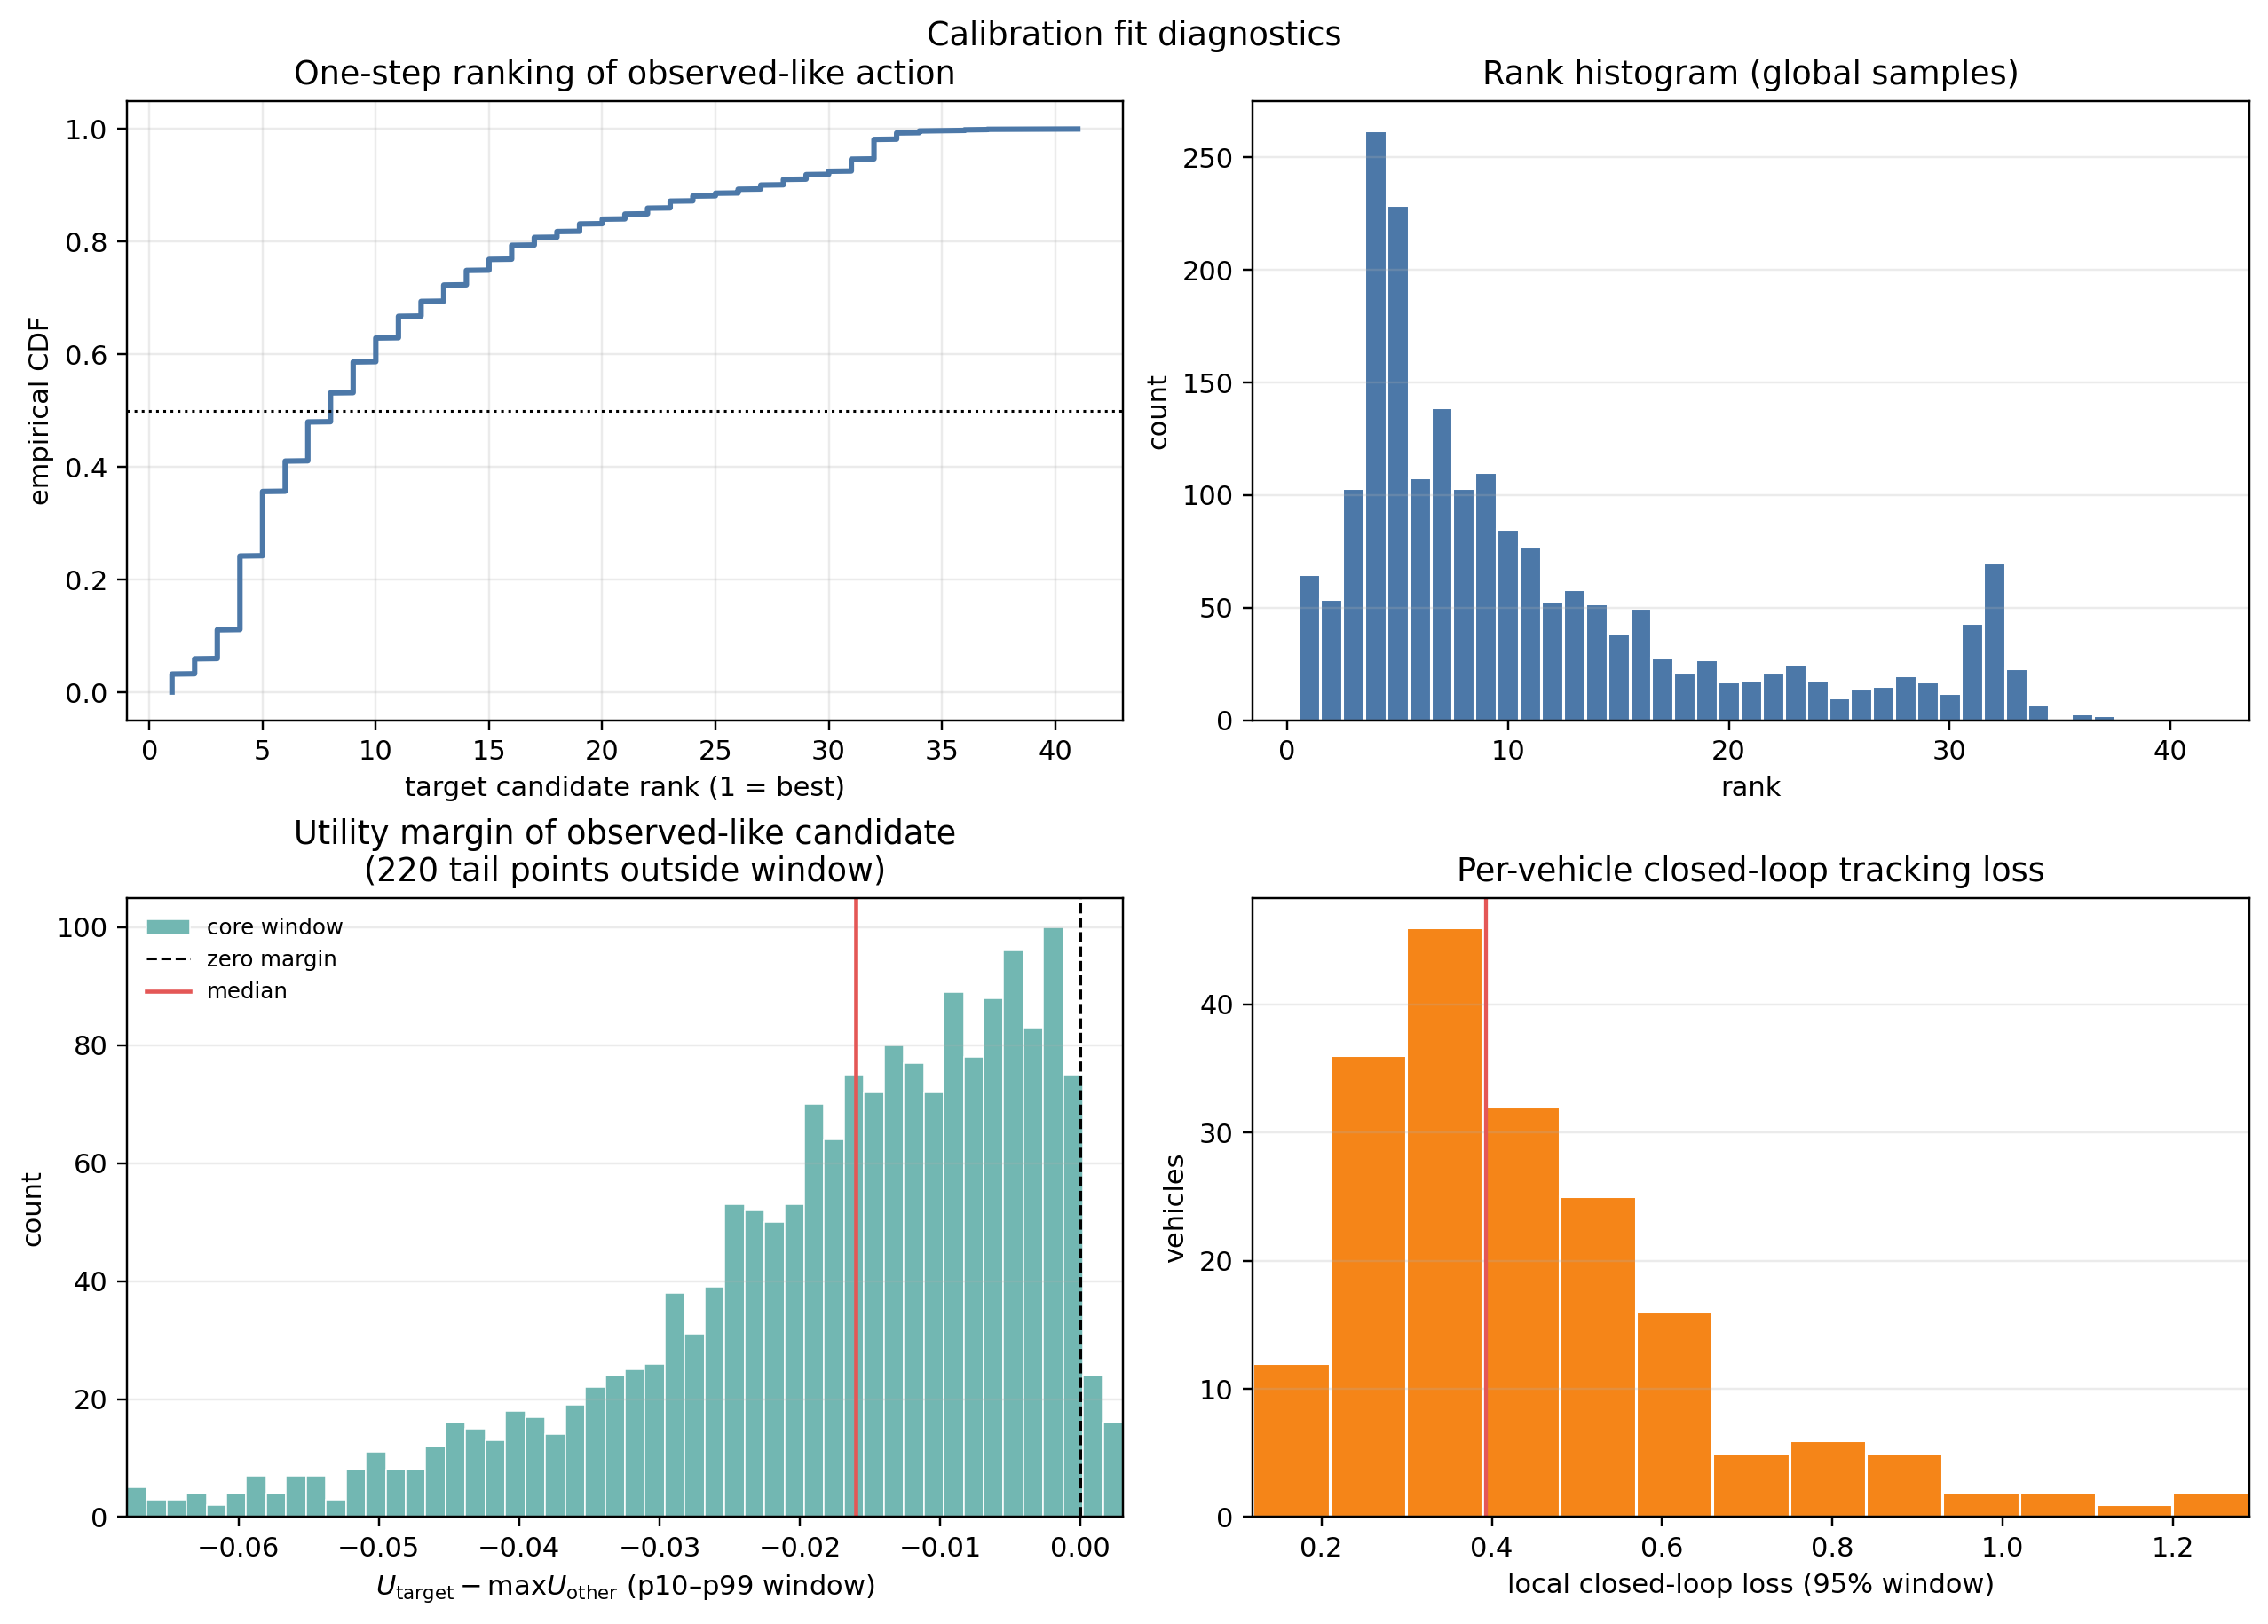
\includegraphics[width=0.95\linewidth]{Pics/fig_fit_quality.png}
\caption{Calibration fit diagnostics: empirical CDF and histogram of the observed-like candidate rank, utility margin relative to the best alternative (core p10--p99 window), and per-vehicle closed-loop tracking loss.}
\label{fig:calibration_fit_quality}
\end{figure*}

\paragraph{Working parameters and uncertainty.}
Table~\ref{tab:utility_calibration_params} reports the single best vector, the robust working point, and top-cloud percentiles after vehicle-scale collision-kernel recalibration. We recommend $\theta_{\mathrm{rob}}$ for all downstream simulation and residual learning:
\[
\begin{aligned}
&S_\theta=4.13,\ 
S_v=2.51,\ 
\xi_i=4.04,\ 
S_d=9.43,\ 
\gamma=0.56,\\
&w_x=4.85,\ 
w_y=5.83,\ 
w_c=300,\ 
w_\ell=77.6,\ 
\beta=2.14,\\
&\sigma_{\parallel}=0.89\,\mathrm{m},\ 
\sigma_{\perp}=0.59\,\mathrm{m}.
\end{aligned}
\]
Relative to $\theta^\star$, the robust set raises the weakly identified collision weight ($w_c$: $15\to 300$) and reduces an extreme path weight ($w_\ell$: $161\to 78$), while keeping metre-scale kernel widths consistent with passenger-car half-extents. Fig.~\ref{fig:calibration_param_dist} shows the global scored-trial distributions (histogram and KDE restricted to the central $95\%$ mass), and Fig.~\ref{fig:calibration_param_dist_per_id} reports the corresponding per-vehicle local-fit distributions.

\begin{figure*}[!t]
\centering
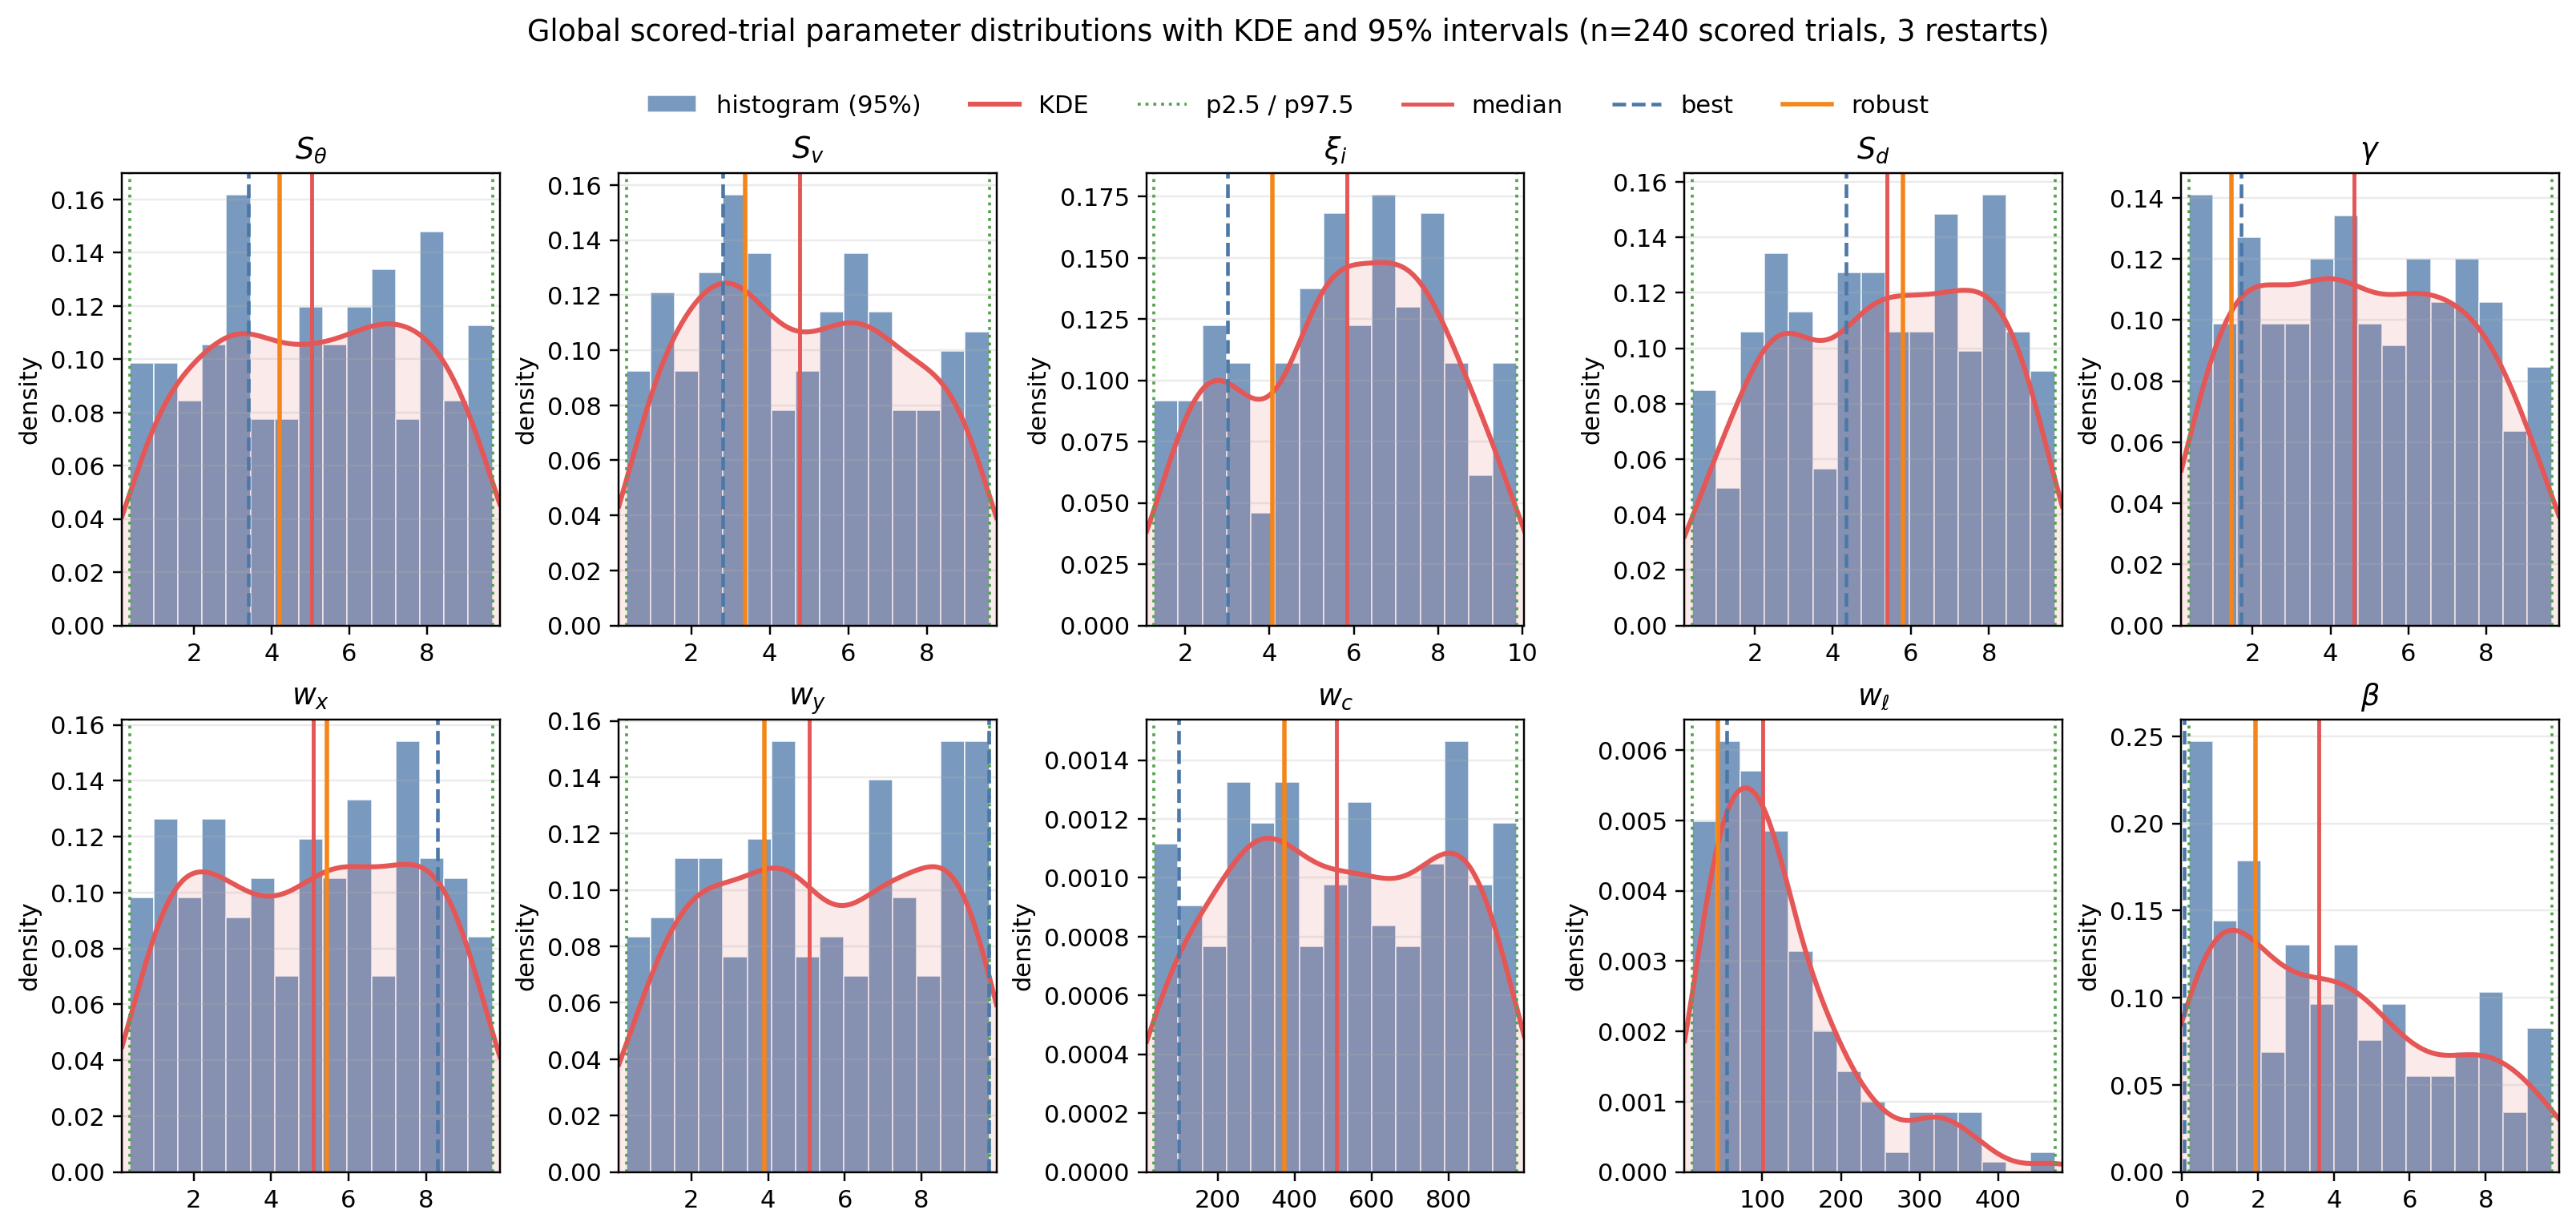
\includegraphics[width=\linewidth]{Pics/fig_parameter_distributions.png}
\caption{Global scored-trial distributions of the twelve utility parameters ($240$ closed-loop-scored trials from three restarts). Histograms and KDEs are computed inside each parameter's central $95\%$ interval; vertical markers indicate the median, best, and robust values when they fall in that window.}
\label{fig:calibration_param_dist}
\end{figure*}

\begin{figure*}[!t]
\centering
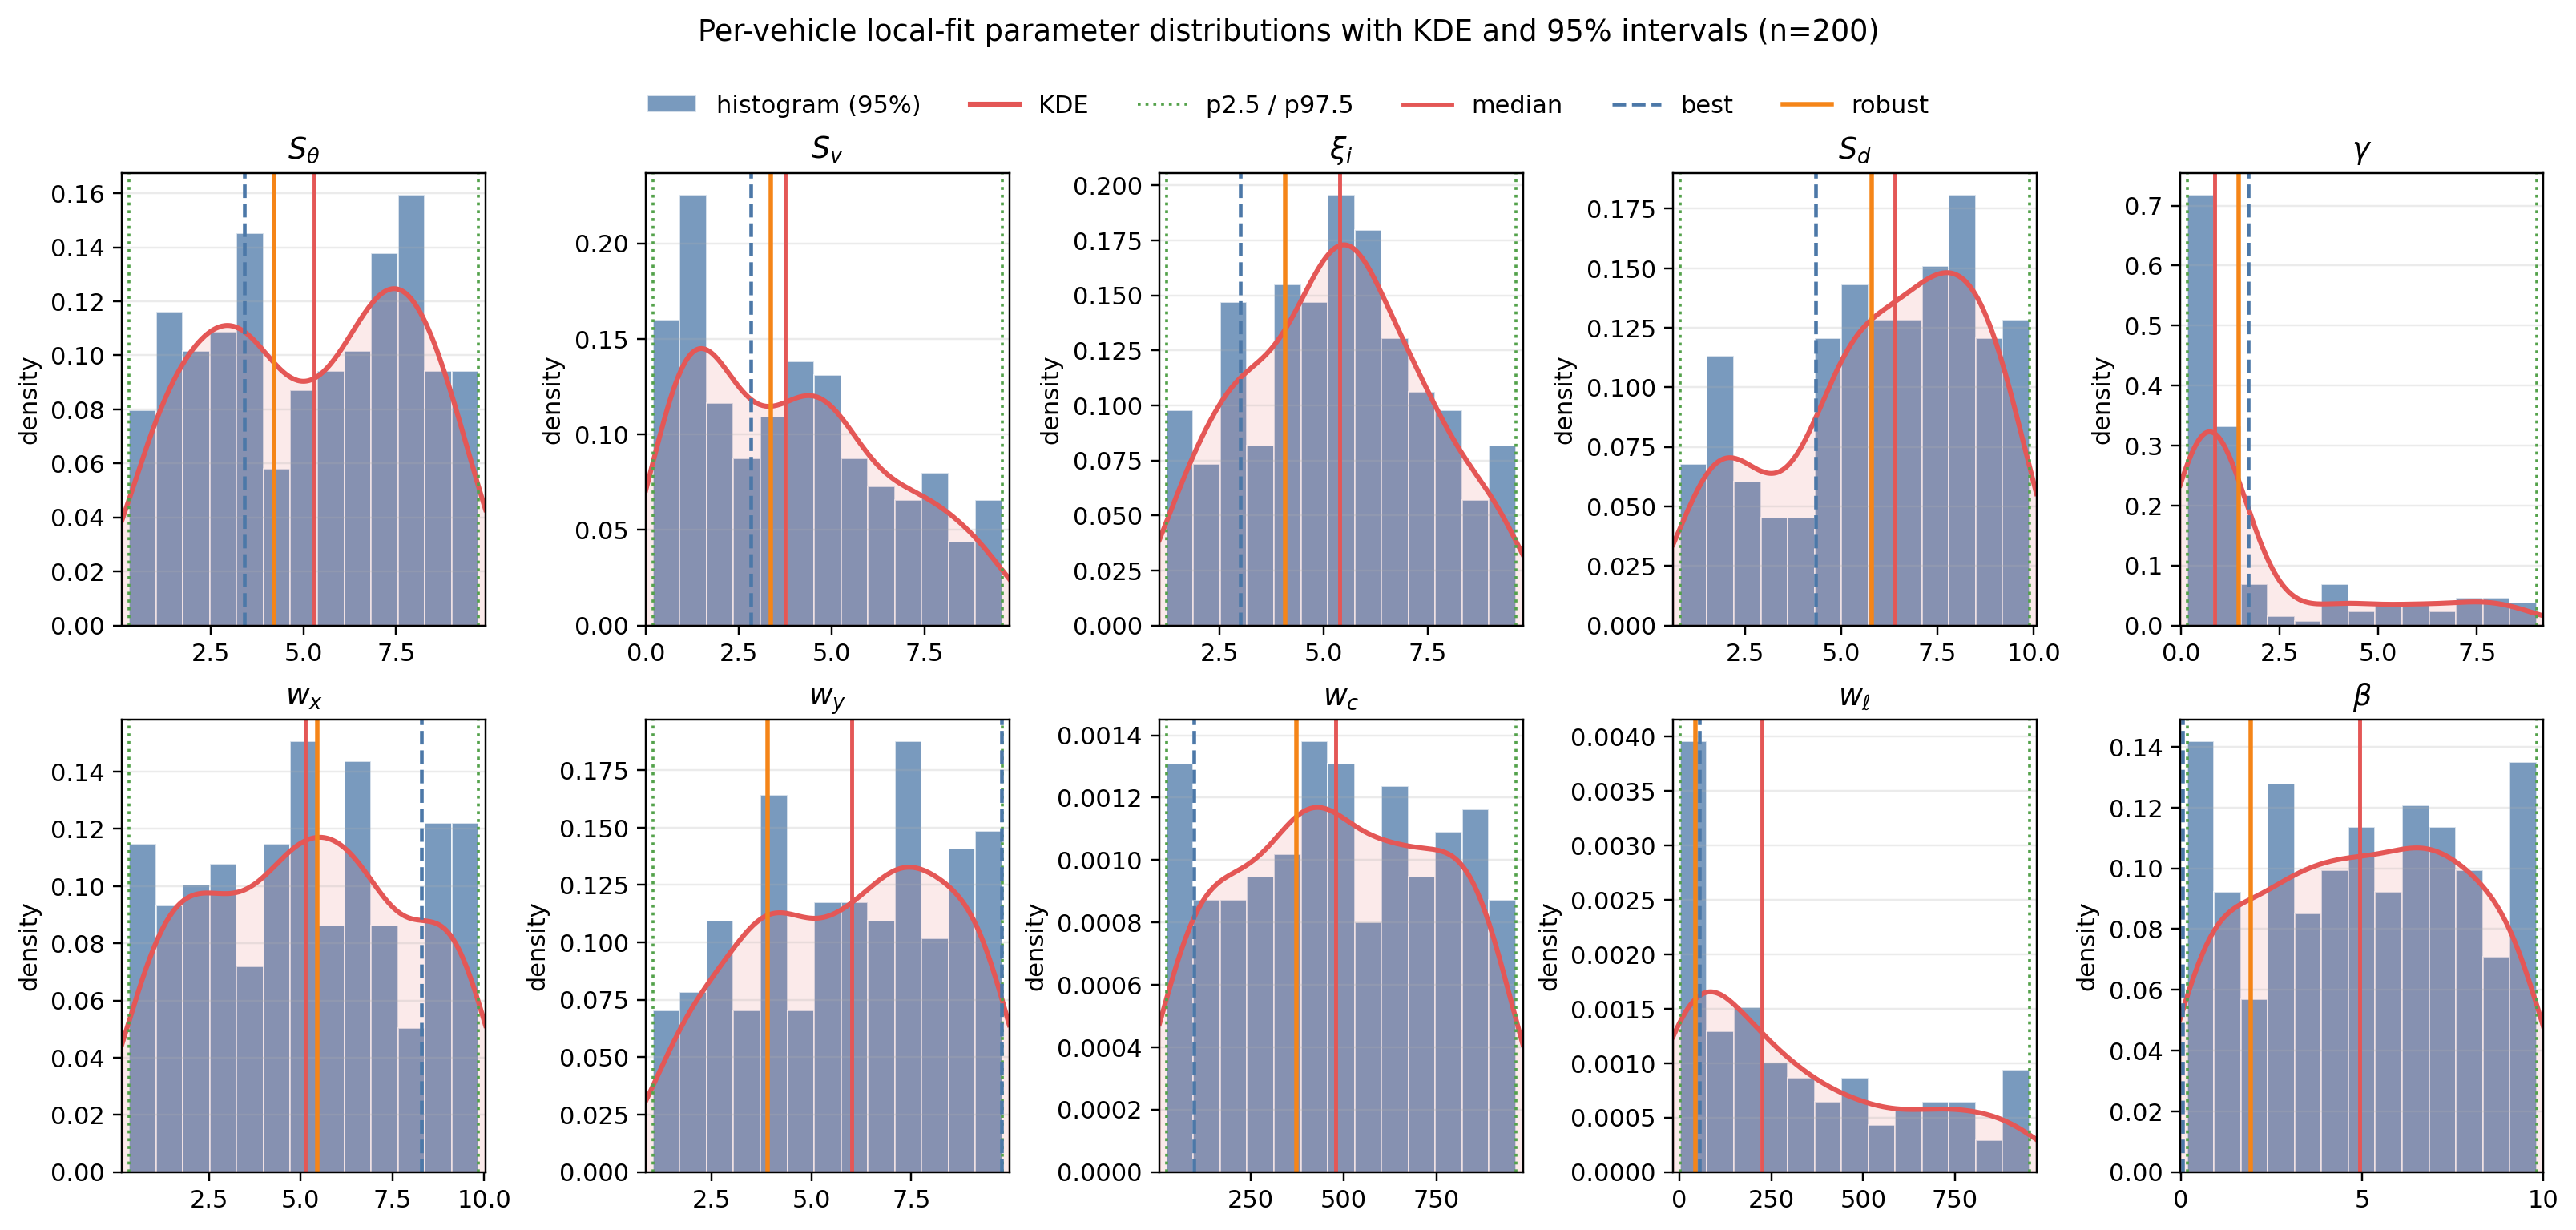
\includegraphics[width=\linewidth]{Pics/fig_parameter_distributions_per_id.png}
\caption{Per-vehicle local-fit parameter distributions ($200$ trajectories). Histograms and KDEs use the central $95\%$ mass for each coordinate.}
\label{fig:calibration_param_dist_per_id}
\end{figure*}

\paragraph{Identifiability.}
Of $240$ closed-loop-scored trials, only a small subset lies near $J(\theta^\star)$; the near-optimal/top cloud still exhibits large coefficient-of-variation across most coordinates (Fig.~\ref{fig:calibration_identifiability}). The strongest near-optimal tradeoff is between $S_v$ and $w_c$ (correlation $\approx 1$), with additional coupling among $(\gamma,w_x)$, $(w_c,\sigma_{\perp})$, and $(S_v,\sigma_{\perp})$. Thus the data identify a \emph{region} of acceptable utility weights more reliably than a unique point estimate.

\begin{figure*}[!t]
\centering
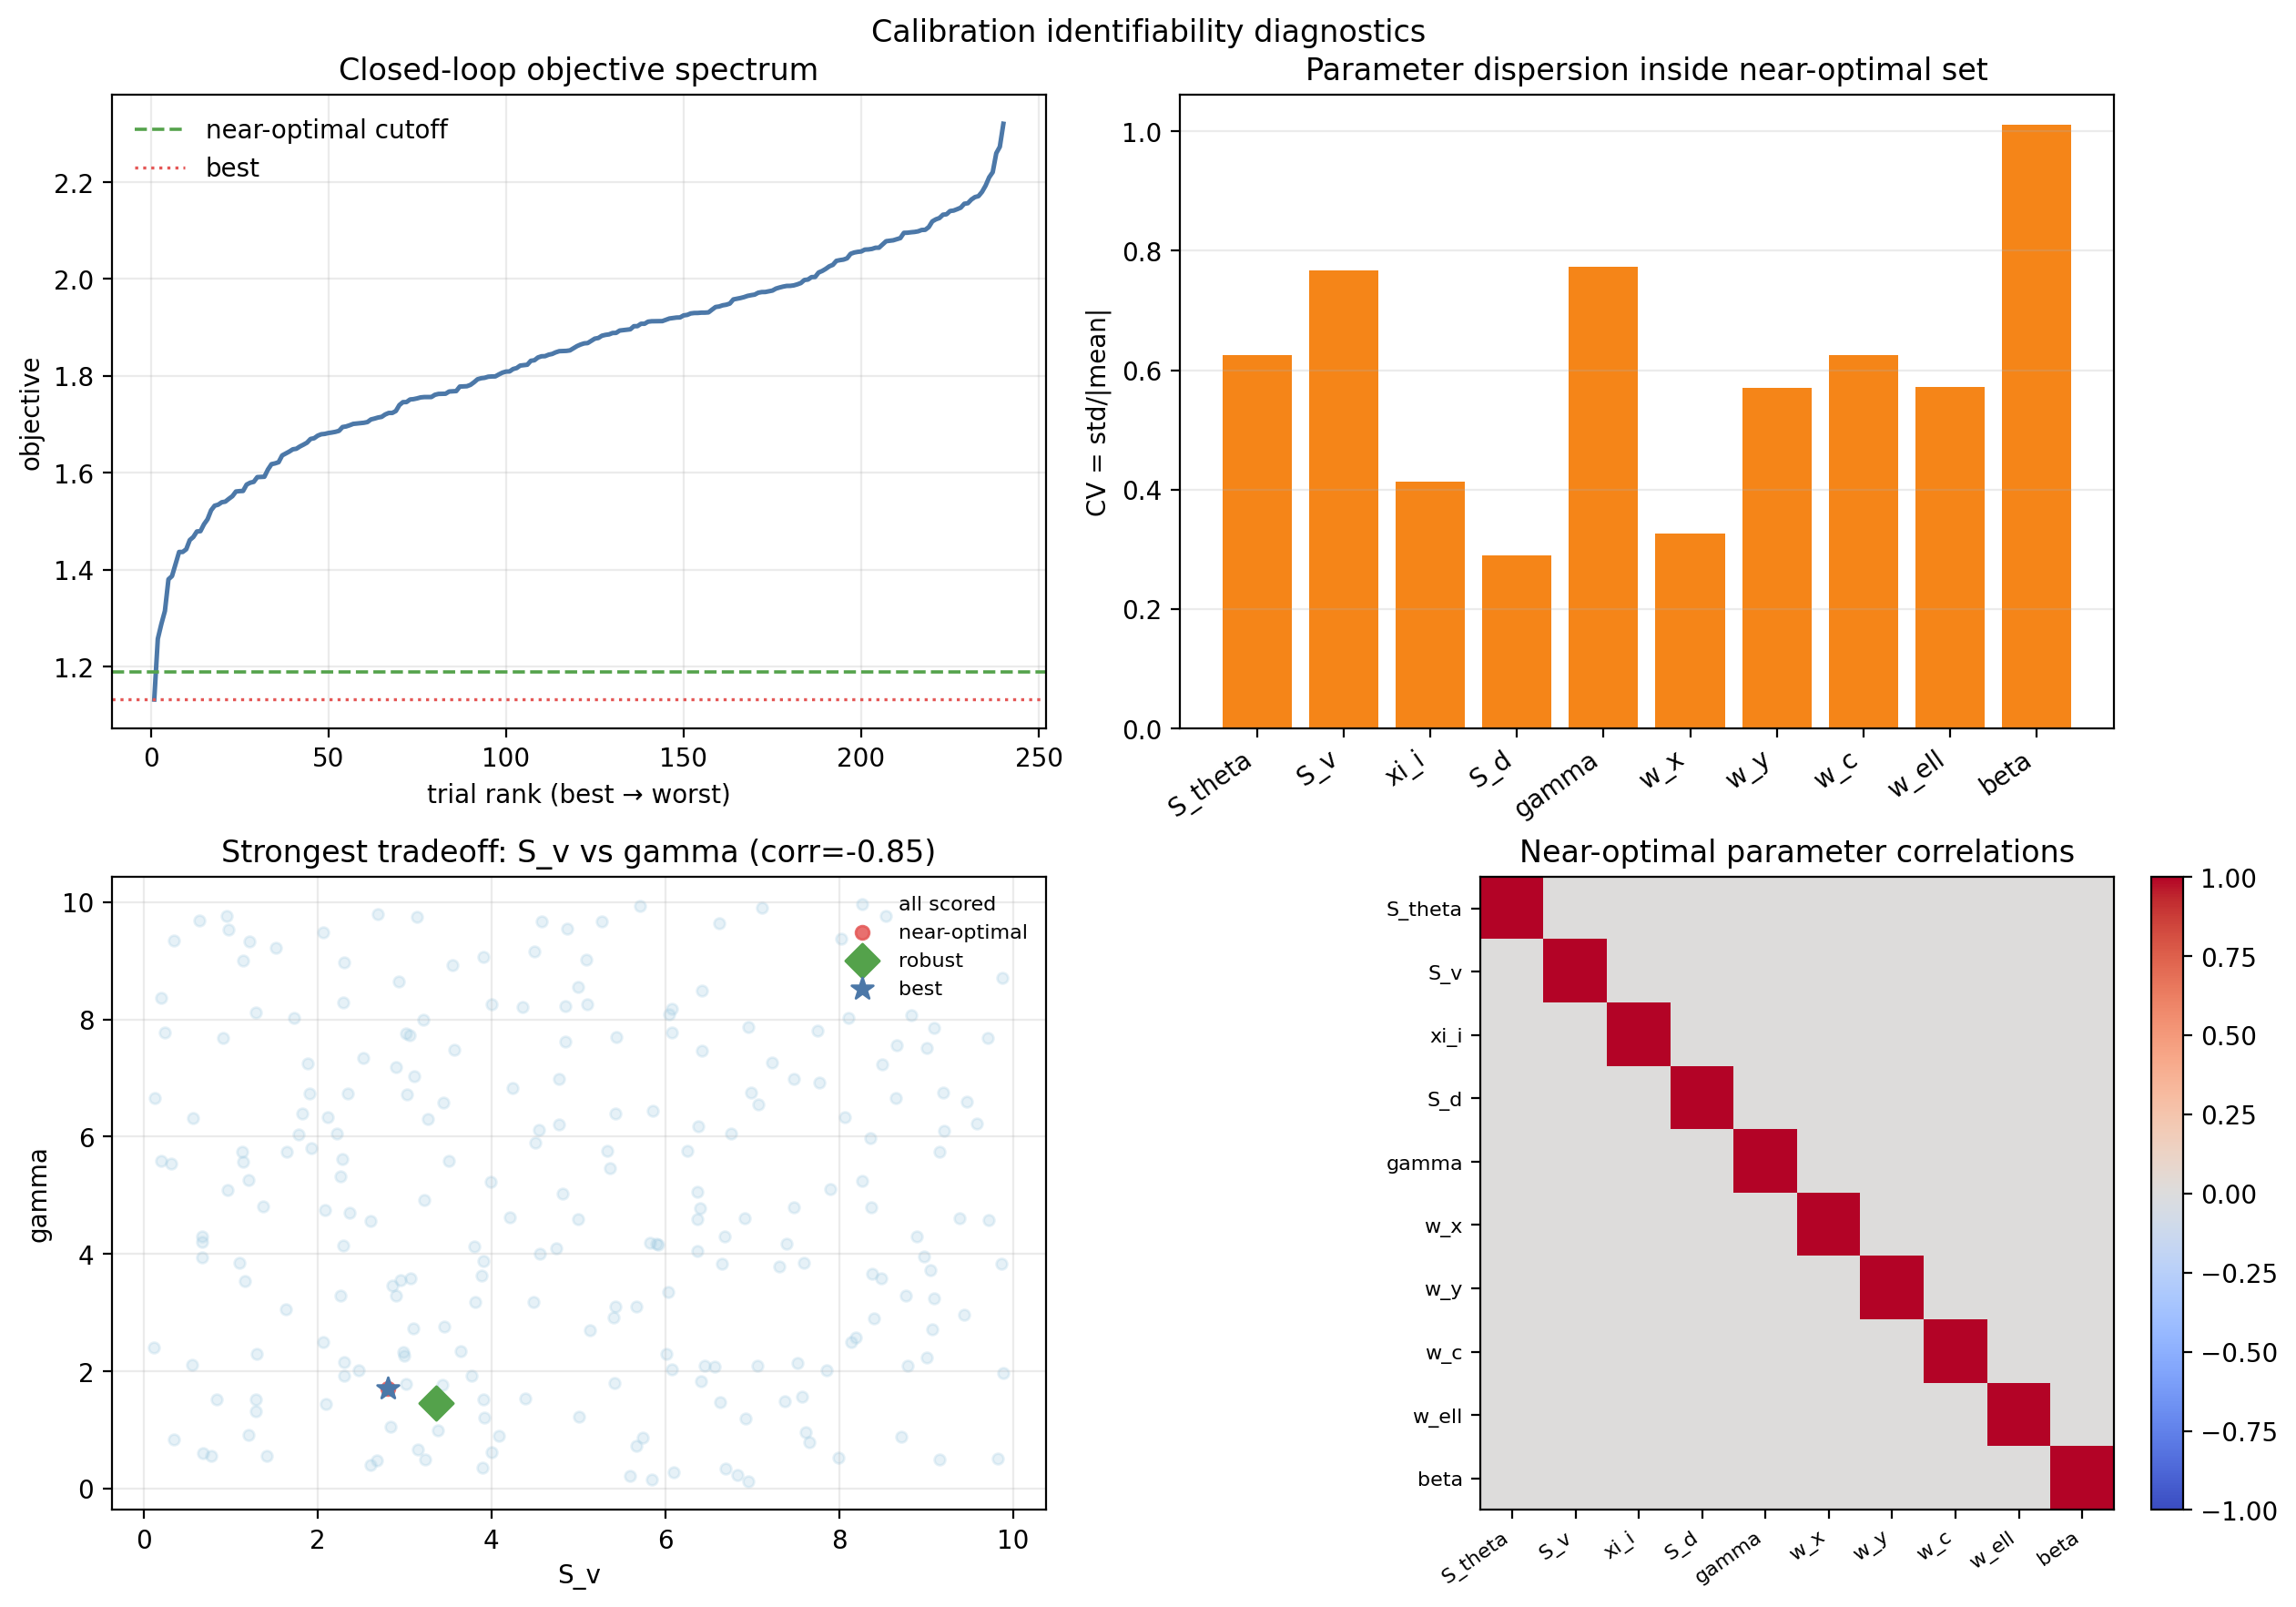
\includegraphics[width=0.95\linewidth]{Pics/fig_identifiability_diagnostics.png}
\caption{Identifiability diagnostics for the twelve-parameter freeway fit: pairwise tradeoffs in the near-optimal cloud (notably $S_v$--$w_c$) and coefficient-of-variation across coordinates.}
\label{fig:calibration_identifiability}
\end{figure*}

\paragraph{Implications.}
For the remainder of this paper we (i)~fix $\theta_{\mathrm{rob}}$ as the nominal utility prior, (ii)~treat the reported percentile ranges as the calibrated uncertainty region, and (iii)~interpret residual policy learning as refining behavior within an already plausible, but non-unique, utility basin. The appendix Sobol study predates this region and is not computed on these percentiles.

\begin{table*}[!t]
\centering
\caption{Calibrated utility parameters after vehicle-scale collision-kernel recalibration: best trial, robust median of the near-optimal cloud, and top-cloud $p_{50}$/$p_{95}$.}
\label{tab:utility_calibration_params}
\begin{tabular}{lrrrrr}
\toprule
Param. & Best & Robust & Top $p_{50}$ & Top $p_{95}$ \\
\midrule
$S_\theta$ & $6.744$ & $4.126$ & $5.860$ & $9.147$ \\
$S_v$      & $0.989$ & $2.512$ & $2.666$ & $8.522$ \\
$\xi_i$    & $2.318$ & $4.036$ & $4.785$ & $8.989$ \\
$S_d$      & $9.908$ & $9.432$ & $6.181$ & $9.723$ \\
$\gamma$   & $0.388$ & $0.563$ & $3.164$ & $8.211$ \\
$w_x$      & $3.079$ & $4.853$ & $6.556$ & $9.798$ \\
$w_y$      & $9.593$ & $5.833$ & $4.214$ & $9.503$ \\
$w_c$      & $15.12$ & $299.7$ & $255.0$ & $678.9$ \\
$w_\ell$   & $161.5$ & $77.64$ & $36.42$ & $135.3$ \\
$\beta$    & $2.142$ & $2.142$ & $4.488$ & $8.812$ \\
$\sigma_{\parallel}$ (m) & $0.889$ & $0.889$ & $2.310$ & $4.574$ \\
$\sigma_{\perp}$ (m) & $1.338$ & $0.593$ & $1.385$ & $2.020$ \\
\bottomrule
\end{tabular}
\end{table*}

\section{Experimental Setup for Residual Learning and Benchmarking}
\label{sec:rl_setup}

All residual-learning and baseline comparisons use a shared closed-loop harness on the Lebanon freeway corridor (\texttt{run\_id}$=2$, lane Kalman filter branch $1$). Agents are integrated with the kinematic bicycle model, collisions are detected with oriented bounding boxes (OBBs), and corridor feasibility is enforced in Frenet coordinates. Scenario seeds, spawn windows, and episode lengths are matched across models so that differences reflect controllers rather than initialization.

\paragraph{Residual training.}
The utility prior is frozen at the robust calibrated vector $\Theta_{\mathrm{base}}=\theta_{\mathrm{rob}}$ (Table~\ref{tab:utility_calibration_params}). A shared-policy PPO residual agent outputs the nine-dimensional $\Delta\Theta$ defined above (including collision-kernel scales $(\Delta\sigma_{\parallel},\Delta\sigma_{\perp})$). Observations are fully decentralized Frenet/body-frame features. Rewards follow Eqs.~\eqref{eq:R_progress}--\eqref{eq:R_boundary}, with contact-aware safety, a per-contact OBB penalty, and a depth-capped off-road term. Closed-loop utility evaluation uses the $1.5\,\mathrm{s}$ OBB lookahead described above. Unless noted, residual checkpoints are trained under the sparse protocol below.

\paragraph{Benchmark models.}
The paper-facing comparison set is: ORCA, social force, dynamic window approach (DWA), model-predictive path-integral control (MPPI), MAPPO (pure MARL without a utility prior, retrained on the same Frenet/body-frame observations), the calibrated utility prior, and residual MARL. A Frenet lattice planner and alternative MARL variants (IPPO, HAPPO, HATRPO) remain negative controls (poor arrival/safety trade-offs or unstable returns).

\paragraph{Metrics.}
We report mean collision events per episode, off-road rate, arrival rate, travel time, RMS jerk, and a realism score defined as the mean 1-D Wasserstein distance between simulated and measured marginals of speed, longitudinal acceleration, and lateral offset (lower is more human-like). Minimum TTC and related safety auxiliaries are logged but not emphasized in the main table.

\paragraph{Protocols.}
The paper's target use case is dense spatial negotiation with human-like kinematics, not sparse geometric collision avoidance. \emph{Sparse:} $10$ scenarios $\times$ $10$ agents with the default spawn window. \emph{Ablation:} the same seeds comparing the prior, residual MARL, and a $\sigma$-frozen residual (kernel scales clamped to $\Theta_{\mathrm{base}}$). \emph{Dense stress:} $18$ agents with a tighter spawn window on the same corridor.

\section{Residual MARL Results}
\label{sec:residual_results}

Residual MARL is evaluated first against the frozen utility prior it is designed to improve, then against unconstrained MAPPO, and then against a kernel-scale ablation that tests the contribution of $(\Delta\sigma_{\parallel},\Delta\sigma_{\perp})$.

Under the sparse protocol (Table~\ref{tab:ablation}), vehicle-scale OBB lookahead saturates pairwise safety for the entire utility family: the prior, residual MARL, and the $\sigma$-frozen residual all record $0.0$ mean collisions. Residual MARL is not a sparse collision-avoidance win over the prior; it is a throughput win inside that collision-free band, raising arrival from $0.86$ to $0.89$ with comparable travel time. Freezing kernel-scale residuals returns arrival to the prior's $0.86$ and slightly increases RMS jerk ($5.35$ versus $5.03$). MAPPO is the sparse speed leader (travel time $33.8\,\mathrm{s}$, arrival $0.93$) but records $2.1$ collisions and a worse realism score ($0.940$ versus residual $0.822$). Social force edges MAPPO on sparse arrival ($0.94$) while still colliding ($0.3$).

The dense protocol (Table~\ref{tab:stress}) is the remaining discriminator. Mean utility-family collisions fall from $8.5$ (prior) to $7.1$ (residual; $\Delta=-1.4$), while the $\sigma$-frozen residual sits at $8.9$. MAPPO's sparse arrival advantage transfers as speed, not safety: collisions rise to $44.9$ with $0.97$ arrival and $15.1\,\mathrm{m/s}$ mean speed. The residual collision $\Delta$ versus the prior is not statistically significant at $n=10$ ($p\approx 0.44$), whereas residual RMS jerk is lower ($6.16$ versus $6.76$). Residual off-road rate increases ($0.32$ versus $0.24$). Kernel adaptation still helps contacts under crowding relative to the prior and is far safer than unconstrained MAPPO, but it is not a free lunch on corridor compliance.

\begin{table}[!t]
\centering
\caption{Sparse matched-seed ablation ($10$ scenarios $\times$ $10$ agents). Collisions are mean events per episode. Lookahead saturates safety for the utility family; residual MARL raises arrival relative to the prior, and kernel freezing removes that throughput gain.}
\label{tab:ablation}
\begin{tabular}{lcccc}
\toprule
Model & Collisions & Arrival & Travel (s) & Jerk \\
\midrule
Utility prior & 0.0 & 0.86 & 59.3 & 4.96 \\
Residual MARL & 0.0 & 0.89 & 60.2 & 5.03 \\
Residual ($\sigma$ frozen) & 0.0 & 0.86 & 59.6 & 5.35 \\
MAPPO & 2.1 & 0.93 & 33.8 & 0.63 \\
\bottomrule
\end{tabular}

\end{table}

\begin{table}[!t]
\centering
\caption{Dense stress protocol ($18$ agents, tighter spawn; mean over $10$ scenarios). Residual MARL lowers mean collisions relative to the prior; unconstrained MAPPO keeps arrival by colliding.}
\label{tab:stress}
\begin{tabular}{lcccc}
\toprule
Model & Collisions & Arrival & Travel (s) & Jerk \\
\midrule
Utility prior & 8.5 & 0.90 & 55.9 & 6.76 \\
Residual MARL & 7.1 & 0.91 & 56.6 & 6.16 \\
Residual ($\sigma$ frozen) & 8.9 & 0.92 & 56.4 & 6.57 \\
MAPPO & 44.9 & 0.97 & 34.6 & 0.64 \\
\bottomrule
\end{tabular}

\end{table}

\begin{figure}[!t]
\centering
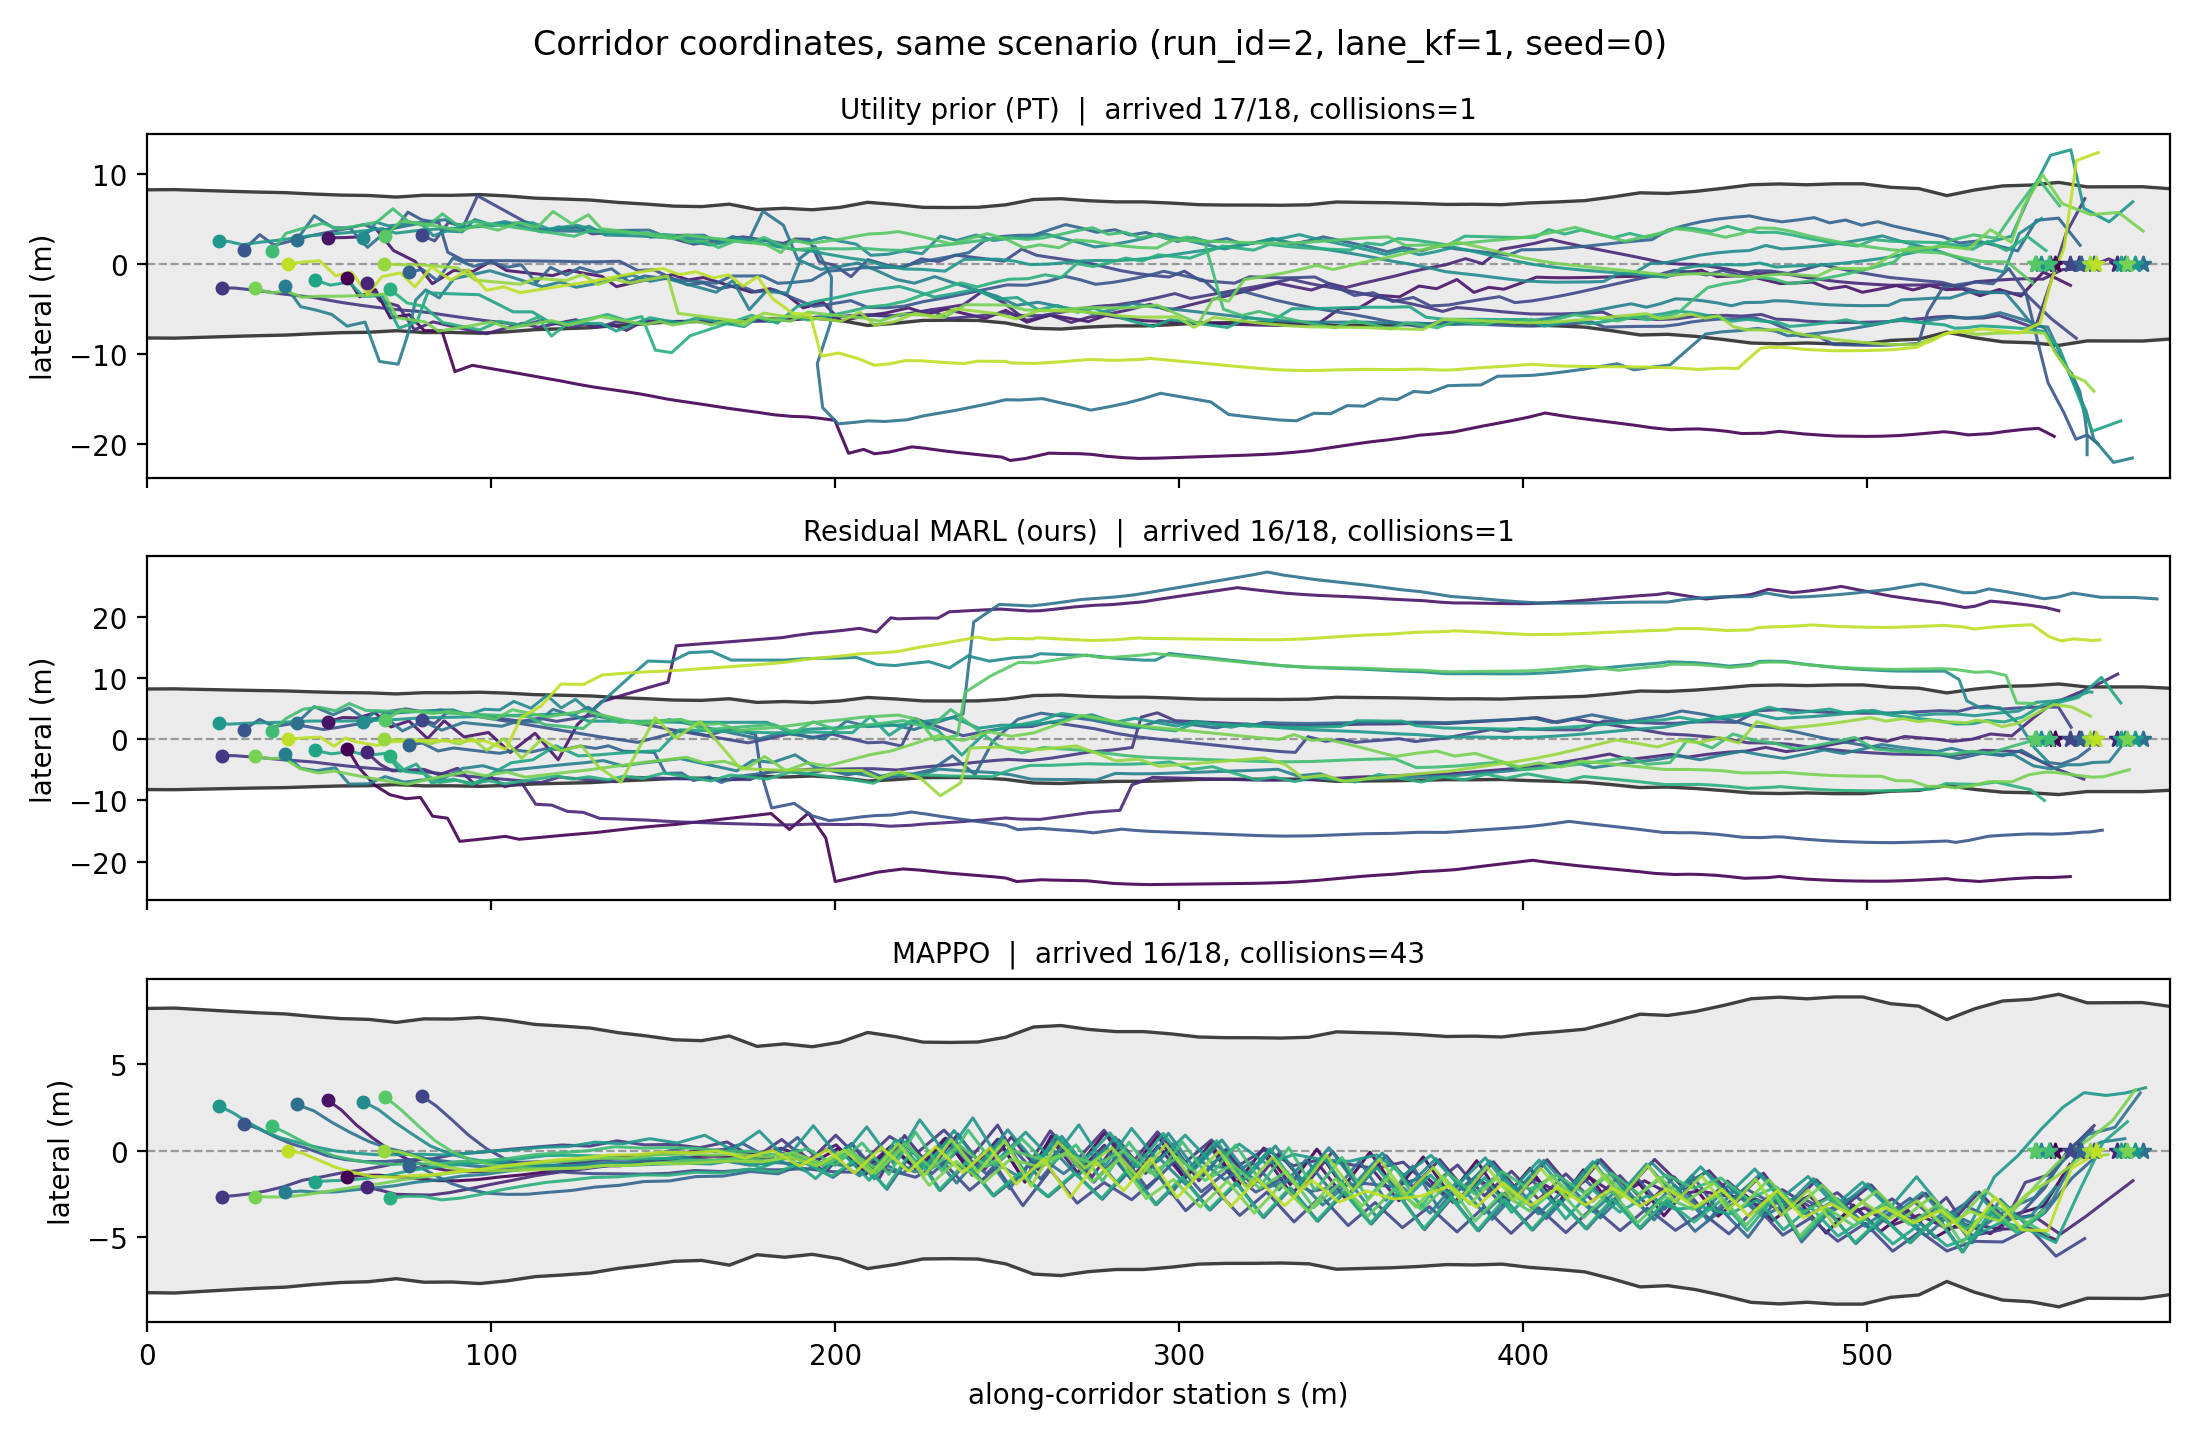
\includegraphics[width=0.95\linewidth]{Pics/fig_stress_frenet.png}
\caption{Dense $18$-agent Frenet packing on a matched seed. Residual MARL stays near the prior's contact count; unconstrained MAPPO packs by colliding.}
\label{fig:stress_frenet}
\end{figure}

\section{Benchmark}
\label{sec:benchmark}

Table~\ref{tab:benchmark_main} reports the seven-model sparse protocol. With $1.5\,\mathrm{s}$ vehicle-scale OBB lookahead \emph{inside the utility kernel}, the calibrated prior and residual MARL are collision-free. MAPPO records $2.1$ contacts with the shortest travel time ($33.8\,\mathrm{s}$; arrival $0.93$). Social force has a slightly higher sparse arrival ($0.94$) while still colliding ($0.3$). Pairwise geometric planners still record residual contacts: social force $0.3$, ORCA/DWA $0.5$, and MPPI $3.2$. That comparison is intentional rather than a claim that planners cannot avoid collisions: they optimize their native geometric costs, not the lookahead-equipped utility. Residual MARL has the highest arrival among collision-free controllers ($0.89$ versus the prior's $0.86$).

Among models that \emph{are} intended as behavioral generators, residual MARL slightly improves the prior's realism score ($0.822$ versus $0.836$; lower is closer to measured marginals) with comparable travel time. MAPPO's realism score ($0.940$) is worse, consistent with a high-speed policy (mean $14.8\,\mathrm{m/s}$ versus about $8.3$--$8.5$ for the utility family). The same Wasserstein column does \emph{not} rank residual above DWA/MPPI ($0.614$--$0.640$): those planners are smoother (RMS jerk $\approx 0.8$--$3.7$ versus $\approx 5$ for the utility family) and can match speed/acceleration/lateral \emph{marginals} without matching observed discrete choice. We therefore treat realism as a check that residual stays in the prior's distributional band, not as a claim that the generator is more human-like than a geometric oracle.

Fig.~\ref{fig:benchmark_metrics} summarizes the sparse metric panel. Fig.~\ref{fig:realism_panel} shows simulated versus measured speed, acceleration, and lateral-offset distributions. Fig.~\ref{fig:stress_frenet} illustrates packing on the dense protocol, whose numeric ranking is reported in Table~\ref{tab:stress}. Combined, the sparse and dense comparisons support three statements:
\begin{itemize}
    \item residual MARL improves a calibrated human prior without leaving the interpretable utility maximizer;
    \item unconstrained MAPPO wins travel time by speeding, then loses safety under crowding ($44.9$ dense collisions versus residual $7.1$);
    \item geometric planners remain geometric: they optimize avoidance, not observed choice.
\end{itemize}

\begin{table*}[!t]
\centering
\caption{Main sparse diagnostic on the Lebanon freeway corridor ($10$ scenarios $\times$ $10$ agents; mean $\pm$ std across scenarios). Realism is mean Wasserstein distance to measured speed/acceleration/lateral marginals (lower is better). MAPPO is unconstrained MARL; residual MARL is the proposed behavioral generator.}
\label{tab:benchmark_main}
\begin{tabular}{lcccccc}
\toprule
Model & Coll. & Off-road & Arrival & Travel (s) & Jerk & Realism $\downarrow$ \\
\midrule
ORCA & 0.50 $\pm$ 0.92 & 0.002 $\pm$ 0.005 & 0.850 $\pm$ 0.112 & 63.8 $\pm$ 3.9 & 0.79 $\pm$ 0.10 & 0.720 $\pm$ 0.046 \\
Social force & 0.30 $\pm$ 0.64 & 0.000 $\pm$ 0.000 & 0.940 $\pm$ 0.049 & 66.8 $\pm$ 3.2 & 0.77 $\pm$ 0.07 & 0.704 $\pm$ 0.031 \\
DWA & 0.50 $\pm$ 0.92 & 0.000 $\pm$ 0.000 & 0.850 $\pm$ 0.102 & 60.0 $\pm$ 1.4 & 3.66 $\pm$ 0.15 & 0.640 $\pm$ 0.028 \\
MPPI & 3.20 $\pm$ 2.44 & 0.000 $\pm$ 0.000 & 0.580 $\pm$ 0.204 & 60.5 $\pm$ 3.3 & 1.50 $\pm$ 0.21 & 0.614 $\pm$ 0.090 \\
MAPPO & 2.10 $\pm$ 2.84 & 0.000 $\pm$ 0.000 & 0.930 $\pm$ 0.078 & 33.8 $\pm$ 0.5 & 0.63 $\pm$ 0.07 & 0.940 $\pm$ 0.038 \\
Utility prior & 0.00 $\pm$ 0.00 & 0.007 $\pm$ 0.011 & 0.860 $\pm$ 0.080 & 59.3 $\pm$ 3.3 & 4.96 $\pm$ 1.32 & 0.836 $\pm$ 0.163 \\
Residual MARL (ours) & 0.00 $\pm$ 0.00 & 0.007 $\pm$ 0.007 & 0.890 $\pm$ 0.083 & 60.2 $\pm$ 3.7 & 5.03 $\pm$ 1.12 & 0.822 $\pm$ 0.124 \\
\bottomrule
\end{tabular}
\end{table*}

\begin{figure*}[!t]
\centering
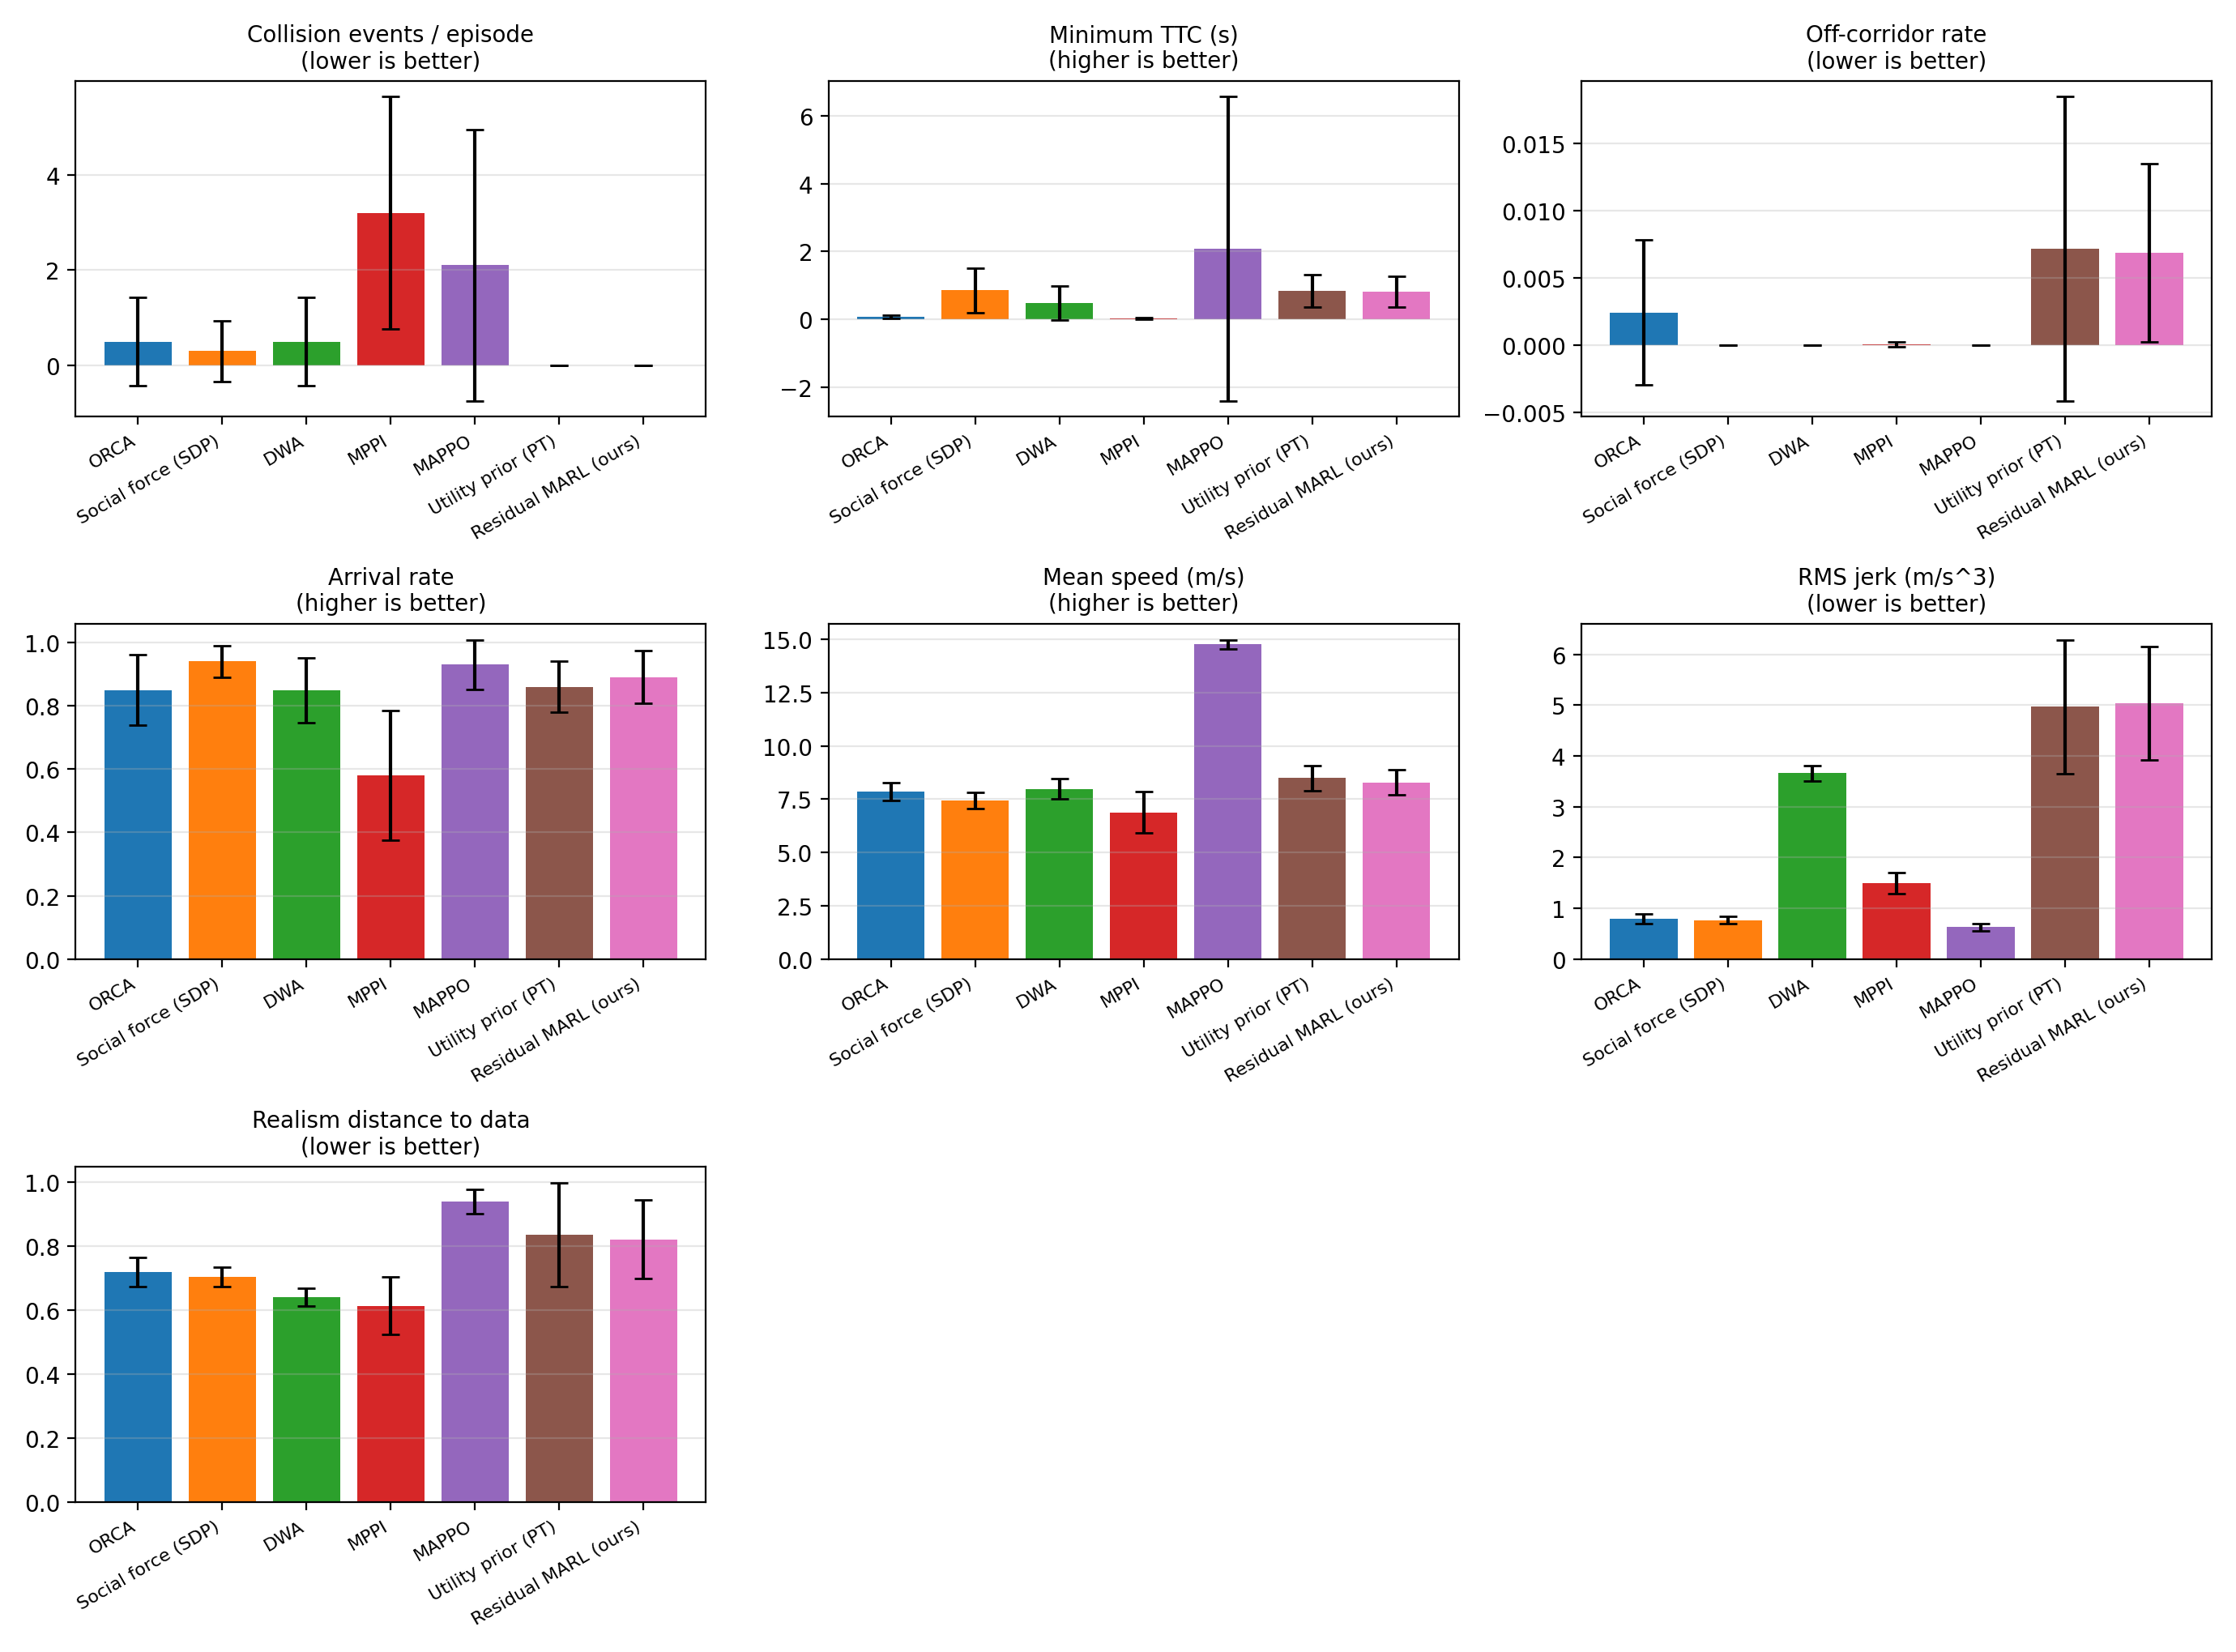
\includegraphics[width=0.95\linewidth]{Pics/fig_benchmark_metrics.png}
\caption{Sparse protocol metric panel including MAPPO. With OBB lookahead the calibrated prior and residual MARL are collision-free; MAPPO is the speed outlier.}
\label{fig:benchmark_metrics}
\end{figure*}

\begin{figure*}[!t]
\centering
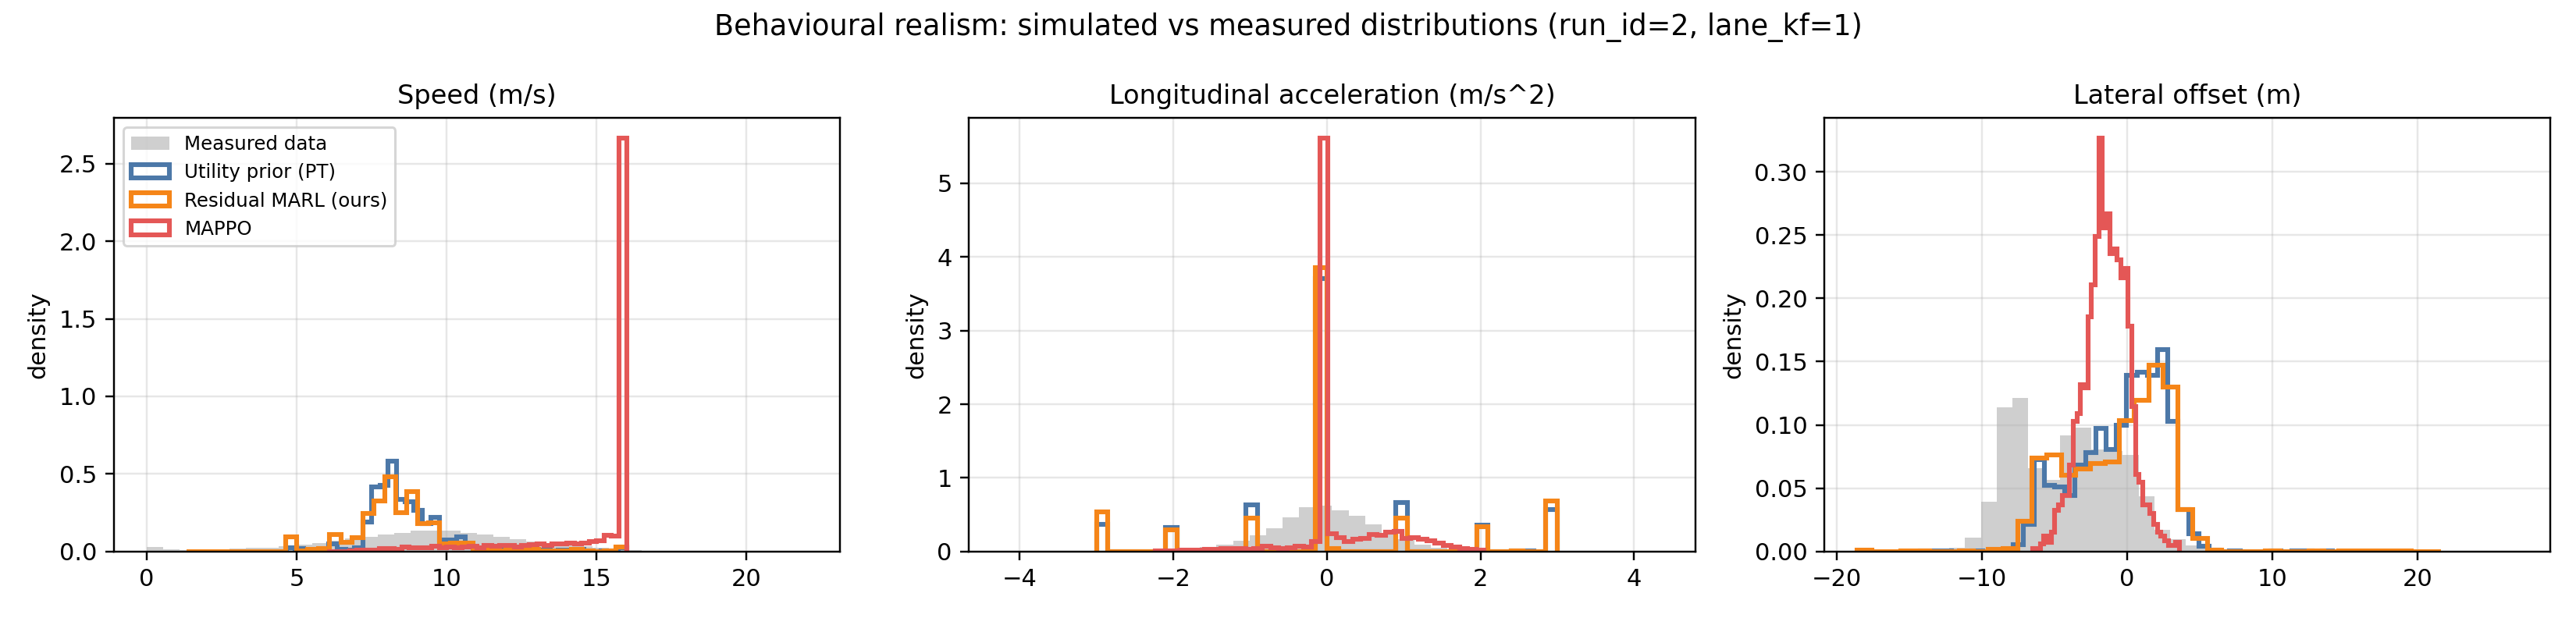
\includegraphics[width=0.85\linewidth]{Pics/fig_realism_panel.png}
\caption{Realism panel: measured versus simulated speed, acceleration, and lateral-offset marginals. Residual MARL stays in the prior's distributional band; MAPPO's speed mass sits well above the measured mode.}
\label{fig:realism_panel}
\end{figure*}

\section{Conclusion}
\label{sec:conclusion}

We presented a utility-guided residual MARL framework for decentralized motion on a weak-lane freeway corridor. After calibrating a twelve-parameter utility prior with vehicle-scale collision kernels, a shared residual policy learns nine-dimensional parameter adjustments---including kernel scales---rather than raw controls. On the sparse freeway protocol, OBB lookahead already makes the calibrated prior collision-free; residual MARL then raises arrival from $0.86$ to $0.89$ without adding contacts. MAPPO is faster (arrival $0.93$, $33.8\,\mathrm{s}$) but collides ($2.1$). Under denser spawn, residual mean collisions are $7.1$ versus the prior's $8.5$ and MAPPO's $44.9$; freezing $\Delta\sigma$ returns $8.9$. These results support residual utility adaptation as a practical route to context-dependent negotiation without abandoning interpretable behavioral structure.

\section{Limitations}
In calibration, although the calibrated utility prior provides a usable working point for residual learning, several limitations should be noted. First, the twelve-dimensional utility parameter vector is only weakly identified: multiple substantially different parameter combinations attain nearly the same closed-loop objective, with strong tradeoffs such as that between \(S_v\) and \(w_c\). Consequently, the calibration identifies a region of acceptable behavior rather than a unique optimum, which is why we report a robust median of near-optimal trials together with percentile ranges instead of relying on a single best vector. Second, one-step ranking remains imperfect on the discrete candidate grid---the observed-like action is frequently competitive (mean rank about six) but is rarely selected as the unique maximizer---so the one-step likelihood alone under-constrains the parameters and must be complemented by short-horizon closed-loop tracking. Third, per-vehicle local fits exhibit wide dispersion, indicating residual heterogeneity that a single population prior cannot fully capture. Finally, global sensitivity conclusions are meaningful only when Sobol ranges are aligned with the calibrated uncertainty region; using substantially narrower ad-hoc bounds can understate (or misattribute) parameter influence relative to the operating regime used downstream.

\paragraph{Residual learning and benchmarking.}
Closed-loop residual and baseline evaluations are freeway-only; residual transfer to the roundabout and Foggy Bottom priors is left for future work. Alternative MARL algorithms (IPPO, HAPPO, HATRPO) exhibited reward hacking or unstable returns in this harness and are not competitive paper baselines. MAPPO was retrained on the current Frenet observations (80 PPO updates, collision penalty $8$); it is a single training seed. Dense collision-penalty residual training was not completed for this draft. The dense residual collision improvement ($8.5$ to $7.1$) is modest and not significant at $n=10$ scenarios, and residual off-road rate is higher than the prior under crowding.

\bibliographystyle{IEEEtran} 
\bibliography{example}

\clearpage

\appendices
\section{Sensitivity Analysis}

Understanding parameter sensitivity is crucial to ensure that the agent-based model produces reliable, realistic, and robust behavior under a wide range of conditions \cite{chandler1958traffic, talebpour2011multiregime}. The sensitivity analysis reveals how robust the model is to parameter variations and helps guide parameter tuning.

To systematically assess model robustness, we perform both local and global sensitivity analyses. Local analysis examines the effect of small variations in individual parameters on each component of the utility function, providing insight into immediate system responsiveness. Global analysis, using techniques such as Sobol indices, quantifies the contribution of each parameter---including interactions---across their entire plausible range. Together, these analyses reveal how sensitive the model is to parameter changes and guide informed tuning for reliable and realistic agent behavior.

\section{Local Sensitivity Analysis}

Local sensitivity analysis quantifies how small parameter perturbations affect each component of the utility. We analyze the five utility terms from Equation~\ref{eq:utility}---directional alignment, speed incentive, proximity incentive, collision penalty, and path adherence---separately.

\subsection*{Directional Alignment}
Directional utility rewards candidate motion aligned with the local corridor tangent rather than a destination heading. Let \(\hat{m}\) denote the unit move direction induced by a candidate next position and \(\hat{t}\) the local corridor unit tangent. Then
\begin{equation}
\label{eq:Udir}
U_{\mathrm{dir}}
= S_{\theta}\,(\hat{m}\cdot\hat{t}).
\end{equation}
\begin{equation}
\label{eq:dUdir_dStheta}
\frac{\partial U_{\mathrm{dir}}}{\partial S_{\theta}}
= \hat{m}\cdot\hat{t}.
\end{equation}
\begin{equation}
\label{eq:dUdir_dalignment}
\frac{\partial U_{\mathrm{dir}}}{\partial (\hat{m}\cdot\hat{t})}
= S_{\theta}.
\end{equation}

Thus \(S_{\theta}\) linearly scales the directional reward. Utility is maximized when \(\hat{m}\cdot\hat{t}=1\) (perfect corridor alignment) and becomes negative when the candidate move opposes the corridor orientation. This remains valid for both positive- and negative-direction traffic because directionality is defined by corridor geometry.

\begin{figure}[htbp]
    \centering
    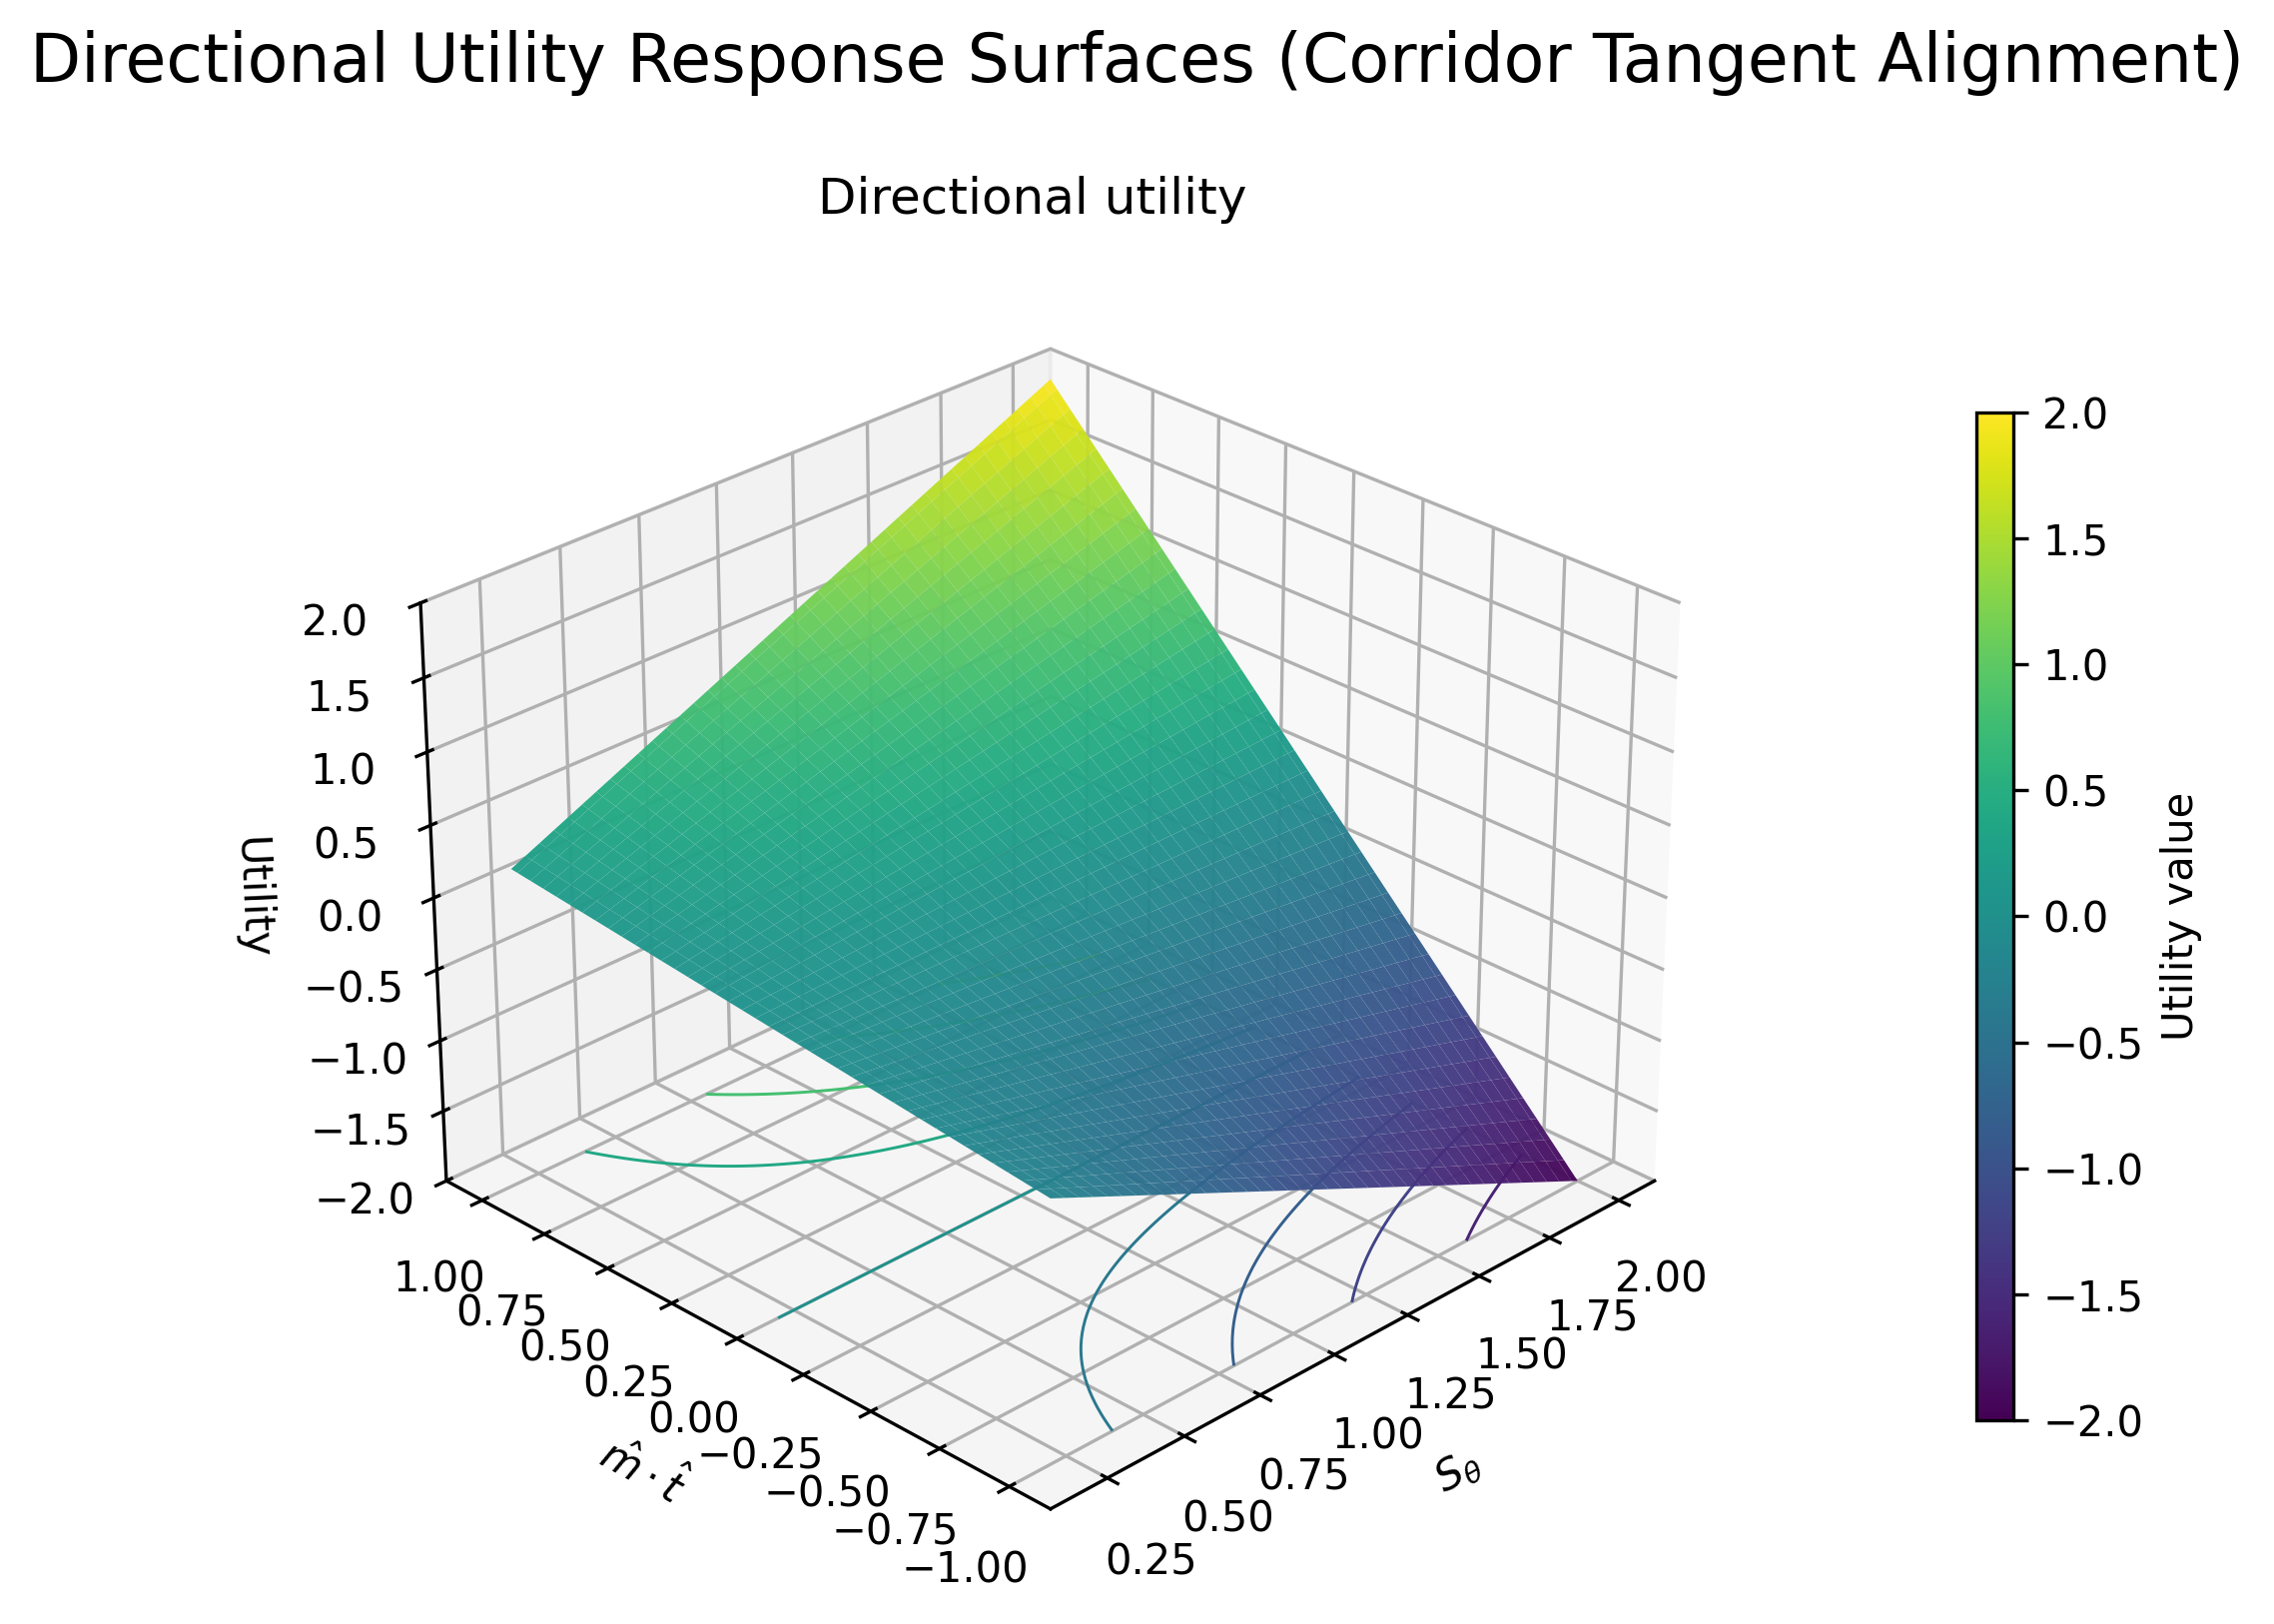
\includegraphics[width=0.45\textwidth]{Appendix/directional_utility_surface_slices.png}
    \caption{Directional utility \(U_{\mathrm{dir}}\) versus corridor alignment \(\hat{m}\cdot\hat{t}\) and directional sensitivity \(S_{\theta}\).}
    \label{fig41}
\end{figure}

\subsection*{Speed Incentive}
Speed utility rewards candidate bicycle-rollout speeds close to a desired speed. Define the symmetric closeness ratio
\begin{equation}
\rho
=
\frac{\min(v_{\mathrm{cand}},v_{\mathrm{des}})}{\max(v_{\mathrm{cand}},v_{\mathrm{des}})}
\in(0,1],
\end{equation}
and
\begin{equation}
U_{\mathrm{speed}}
=
S_{v}
\frac{\rho}{1+\rho^{(\xi_i-1)/2}}.
\end{equation}
The corresponding partial derivatives are
\begin{align}
\frac{\partial U_{\mathrm{speed}}}{\partial S_v}
&=
\frac{\rho}{1+\rho^{(\xi_i-1)/2}}, \\
\frac{\partial U_{\mathrm{speed}}}{\partial \xi_i}
&=
-
\frac{S_v\,\rho^{(\xi_i+1)/2}\ln\rho}{2\big(1+\rho^{(\xi_i-1)/2}\big)^2}.
\end{align}
Utility attains its maximum at \(v_{\mathrm{cand}}=v_{\mathrm{des}}\) (\(\rho=1\)). Overspeeding and underspeeding are penalized symmetrically. Larger \(\xi_i\) sharpens the drop in utility away from the desired speed, making the agent more sensitive to speed mismatch.

\begin{figure*}[!t]
    \centering
    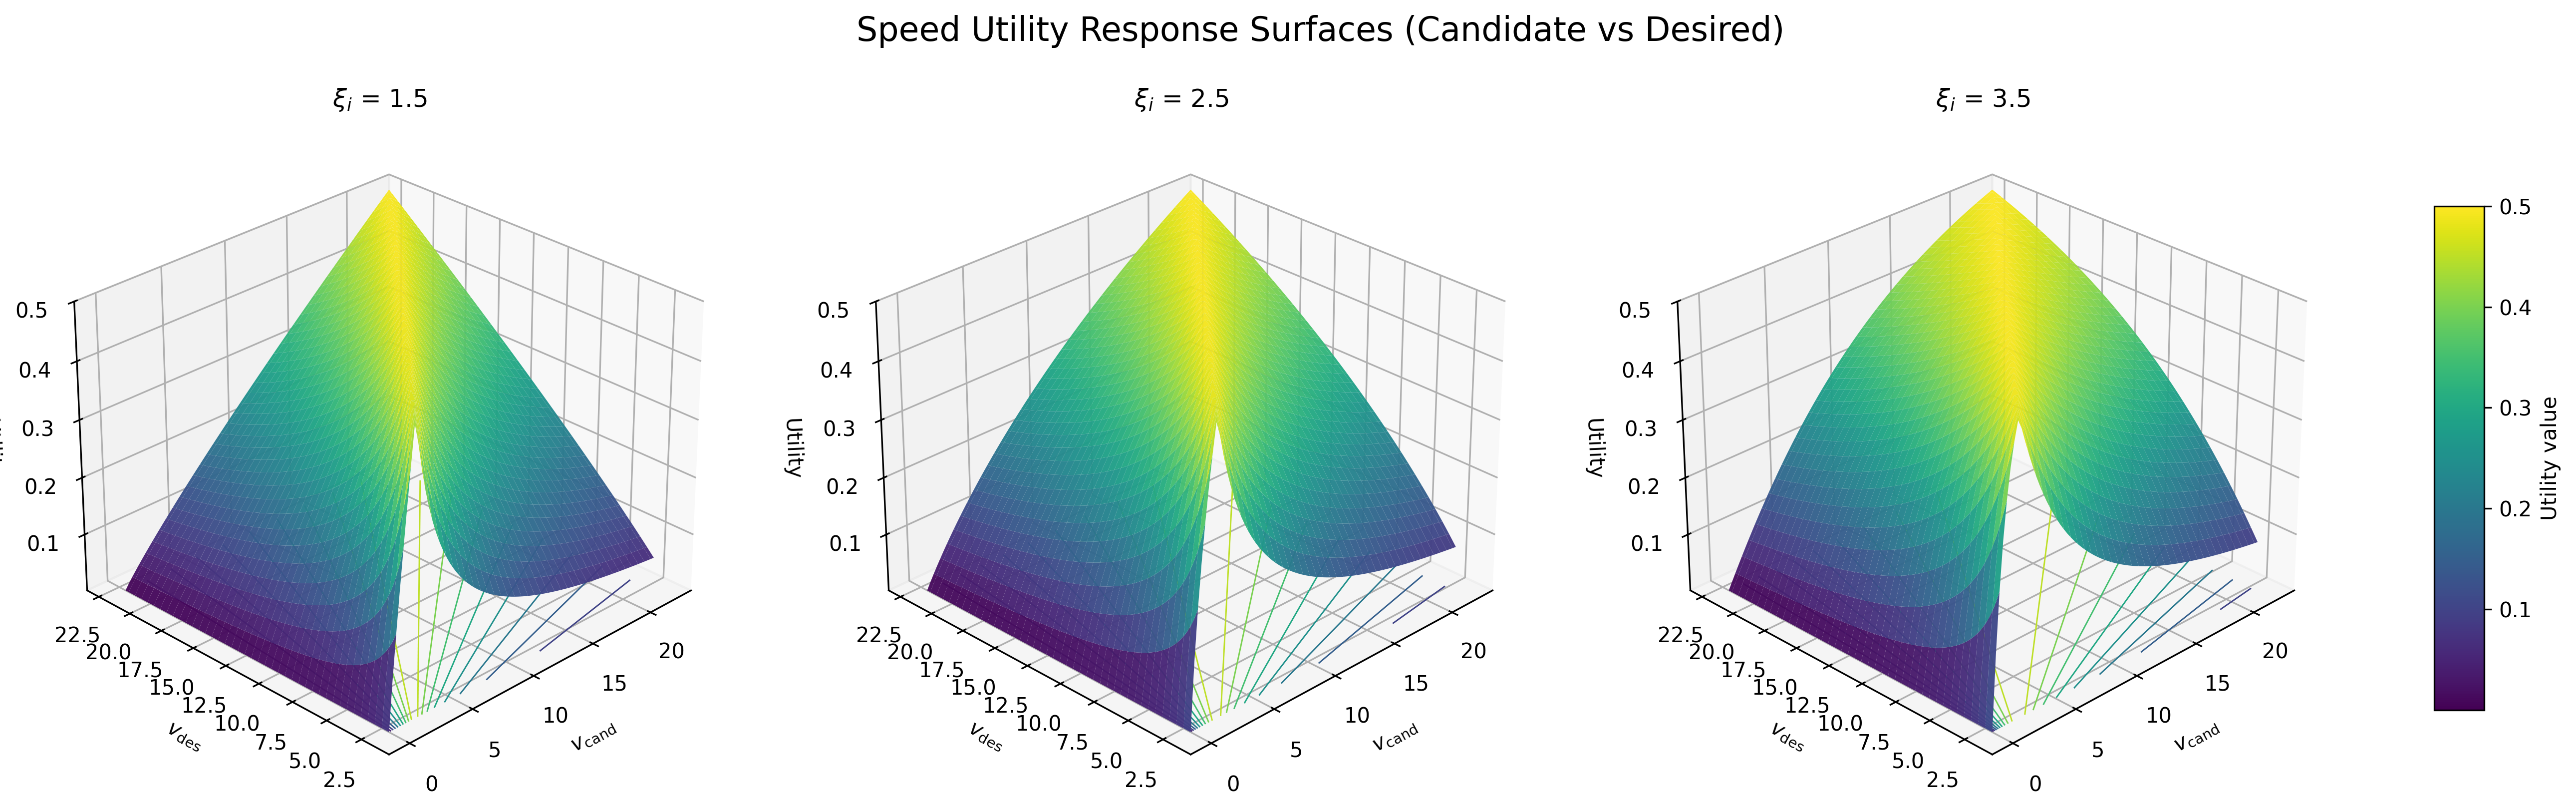
\includegraphics[width=1.0\textwidth]{Appendix/speed_utility_surface_slices.png}
    \caption{Speed utility \(U_{\mathrm{speed}}\) versus candidate speed \(v_{\mathrm{cand}}\) and desired speed \(v_{\mathrm{des}}\) (with \(\xi_i\) slices).}
    \label{fig42}
\end{figure*}

\subsection*{Proximity Incentive}
Proximity utility encourages progress toward a local corridor reference expressed in Frenet coordinates. The effective distance is
\begin{equation}
d_{\mathrm{eff}}
=
w_x|\Delta s|
+
w_y|\Delta n|,
\end{equation}
and
\begin{equation}
U_{\mathrm{dist}}
=
\frac{S_d}{1+(d_{\mathrm{eff}}/H_p)^{\gamma}},
\quad
H_p=\max(\kappa v_i,H_{\min}).
\end{equation}
The primary sensitivities are
\begin{align}
\frac{\partial U_{\mathrm{dist}}}{\partial S_d}
&=
\frac{1}{1+(d_{\mathrm{eff}}/H_p)^{\gamma}}, \\
\frac{\partial U_{\mathrm{dist}}}{\partial \gamma}
&=
-
S_d
\frac{(d_{\mathrm{eff}}/H_p)^{\gamma}\ln(d_{\mathrm{eff}}/H_p)}{\big(1+(d_{\mathrm{eff}}/H_p)^{\gamma}\big)^2}, \\
\frac{\partial U_{\mathrm{dist}}}{\partial d_{\mathrm{eff}}}
&=
-
S_d
\frac{\gamma (d_{\mathrm{eff}}/H_p)^{\gamma}}{d_{\mathrm{eff}}\big(1+(d_{\mathrm{eff}}/H_p)^{\gamma}\big)^2}, \\
\frac{\partial U_{\mathrm{dist}}}{\partial H_p}
&=
S_d
\frac{\gamma (d_{\mathrm{eff}}/H_p)^{\gamma}}{H_p\big(1+(d_{\mathrm{eff}}/H_p)^{\gamma}\big)^2}.
\end{align}
Here \(S_d\) scales importance, \(\gamma\) controls how quickly the reward decays outside the horizon, \(w_x\) and \(w_y\) weight longitudinal versus lateral Frenet error, and \(H_p\) softens normalized distance as speed increases.

\begin{figure*}[!t]
    \centering
    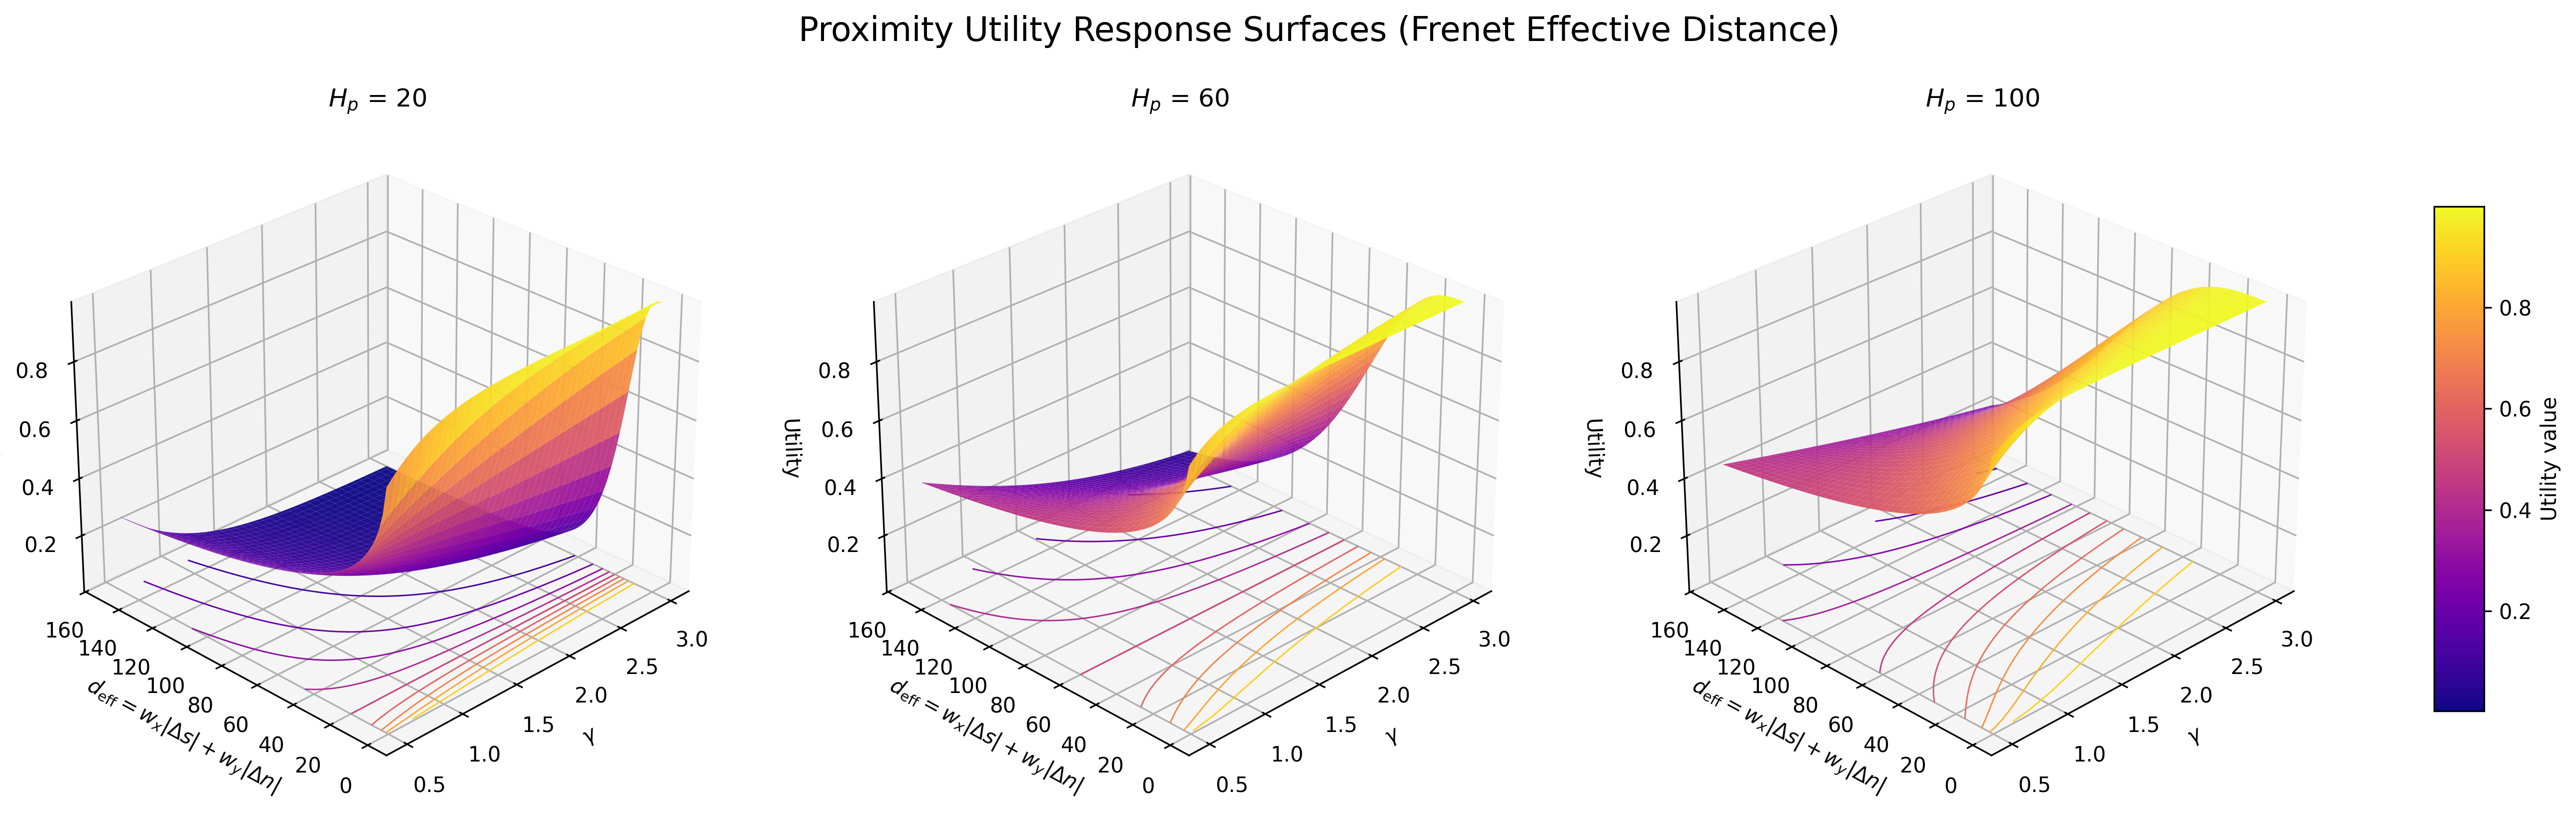
\includegraphics[width=1.0\textwidth]{Appendix/proximity_utility_surface_slices.png}
    \caption{Proximity utility \(U_{\mathrm{dist}}\) versus interaction exponent \(\gamma\), effective Frenet distance \(d_{\mathrm{eff}}\), and perception horizon \(H_p\).}
    \label{fig43}
\end{figure*}

\subsection*{Collision-Risk Penalty}
The primary partial derivatives for the collision-risk penalty in Eq.~\eqref{eq:utility} are
\begin{align}
U_{\mathrm{col}}
&=
w_c \min\!\Bigl(\sum_{j} P_{j,i'},\,1\Bigr), \\
\frac{\partial U_{\mathrm{col}}}{\partial w_c}
&=
\min\!\Bigl(\sum_{j} P_{j,i'},\,1\Bigr),
\end{align}
with $P_{j,i'}=\exp(-\tfrac12[(g_{\parallel}/\sigma_{\parallel})^{2}+(g_{\perp}/\sigma_{\perp})^{2}])$ on OBB surface gaps. Increasing $w_c$ makes the utility more sensitive to predicted overlap and therefore promotes more risk-averse behavior. Small $(\sigma_{\parallel},\sigma_{\perp})$ sharpen the risk field around the footprints; large scales broaden it.

Fig.~\ref{fig44} shows this kernel at $\theta_{\mathrm{rob}}$: unit presence on overlapping $L\times W$ boxes, then anisotropic decay on the surface gaps $(g_{\parallel},g_{\perp})$.

\begin{figure*}[!t]
    \centering
    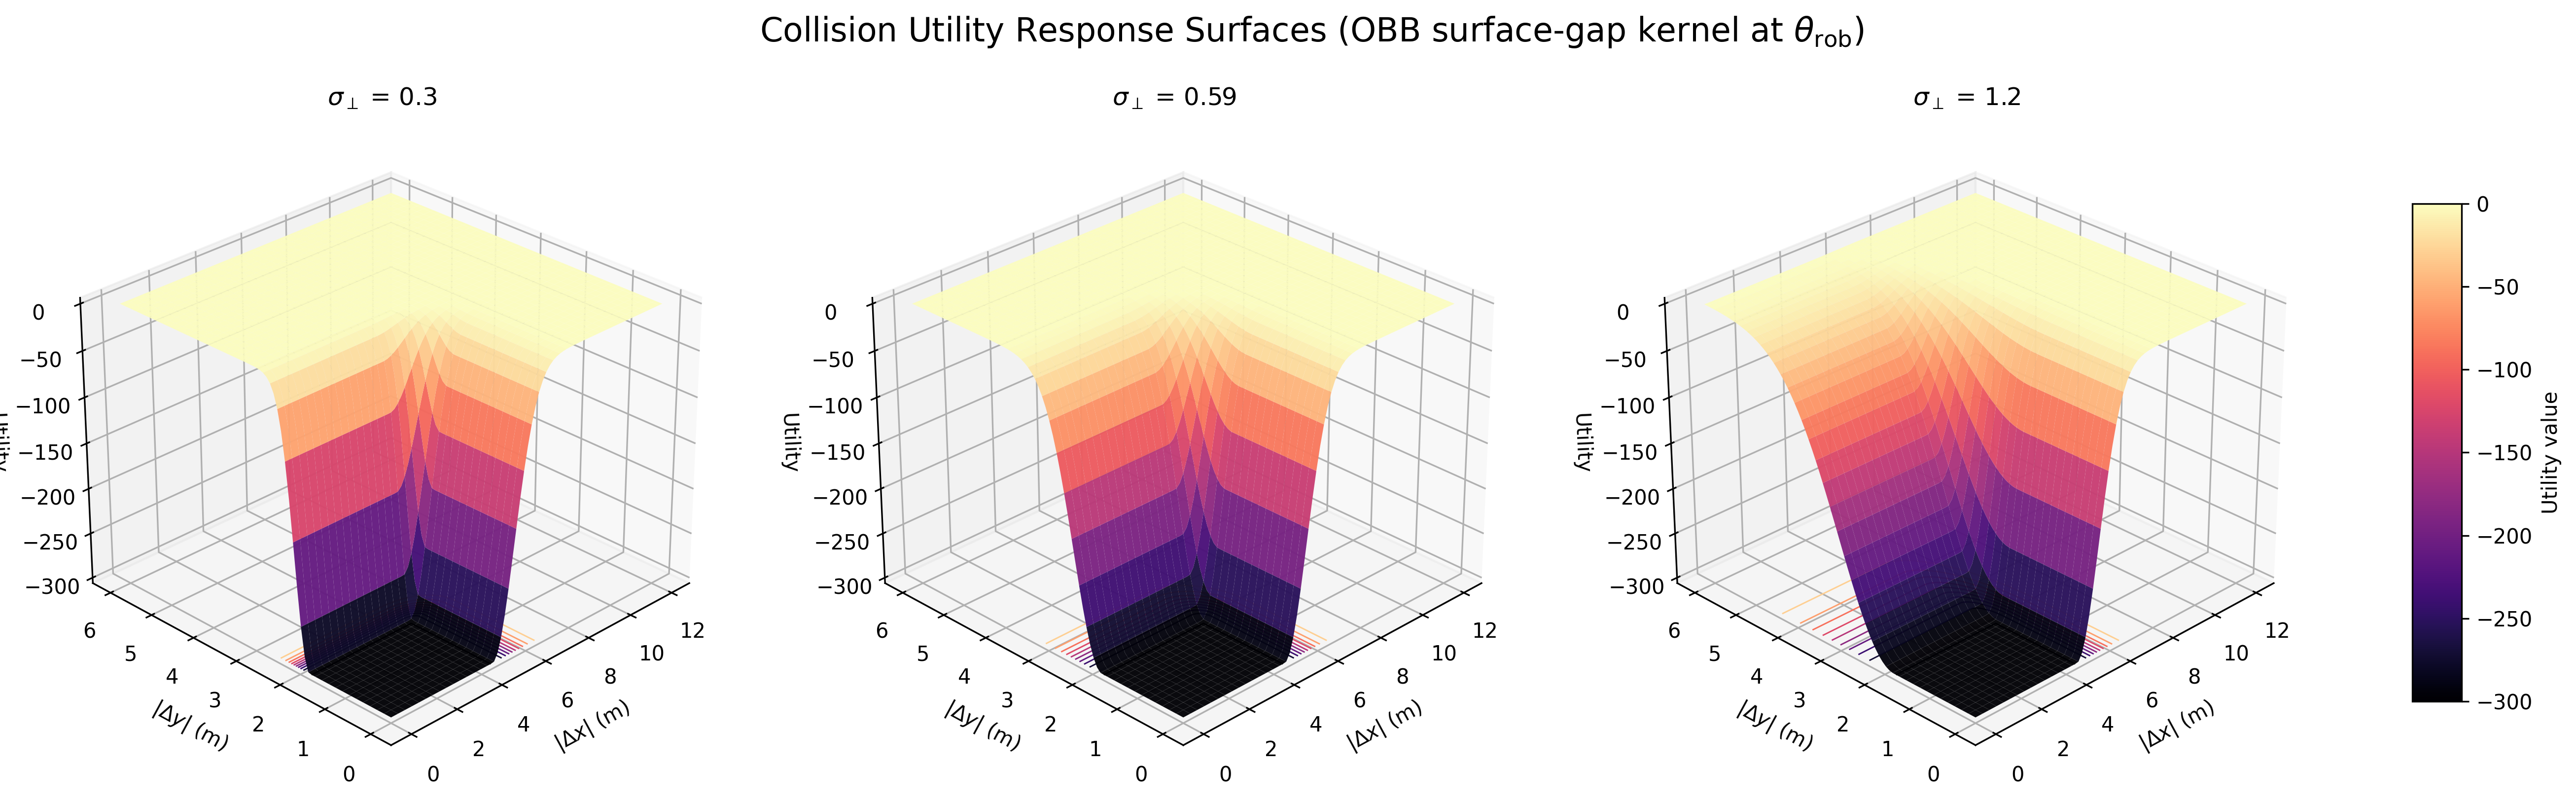
\includegraphics[width=1.0\textwidth]{Appendix/collision_utility_surface_slices.png}
    \caption{Collision utility $U_{\mathrm{col}}=-w_c P$ versus body-frame centre separations $|\Delta x|,|\Delta y|$ at $w_c=300$, $\sigma_{\parallel}=0.89\,\mathrm{m}$, $L\times W=4.5\times 1.8\,\mathrm{m}$. Panels vary $\sigma_{\perp}$; the flat well is the overlapping-footprint plateau.}
    \label{fig44}
\end{figure*}

\subsection*{Path Adherence}
The path-adherence term and its derivatives are
\begin{align}
U_{\mathrm{path}}
&=
w_{\ell}\big(1-e^{-\beta\ell_i^2}\big), \\
\frac{\partial U_{\mathrm{path}}}{\partial w_{\ell}}
&=
1-e^{-\beta\ell_i^2}, \\
\frac{\partial U_{\mathrm{path}}}{\partial \beta}
&=
w_{\ell}\ell_i^2 e^{-\beta\ell_i^2}, \\
\frac{\partial U_{\mathrm{path}}}{\partial \ell_i}
&=
2\,w_{\ell}\beta\ell_i e^{-\beta\ell_i^2}.
\end{align}
Here \(\ell_i\) is a non-negative corridor-boundary residual, \(w_{\ell}\) scales the penalty magnitude, and \(\beta\) controls how quickly the penalty saturates near the boundary. Larger \(w_{\ell}\) enforces stricter corridor adherence but may conflict with collision avoidance or progress when set excessively high.

\begin{figure*}[!t]
    \centering
    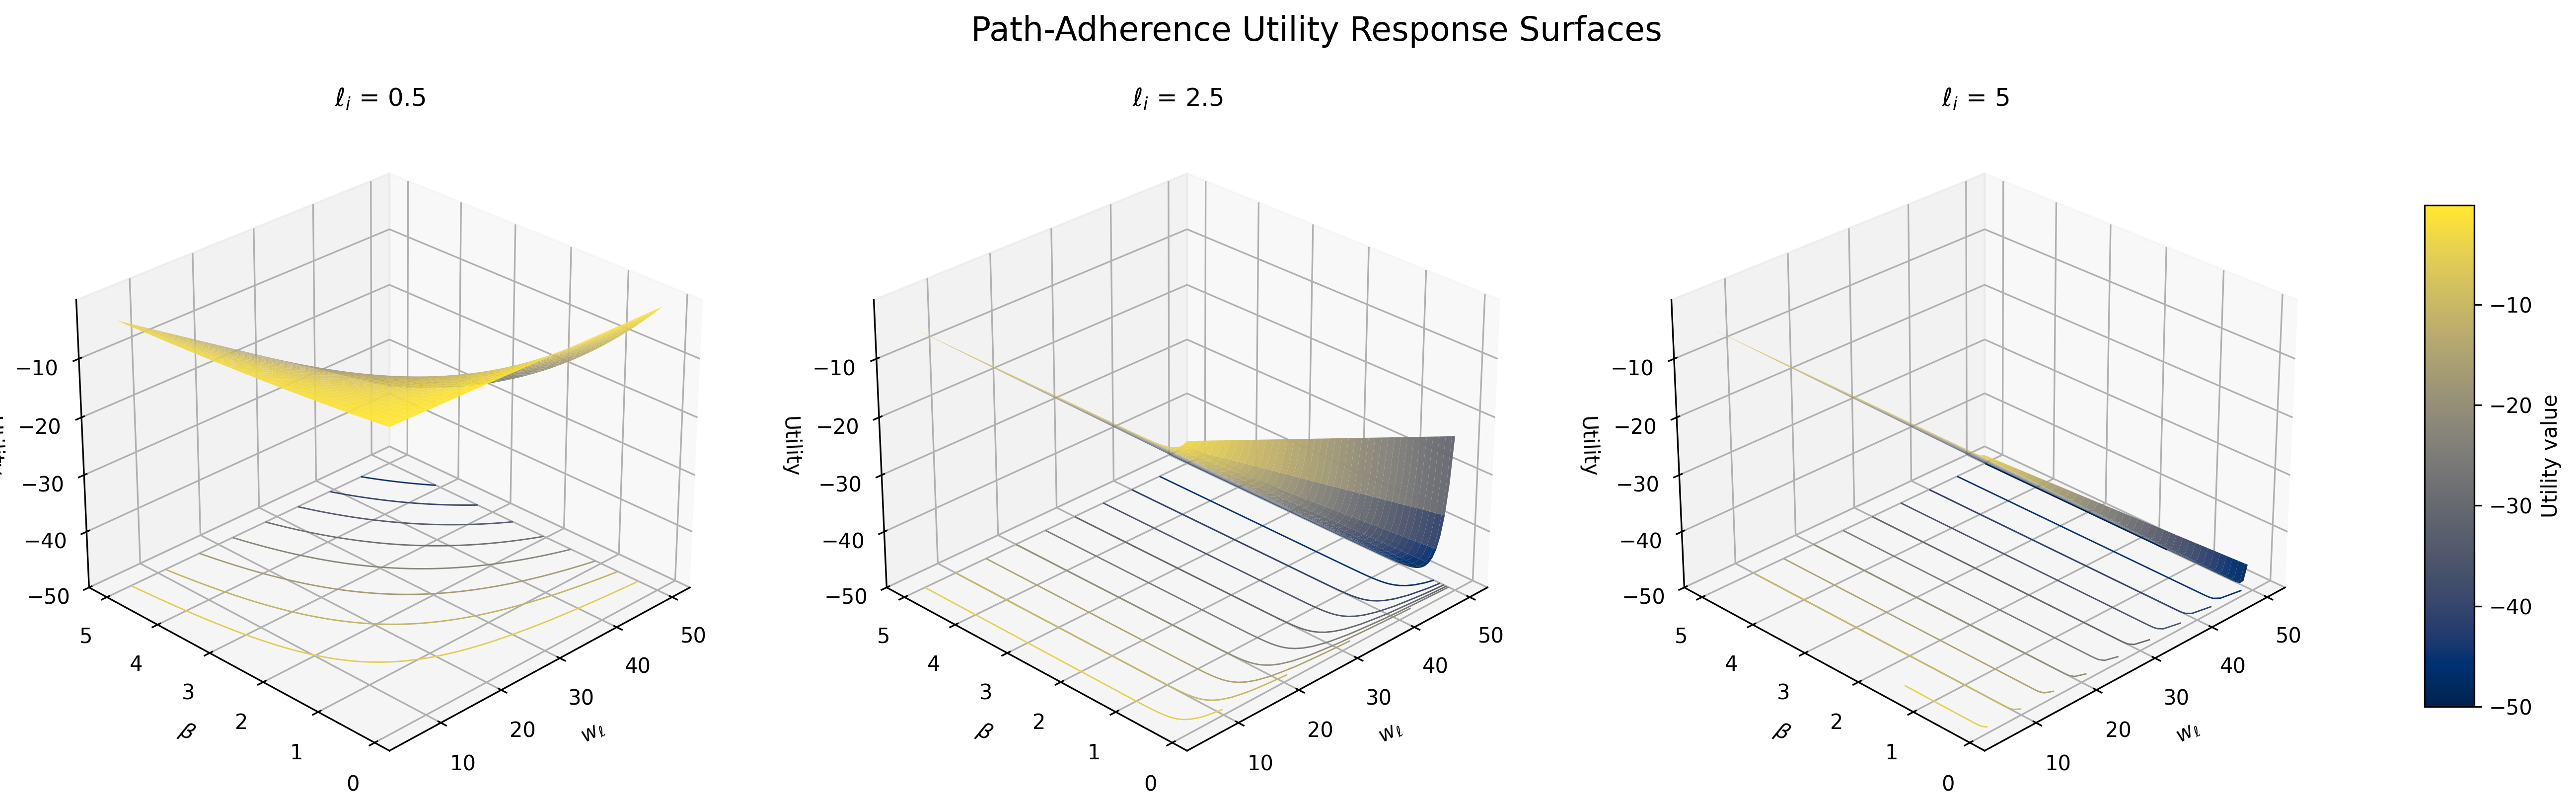
\includegraphics[width=1.0\textwidth]{Appendix/path_adherence_utility_surface_slices.png}
    \caption{Path-adherence utility \(U_{\mathrm{path}}\) versus path-deviation coefficient \(\beta\) and lateral deviation \(\ell_i\).}
    \label{fig45}
\end{figure*}

\section{Global Sensitivity Analysis}

The Sobol study in this appendix is a \emph{pre-recalibration}, ten-parameter scan: it omits $(\sigma_{\parallel},\sigma_{\perp})$ and uses the ad-hoc boxes in Table~\ref{tab:gsa_param_ranges_report}, which do \emph{not} contain the working point $\theta_{\mathrm{rob}}$ (e.g., $S_{\theta}=4.13$ and $w_{c}=300$ lie outside $[0.2,1]$ and $[0.1,20]$). The indices below therefore describe that older box, not the calibrated operating region. As noted in the limitations, a GSA aligned with the top-cloud percentiles would be required before treating these rankings as structural.

Global Sensitivity Analysis (GSA) quantifies how uncertainty in the model output is attributed to uncertainty in the model parameters. Unlike local sensitivity analysis, which perturbs one parameter around a nominal value, GSA evaluates the entire parameter space and captures both direct parameter effects and higher-order interactions.

The proposed framework represents traffic agents moving in continuous two-dimensional space. At each simulation step, every agent generates feasible acceleration and steering candidates using the kinematic bicycle model and selects the candidate that maximizes the utility function defined in Equation~\ref{eq:utility}. The utility consists of corridor directional preference, speed incentive, Frenet-distance proximity incentive, collision-risk penalty, and path-adherence penalty.

The model performance is evaluated using the following simulation-level objective:
\begin{equation}
\label{eq:performance_metric_Y}
Y
=
\sum_{k\in\mathcal{A}}
d_k^{\mathrm{final}}
+
N_{\mathrm{coll}}\,C_{\mathrm{penalty}},
\end{equation}
where \(d_k^{\mathrm{final}}\) denotes the final Euclidean distance between agent \(k\) and its destination, \(N_{\mathrm{coll}}\) is the total number of collision events during the simulation, and \(C_{\mathrm{penalty}}\) is a fixed collision penalty. Lower values of \(Y\) correspond to better overall system performance.

The sensitivity analysis is performed using the variance-based Sobol method \cite{sobol1990sensitivity,saltelli2010variance}. Let the model output be

\[
Y=f(X_1,X_2,\ldots,X_D),
\]

where \(X_j\) represents independent model parameters. The output variance is decomposed as

\begin{equation}
\label{eq:variance_decomposition}
\mathrm{Var}(Y)
=
\sum_{j=1}^{D}V_j
+
\sum_{1\le j<k\le D}V_{jk}
+\cdots+
V_{12\ldots D}.
\end{equation}

The first-order Sobol index is

\begin{equation}
\label{eq:S1_def}
S_j
=
\frac{V_j}{\mathrm{Var}(Y)},
\end{equation}

while the total-order Sobol index is

\begin{equation}
\label{eq:ST_def}
S_{T_j}
=
1-
\frac{
\mathrm{Var}_{\mathbf{X}_{\sim j}}
\!\left(
\mathbb{E}_{X_j}
\left[
Y\mid
\mathbf{X}_{\sim j}
\right]
\right)
}
{\mathrm{Var}(Y)}.
\end{equation}

The first-order index quantifies the direct contribution of parameter \(X_j\) to the output variance, whereas the total-order index measures its overall contribution, including all interaction effects.

Sampling is performed using Sobol quasi-random sequences generated with the \texttt{SALib} library. A base sample size of \(N=1024\) is used for the ten-dimensional parameter space, resulting in

\[
N_{\mathrm{eval}}
=
N(D+2)
=
1024(10+2)
=
12288
\]

simulation evaluations.

Table~\ref{tab:gsa_param_ranges_report} summarizes the parameter ranges considered during the sensitivity analysis.

\begin{table}[h]
\centering
\caption{Model parameters and predefined ranges used in the Sobol sensitivity analysis (pre-recalibration box; does not contain $\theta_{\mathrm{rob}}$).}
\label{tab:gsa_param_ranges_report}
\begin{tabular}{llr}
\hline
Parameter & Description & Range\\
\hline
\(S_{\theta}\) & Corridor directional weight & \([0.2,1.0]\)\\
\(S_v\) & Speed-incentive weight & \([0.2,1.0]\)\\
\(\xi_i\) & Speed-mismatch steepness & \([1.5,3.5]\)\\
\(S_d\) & Proximity-incentive weight & \([0.2,1.0]\)\\
\(\gamma\) & Proximity decay steepness & \([0.5,3.0]\)\\
\(w_x\) & Longitudinal Frenet weight & \([0.5,5.0]\)\\
\(w_y\) & Lateral Frenet weight & \([0.5,5.0]\)\\
\(w_c\) & Collision-risk penalty weight & \([0.1,20.0]\)\\
\(w_{\ell}\) & Path-adherence penalty weight & \([5.0,50.0]\)\\
\(\beta\) & Path-adherence saturation rate & \([0.1,5.0]\)\\
\hline
\end{tabular}
\end{table}

The proximity incentive employs the Frenet effective distance

\begin{equation}
d_{\mathrm{eff}}
=
w_x|\Delta s|
+
w_y|\Delta n|,
\end{equation}

while the perception horizon is computed as

\begin{equation}
H_p
=
\max(\kappa v_i,H_{\min}).
\end{equation}

The speed incentive uses the normalized speed ratio

\begin{equation}
\rho
=
\frac{\min(v_{\mathrm{cand}},v_{\mathrm{des}})}
{\max(v_{\mathrm{cand}},v_{\mathrm{des}})}.
\end{equation}

Collision risk follows the vehicle-footprint kernel in the main methodology (OBB surface gaps in the ego body frame, weighted by \(w_c\)). The Sobol box below does not vary \((\sigma_{\parallel},\sigma_{\perp})\).

\subsection{Sensitivity Analysis Results}

Table~\ref{tab:sobol_results} summarizes the estimated first-order and total-order Sobol indices for all utility parameters.

\begin{table}[h]
\centering
\caption{Sobol sensitivity indices and associated confidence intervals.}
\label{tab:sobol_results}
\begin{tabular}{lcccc}
\hline
Parameter & \(S_1\) & \(S_{1,\mathrm{conf}}\) & \(S_T\) & \(S_{T,\mathrm{conf}}\)\\
\hline
\(S_{\theta}\) & 0.128 & 0.025 & 0.353 & 0.029\\
\(S_v\)        & 0.287 & 0.031 & 0.598 & 0.041\\
\(\xi_i\)      & -0.001 & 0.011 & 0.060 & 0.012\\
\(S_d\)        & 0.005 & 0.010 & 0.035 & 0.006\\
\(\gamma\)     & 0.003 & 0.006 & 0.021 & 0.005\\
\(w_x\)        & 0.033 & 0.016 & 0.109 & 0.013\\
\(w_y\)        & 0.017 & 0.011 & 0.065 & 0.011\\
\(w_c\)        & 0.000 & 0.000 & 0.000 & 0.000\\
\(w_{\ell}\)   & 0.043 & 0.022 & 0.247 & 0.027\\
\(\beta\)      & 0.119 & 0.033 & 0.390 & 0.029\\
\hline
\end{tabular}
\end{table}

The sensitivity analysis demonstrates that the speed-incentive weight \(S_v\) is the dominant model parameter, exhibiting the largest first-order and total-order sensitivity indices. The path-adherence saturation parameter \(\beta\) and the corridor directional weight \(S_{\theta}\) are the next most influential parameters, followed by the path-adherence penalty weight \(w_{\ell}\). These four parameters account for the majority of the variance in the simulation-level performance metric.

For the dominant parameters, the total-order indices are substantially larger than the corresponding first-order indices, indicating that their influence arises not only from direct effects but also through interactions with other utility terms. In contrast, the proximity-related parameters (\(S_d\), \(\gamma\), \(w_x\), and \(w_y\)) exhibit comparatively small sensitivities, suggesting that variations within the investigated ranges have only a limited impact on overall model performance.

The collision-risk penalty weight \(w_c\) exhibits negligible first-order and total-order sensitivity \emph{inside this box}. That is expected: the sampled range \([0.1,20]\) never reaches the calibrated operating value \(w_c\approx 300\), and sparse simulated collisions contribute little to \(Y\). It should not be read as evidence that collision aversion is unimportant at \(\theta_{\mathrm{rob}}\).

Overall, within the investigated (off-regime) ranges the GSA ranks \(S_v\), \(\beta\), \(S_{\theta}\), and \(w_{\ell}\) as the most influential coordinates. Those rankings are not a substitute for identifiability diagnostics on the calibrated cloud (Fig.~\ref{fig:calibration_identifiability}).


\section{Datasets}
\label{app:datasets}

The main text evaluates residual MARL on a single weak-lane freeway corridor. The utility prior itself, however, is geometry-aware rather than lane-ID-based, so the same five-term family~\eqref{eq:utility} can be instantiated on qualitatively different roadways if the directional, proximity, and path terms are evaluated in a site-appropriate spatial frame. This appendix documents three naturalistic environments used for that purpose (Fig.~\ref{fig:datasets_sites}): the Lebanon Highway freeway that supports the main residual-learning experiments, a compact multi-arm roundabout also collected in Jounieh, and the TGSIM Foggy Bottom urban street network in Washington, DC. Residual MARL, planner comparatives, and the dense-stress protocol are \emph{not} repeated on the two urban sites; those recordings are used only to test whether a calibrated utility prior remains meaningful when the corridor assumption is replaced by a destination-plus-curb encoding.

\begin{figure}[t]
\centering
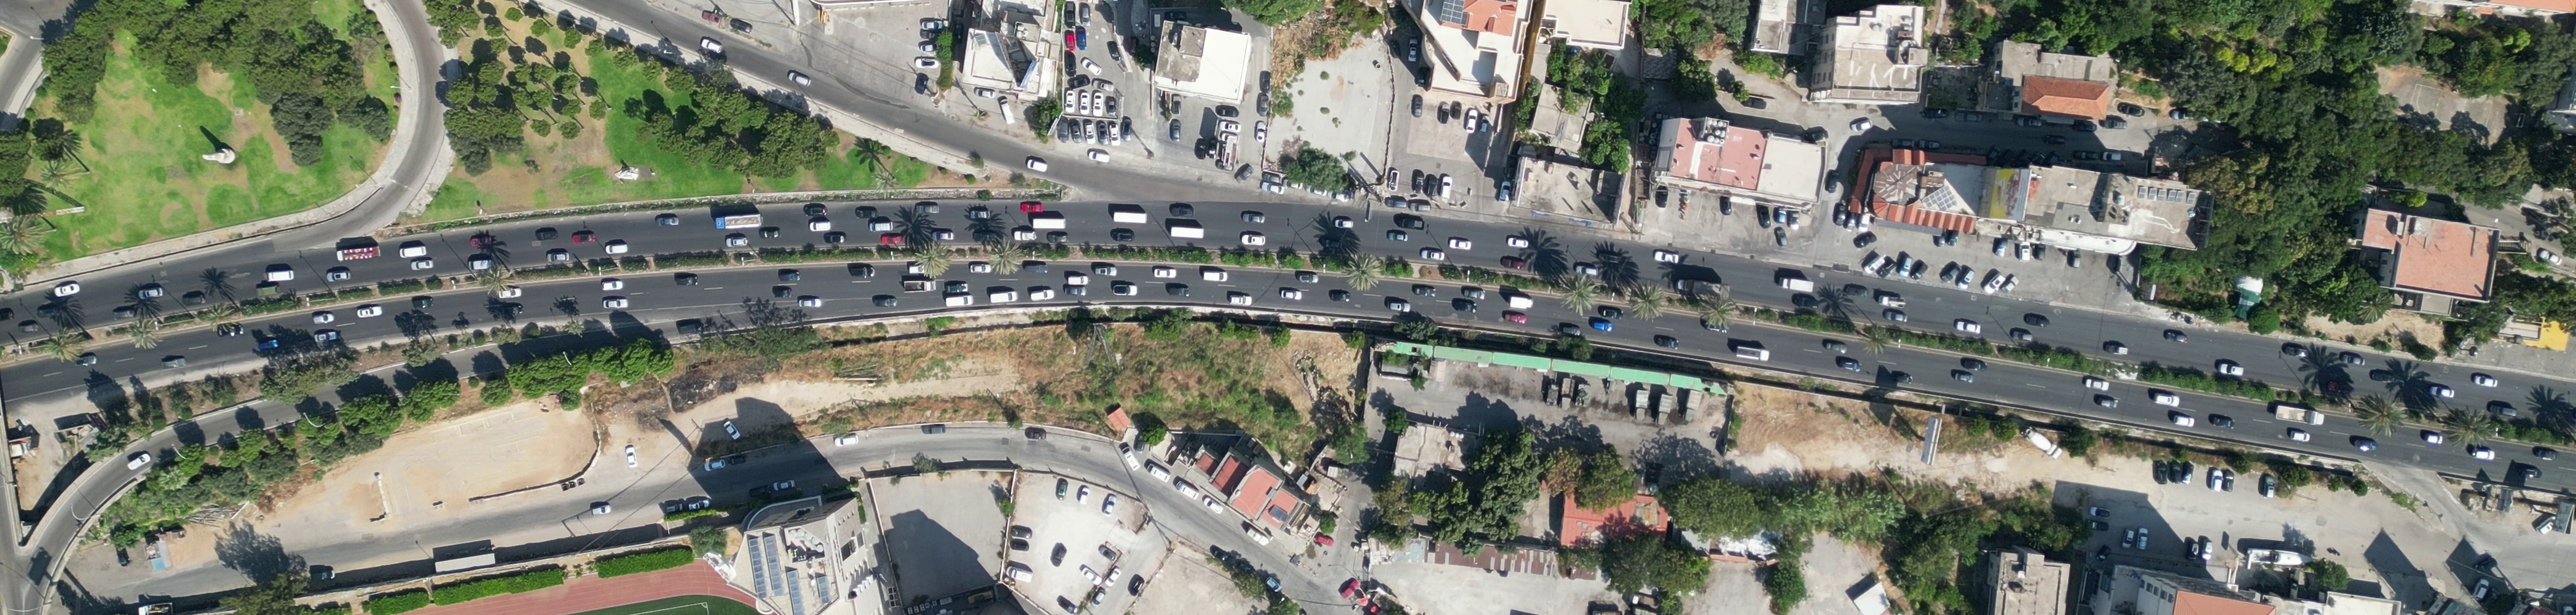
\includegraphics[width=0.92\linewidth]{Pics/Frame.jpg}
\caption{Aerial frame of the Jounieh study area (weak-lane, heterogeneous traffic) ~\cite{khoueiry2025universal}.}
\label{fig:app_freeway_frame}
\end{figure}

\begin{figure}[t]
\centering
\includegraphics[width=0.92\linewidth]{Pics/JouFrame.jpg}
\caption{Aerial frame of the Jounieh study area.}
\label{fig:app_freeway_frame}
\end{figure}

\begin{figure}[t]
\centering
\includegraphics[width=0.92\linewidth]{Pics/TGSIMFrame.jpg}
\caption{Aerial frame of the TGSIM Foggy Bottom study area}
\label{fig:app_freeway_frame}
\end{figure}

\begin{figure*}[t]
\centering
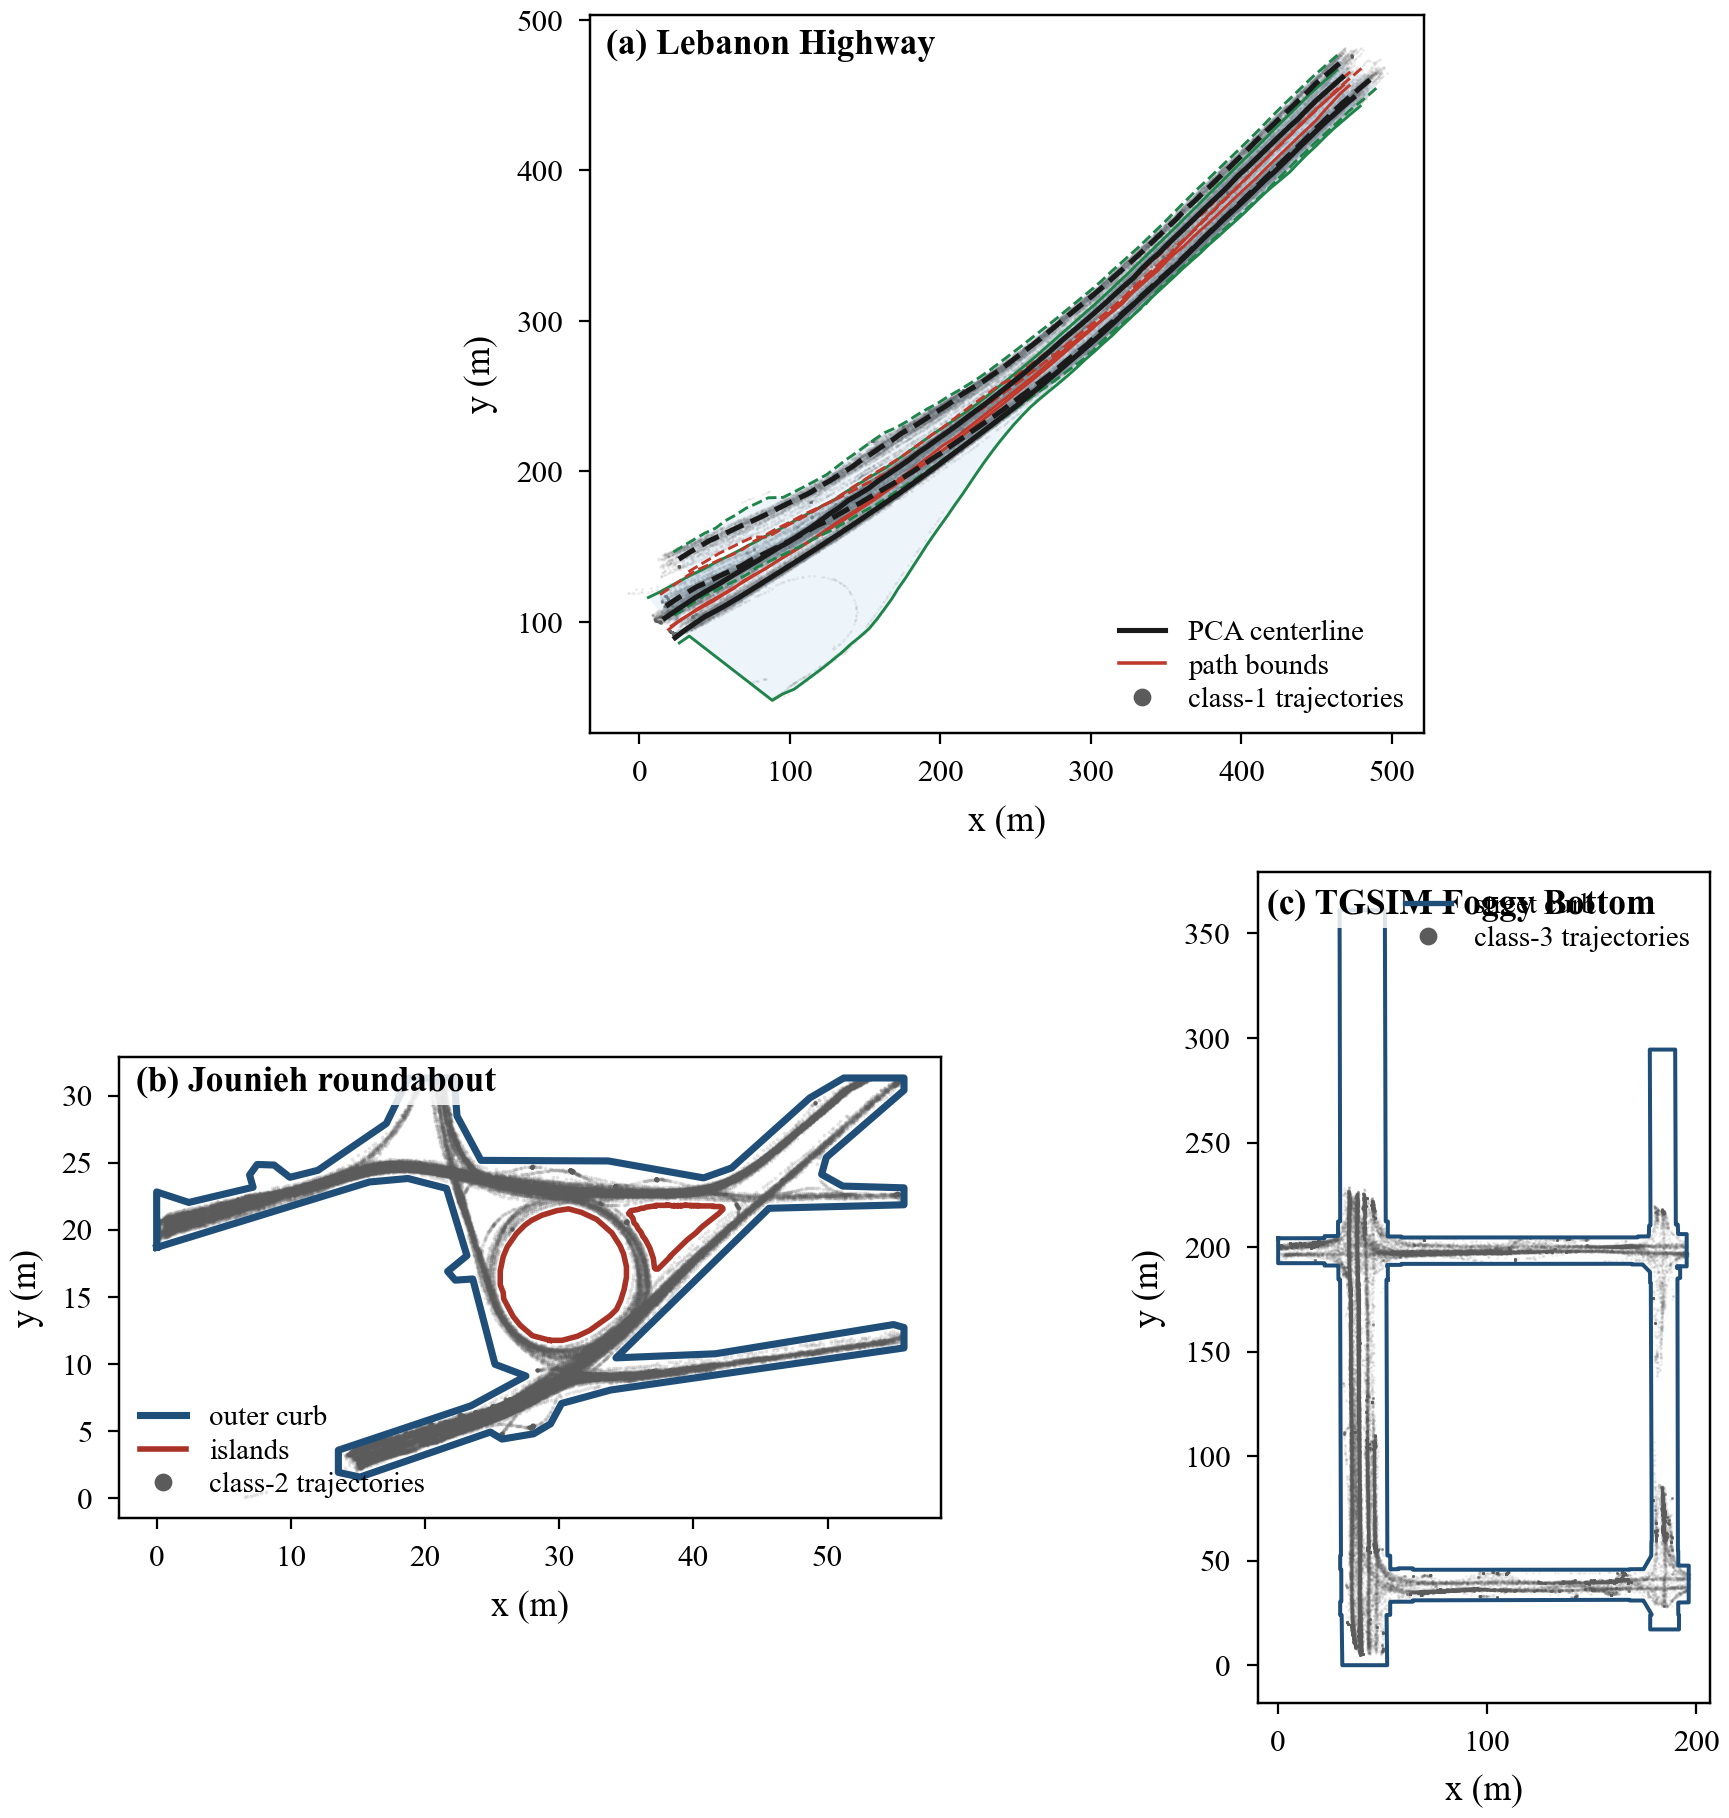
\includegraphics[width=\textwidth]{Appendix/fig_datasets_sites.png}
\caption{Reconstructed geometry and ego-class trajectories for the three calibration environments. (a)~Lebanon Highway: per-stream PCA centerlines (black) and path-adherence bounds (red/green) over class-1 passenger-vehicle points. Solid and dashed tubes correspond to the two recordings. (b)~Jounieh roundabout: one outer curb (blue) and interior islands (red) shared by all class-2 tracks. (c)~TGSIM Foggy Bottom: union street curb (blue) over class-3 passenger-car points.}
\label{fig:datasets_sites}
\end{figure*}

Table~\ref{tab:app_dataset_summary} summarizes the calibration-ready samples. All three sources are subsampled to $\Delta t\approx 0.1$\,s. For the two urban sites we drop any track that is shorter than $10$\,s, whose $85$th-percentile speed is below $1$\,m/s, or whose travelled path is shorter than $8$\,m, so that parked and fragmentary objects never enter the ego pool or the neighbor set. The freeway calibration uses passenger vehicles (class~$1$) with valid kinematic transitions, as in Section~\ref{sec:calibration_methodology}. Urban calibrations use the dominant moving class at each site (class~$2$ at the roundabout; class~$3$ passenger cars at Foggy Bottom). Neighbor footprints default to $4.5\,\mathrm{m}\times 1.8\,\mathrm{m}$ unless a site file supplies length/width.

\begin{table*}[t]
\centering
\caption{Calibration-ready trajectory samples used in this appendix. Counts refer to the ego class listed in the second column. Durations and speeds are medians over ego tracks.}
\label{tab:app_dataset_summary}
\small
\begin{tabular}{lccccccc}
\toprule
Site & Tracks & Med.\ duration (s) & Med.\ speed (m/s) & $v_{85}$ / $v_{99}$ (m/s) & Extent (m) & Geometry \\
\midrule
Lebanon Highway      & $368$  & $57.8$ & $8.15$ & $11.6$ / $16.3$ & $505\times 433$ & PCA tubes (2 rec.\ $\times$ 2 streams) \\
Jounieh roundabout   & $479$  & $24.4$ & $1.88$ & $2.70$ / $3.89$ & $56\times 31$   & outer curb $+$ 2 islands \\
TGSIM Foggy Bottom   & $2773$ & $25.2$ & $1.61$ & $9.59$ / $16.3$ & $197\times 224$ & union street curb \\
\bottomrule
\end{tabular}
\end{table*}

\subsection{Lebanon Highway}
The primary study site is a multilane urban freeway in Jounieh, Lebanon, recorded by a near-stationary drone under weak lane discipline (Fig.~\ref{fig:app_freeway_frame}). Extraction and operational details are given by Khoueiry et al.~\cite{khoueiry2025universal}. Two complementary recordings (\texttt{run\_id}$\in\{1,2\}$) cover the same curved corridor in opposite observational conditions; each recording is reconstructed into two Kalman-filter movement streams (\texttt{lane\_kf}$\in\{1,2\}$). Rather than relying on painted lane IDs---which are only weakly respected---the spatial reference for utility is a data-driven PCA tube per (\texttt{run\_id}, \texttt{lane\_kf}): a centerline for Frenet/direction terms and lower/upper bounds for $U_{\mathrm{path}}$ (Fig.~\ref{fig:datasets_sites}a). Class-$1$ passenger trajectories ($190{,}767$ valid kinematic transitions from $368$ tracks; median speed $8.15$\,m/s) form the ego pool for the main-text calibration. This is the only environment on which the residual policy is trained and benchmarked.

\subsection{Jounieh Roundabout}
A second Lebanon aerial collection covers a compact multi-arm roundabout (about $56\,\mathrm{m}\times 31\,\mathrm{m}$) rather than a linear corridor. Circulation wraps a large central island and a smaller splitter island; several entries and exits produce crossing and weaving at low speed (median $1.88$\,m/s; $85$th percentile $2.70$\,m/s). A single roadway polygon---outer curb minus the two islands---is used for every vehicle (Fig.~\ref{fig:datasets_sites}b). After the duration/speed/path filter, $479$ class-$2$ tracks remain for calibration. Because there is no unique downstream tangent, directional and proximity terms cannot be taken from a PCA corridor; they are instead destination-based (Section~\ref{app:env_calib}).

\subsection{TGSIM Foggy Bottom}
The third environment is the publicly released TGSIM Foggy Bottom trajectory set~\cite{talebpour2024tgsim,fhwa2024tgsimfb}, collected with overlapping infrastructure cameras around the George Washington University campus in Washington, DC. The reconstructed street graph spans roughly $200\,\mathrm{m}\times 230\,\mathrm{m}$ of signalized and stop-controlled urban links with right-angle turns (Fig.~\ref{fig:datasets_sites}c). Provided lane polygons are unioned into one curb (exterior plus interior holes) that is shared by all IDs. The prepared file retains mixed road-user types after dropping parked/short tracks; we calibrate on class-$3$ passenger cars ($2773$ tracks). Speeds are strongly bimodal: the median ($1.61$\,m/s) reflects queues and turning, while the $85$th/$99$th percentiles ($9.59$ / $16.3$\,m/s) capture unconstrained urban running. As at the roundabout, each track's last observed position is treated as a destination on the roadway polygon.

\section{Environment-based Calibration Results}
\label{app:env_calib}

We reuse the twelve-parameter search, composite objective~\eqref{eq:calibration_objective}, and vehicle-wise train/validation/test split of Section~\ref{sec:calibration_methodology} ($400$ random trials, $3$ restarts, $300$/$100$/$100$ closed-loop windows of horizon $H=8$ steps). Only the spatial encoding of $U_{\mathrm{dir}}$, $U_{\mathrm{dist}}$, and $U_{\mathrm{path}}$ changes with the site; $U_{\mathrm{speed}}$ and $U_{\mathrm{col}}$ keep the same kinematic and probabilistic forms. Collision-kernel scales $(\sigma_{\parallel},\sigma_{\perp})$ remain free parameters.

\paragraph{Corridor versus destination-plus-curb.}
On the freeway, $\hat{t}_{i}$ is the local PCA-tube tangent and $U_{\mathrm{dist}}$ is a Frenet distance to a short-horizon reference along that tube; $U_{\mathrm{path}}$ saturates outside the lower/upper PCA bounds. On the two urban sites this corridor is undefined. Each ego ID is assigned the destination $g_{i}=(x_{i}^{\mathrm{final}},y_{i}^{\mathrm{final}})$ equal to its last observed point (\texttt{utility\_frame=destination}). When a site polygon is supplied, heading incentive and proximity follow the on-road path toward $g_{i}$ on that polygon (around islands and city blocks) rather than the Euclidean chord, and path cost grows with off-road distance. Desired speed remains the track-level desired speed used in the freeway fit; urban kinematic limits follow the site speed distribution. The Jounieh and TGSIM JSON files used here record that polygon path; they are not a second corridor fit.

% Working/test numbers from:
%   calibration/utility_calibration.json            (corridor; freeway)
%   Calibration/utility_calibration_jounieh.json    (destination + site polygon)
%   Calibration/utility_calibration_tgsim.json      (destination + site polygon)

\begin{table*}[t]
\centering
\caption{Environment-based utility calibration. Test $L_{\mathrm{cl}}$ is closed-loop tracking loss on held-out vehicles ($H=8$). Rank is the mean one-step rank of the observed-like candidate during search. Working $(w_{\ell},w_{c})$ come from the validation-selected vector (robust median on the freeway; best-on-validation at the urban sites). All three fits are weakly identified.}
\label{tab:app_env_calib}
\small
\begin{tabular}{llcccccc}
\toprule
Site & Frame & Test $L_{\mathrm{cl}}$ & Val $L_{\mathrm{cl}}$ & Rank & $w_{\ell}$ & $w_{c}$ & Near-opt.\ trials \\
\midrule
Lebanon Highway      & corridor              & $0.565$ & $0.576$ & $5.72$  & $77.6$ & $300$ & $3$ \\
Jounieh roundabout   & destination $+$ curb  & $0.714$ & $0.733$ & $37.9$  & $9.17$ & $71.4$ & $3$ \\
TGSIM Foggy Bottom   & destination $+$ curb  & $0.992$ & $0.965$ & $27.8$  & $68.4$ & $5.92$ & $10^{\dagger}$ \\
\bottomrule
\multicolumn{8}{l}{\footnotesize $^{\dagger}$Top-ten fallback: fewer than three scored trials met the $5\%$ near-optimal cutoff.}
\end{tabular}
\end{table*}

\begin{table}[t]
\centering
\caption{Working utility parameters at each site. Freeway values are the robust median of the near-optimal cloud selected on validation windows; urban values are the best trial on validation windows.}
\label{tab:app_env_params}
\scriptsize
\begin{tabular}{lccc}
\toprule
Parameter & Highway & Jounieh & TGSIM \\
\midrule
$S_{\theta}$ & $4.13$ & $3.88$ & $8.46$ \\
$S_{v}$ & $2.51$ & $3.89$ & $9.68$ \\
$\xi_{i}$ & $4.04$ & $9.83$ & $4.02$ \\
$S_{d}$ & $9.43$ & $8.44$ & $7.76$ \\
$\gamma$ & $0.56$ & $3.63$ & $2.57$ \\
$w_{x}$ & $4.85$ & $5.11$ & $9.49$ \\
$w_{y}$ & $5.83$ & $4.81$ & $2.20$ \\
$w_{c}$ & $300$ & $71.4$ & $5.92$ \\
$w_{\ell}$ & $77.6$ & $9.17$ & $68.4$ \\
$\beta$ & $2.14$ & $6.39$ & $4.59$ \\
$\sigma_{\parallel}$ (m) & $0.89$ & $2.23$ & $0.67$ \\
$\sigma_{\perp}$ (m) & $0.59$ & $1.42$ & $2.46$ \\
\bottomrule
\end{tabular}
\end{table}

\paragraph{Closed-loop scores.}
Held-out tracking is strongest on the freeway (test $L_{\mathrm{cl}}=0.565$), where a unique downstream tangent exists and the PCA tube already concentrates the data. The roundabout remains usable ($0.714$) despite low speeds and circulating geometry. Foggy Bottom is the most demanding ($0.992$): vehicles approach a destination through intersections, queues, and right-angle turns, so an eight-step utility rollout has more ways to miss the observed branch. In all three cases the validation-selected working point generalizes (test is within about $5\%$ of validation), so the gap across sites is geometric rather than an overfit of the search.

\paragraph{One-step ranking and identifiability.}
One-step ranking of the observed-like candidate remains informative on the freeway (mean rank $5.72$) but is close to chance-competitive on both urban sites (Fig.~\ref{fig:app_env_fit}): mean ranks $37.9$ (Jounieh) and $27.8$ (TGSIM) on the discrete acceleration--steering grid, with softmax mass on the target action typically below $0.05$. Soft margins $U_{\mathrm{target}}-\max U_{\mathrm{other}}$ nevertheless concentrate near zero, so the observed action is often a near-maximizer even when it is not rank one. This is consistent with the weakly identified verdict at every site (three near-optimal trials on the freeway and roundabout; top-ten fallback at Foggy Bottom). As in the main text, we therefore treat the working vector as a region of acceptable short-horizon behavior, not a unique structural estimate.

\begin{figure*}[t]
\centering
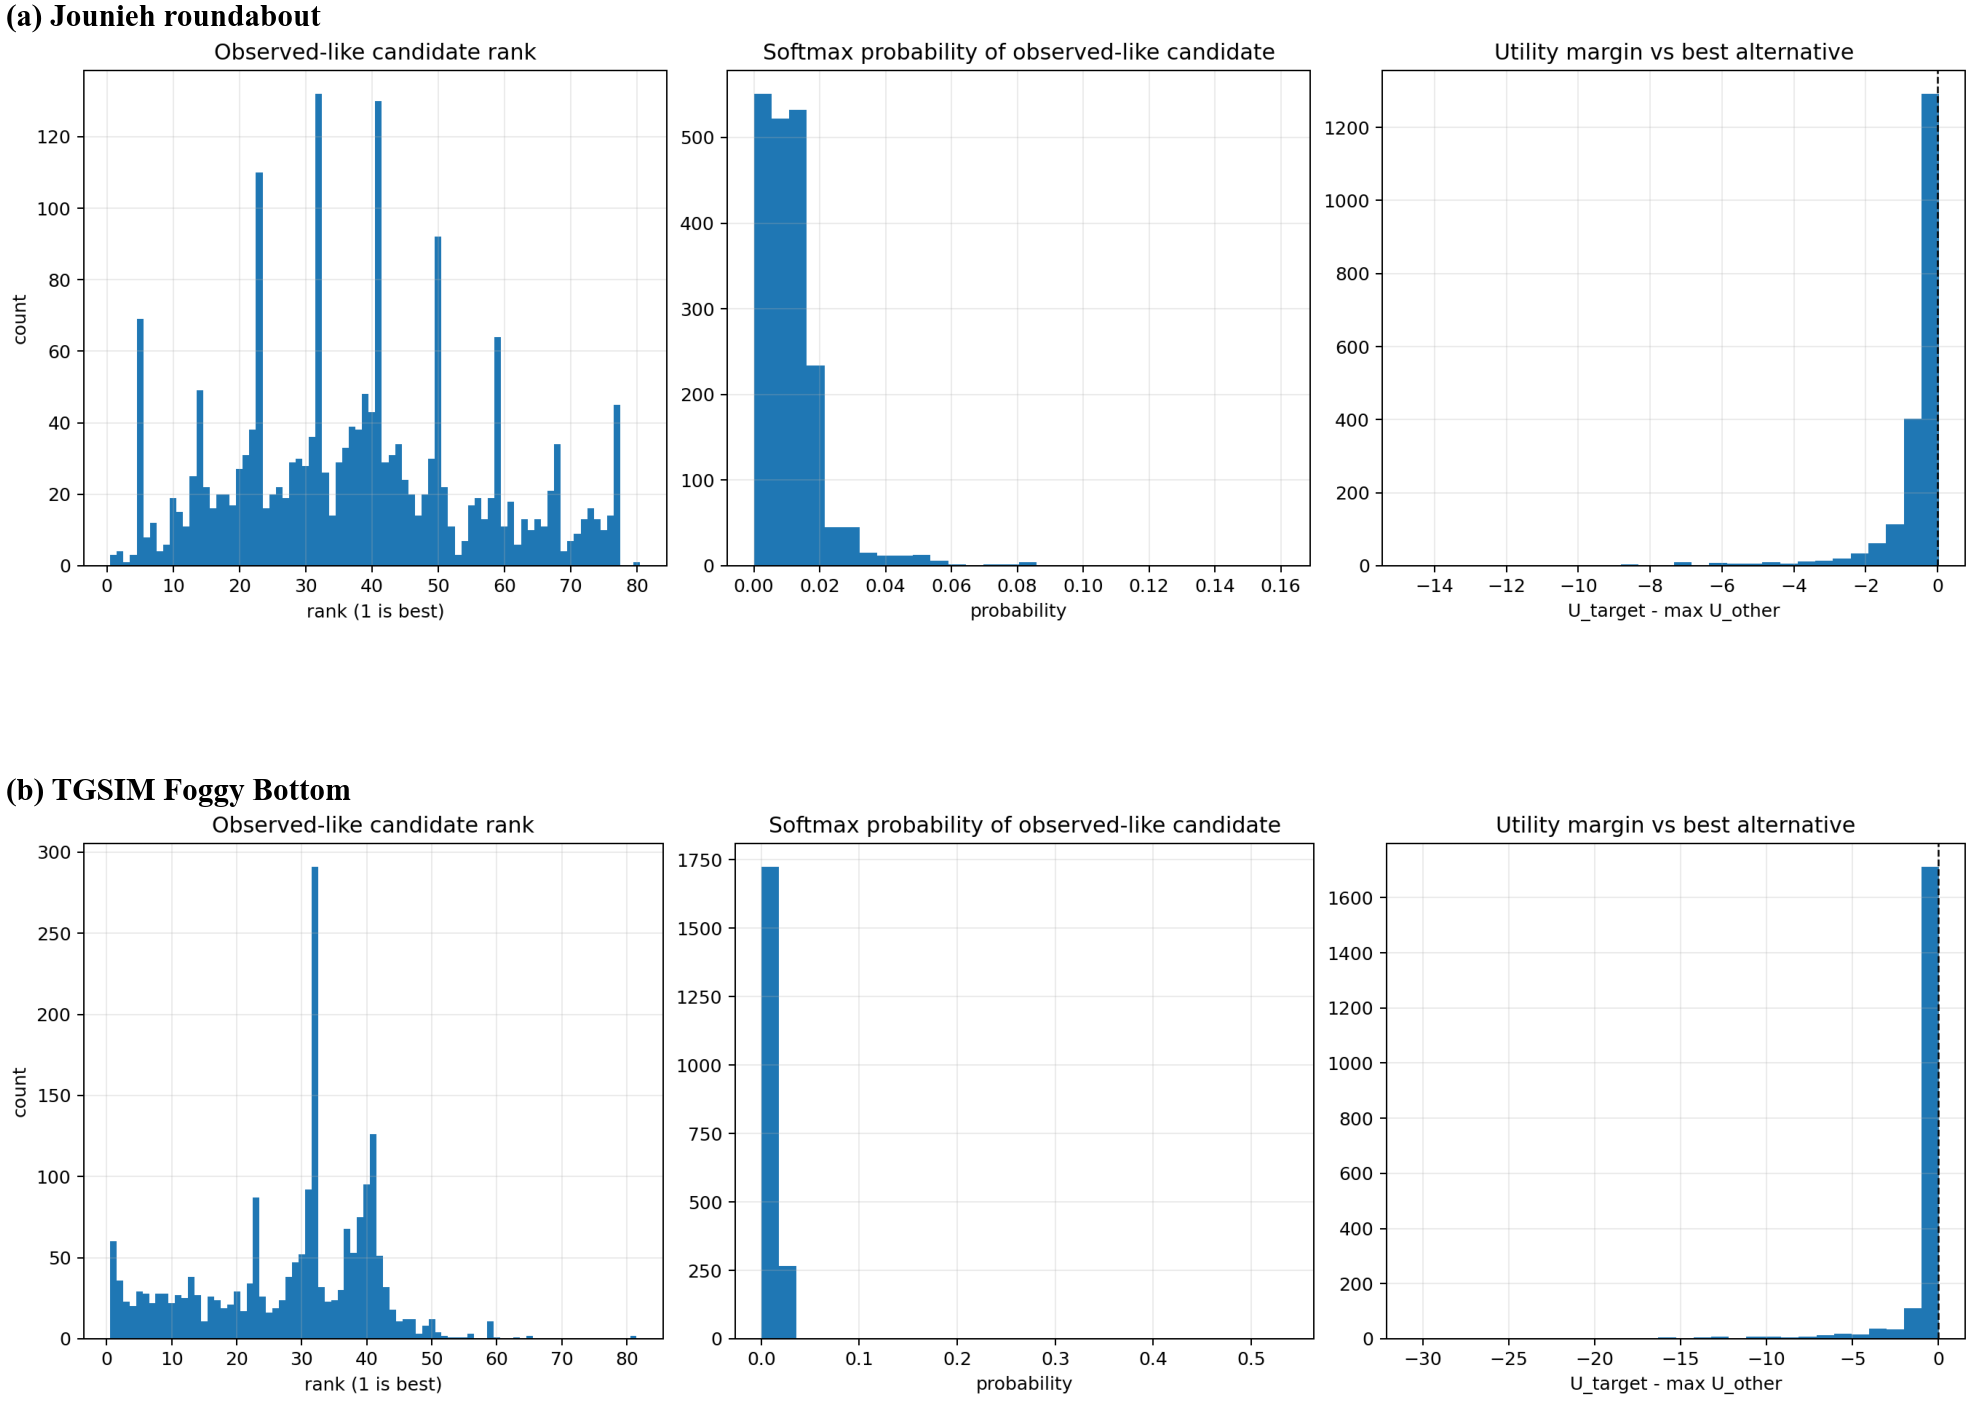
\includegraphics[width=\textwidth]{Appendix/fig_env_calib_fit.png}
\caption{Urban one-step diagnostics under the destination-plus-curb encoding. Left to right in each row: rank of the observed-like candidate, softmax probability of that candidate, and utility margin relative to the best alternative. (a)~Jounieh roundabout. (b)~TGSIM Foggy Bottom. Rank histograms are much flatter than the freeway fit in Fig.~\ref{fig:calibration_fit_quality}, while margins still pile up near zero.}
\label{fig:app_env_fit}
\end{figure*}

\paragraph{What the weights say about geometry.}
Table~\ref{tab:app_env_params} shows that the same parameter box produces quite different operating points. Path weight $w_{\ell}$ is large on the freeway ($77.6$), where the PCA tube is a tight behavioral constraint, and remains large at Foggy Bottom ($68.4$), where the curb is the only thing preventing an intersection-cutting chord to the destination. At the roundabout $w_{\ell}$ collapses to $9.17$: once $U_{\mathrm{dir}}$ and $U_{\mathrm{dist}}$ already follow the circulating on-road path around the islands, an additional curb penalty is only weakly identified and several near-optimal trials trade it off against $S_{\theta}$. Collision weight $w_{c}$ is likewise site-dependent ($300$ / $71$ / $6$), matching the main-text observation that $w_{c}$ is poorly constrained by short windows in which collisions are rare. Foggy Bottom loads directional and speed terms ($S_{\theta}=8.46$, $S_{v}=9.68$) more heavily than the freeway, as would be expected when progress is defined by reaching a destination through a sparse street graph rather than staying in a tube.

\paragraph{Scope.}
These results support transferring the five-term prior across environments \emph{provided} the spatial frame is rewritten for the site (corridor tubes versus destination on a curb polygon). They do not show that one numerical $\theta$ is universal, and they do not replace the freeway residual-MARL study: urban closed-loop errors are larger, identifiability is weaker, and no residual policy was trained at the roundabout or at Foggy Bottom. Per-track overlays remain mixed---many vehicles stay inside the curb and trend toward their destination, while a subset still freeze, cut a corner, or take the wrong exit arm---which is why the population test loss, rather than any single ID, is the quantity reported in Table~\ref{tab:app_env_calib}.

\end{document}